\documentclass[ngerman,a4paper,order=firstname]{../../texmf/tex/latex/mathscript/mathscript}
\usepackage{../../texmf/tex/latex/mathoperators/mathoperators}

\title{\textbf{Lineare Algebra SS2018}}
\author{Dozent: Prof. Dr. Arno Fehm}

\begin{document}
\pagenumbering{roman}
\pagestyle{plain}

\maketitle

\hypertarget{tocpage}{}
\tableofcontents
\bookmark[dest=tocpage,level=1]{Inhaltsverzeichnis}

\pagebreak
\pagenumbering{arabic}
\pagestyle{fancy}

\setcounter{chapter}{4}

\chapter{Endomorphismen}
In diesem Kapitel seien $K$ ein Körper, $n\in\natur$ eine natürliche Zahl, $V$ ein $n$-dimensionaler $K$-Vektorraum und $f\in\End_K(V)$ ein Endomorphismus.

Das Ziel dieses Kapitels ist, die Geometrie von $f$ besser zu verstehen und Basen zu finden, für die $M_B(f)$ eine besonders einfache oder kanonische Form hat.

\section{Eigenwerte}

\begin{remark}
	Wir erinnern uns daran, dass $\End_K(V)=\Hom_K(V,V)$ sowohl einen $K$-Vektorraum als auch einen Ring bildet. Bei der Wahl einer Basis $B$ von $V$ wird $f\in\End_K(V)$ durch die Matrix $M_B(f)=M_B^B(f)$ beschrieben.	
\end{remark}

\begin{example}
	$K=\real, A=\begin{henrysmatrix}1&2\\2&1\end{henrysmatrix}\in\Mat_2(\real),f=f_A\in\End_K(K^2)$ \\
	\begin{align}
		A\cdot \begin{henrysmatrix}1\\1\end{henrysmatrix}=\begin{henrysmatrix}3\\3\end{henrysmatrix},\;A\cdot\begin{henrysmatrix} 1\\-1\end{henrysmatrix}=\begin{henrysmatrix}-1\\1\end{henrysmatrix}\notag
	\end{align}
	$\Rightarrow$ mit $B=\left( \begin{henrysmatrix}1\\1\end{henrysmatrix},\begin{henrysmatrix}1\\-1\end{henrysmatrix}\right)$ ist $M_B(f)=\begin{henrysmatrix}3&0\\0&-1\end{henrysmatrix}$. \\
	Der Endomorphismus $f=f_A$ streckt also entlang der Achse $\real\cdot \begin{henrysmatrix}1\\1\end{henrysmatrix}$ um den Faktor 3 und spiegelt entlang der Achse $\real\cdot \begin{henrysmatrix}1\\-1\end{henrysmatrix}$
	\begin{center}
		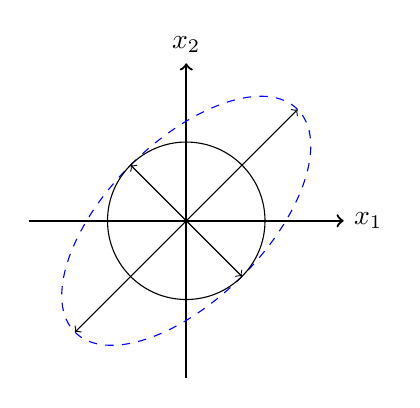
\begin{tikzpicture}
		\draw[->,thick] (-2,0) -- (2,0) node[right] {$x_1$};
		\draw[->,thick] (0,-2) -- (0,2) node[above] {$x_2$};
		\draw[->, thin] (0,0) -- (1.414,1.414);
		\draw[->, thin] (0,0) -- (-1.414,-1.414);
		\draw[->, thin] (0,0) -- (-0.707,0.707);
		\draw[->, thin] (0,0) -- (0.707,-0.707);
		\draw[dashed, rotate=+45, blue] (0,0) ellipse (2cm and 1cm);
		\draw (0,0) circle (1);
		\end{tikzpicture}
	\end{center}
\end{example}

\begin{definition}[Eigenwert, Eigenvektor, Eigenraum]
	Sind $0\neq x\in V$ und $\lambda\in K$ mit $f(x)=\lambda x$ so nennt man $\lambda$ einen \begriff{Eigenwert} von $f$ und $x$ einen \begriff{Eigenvektor} von $f$ zum Eigenwert $\lambda$. Der \begriff{Eigenraum} zu $\lambda\in K$ ist $\Eig (f,\lambda)=\{x\in V\mid f(x)=\lambda x\}$.
\end{definition}

\begin{remark}
	Für jedes $\lambda\in K$ ist $\Eig (f,\lambda)$ ein Untervektorraum von $V$, da
	\begin{align}
		\Eig (f,\lambda) &= \{x\in V\mid f(x)=\lambda x\} \notag \\
		&= \{x\in V\mid f(x)-\lambda\cdot\id_V(x)=0\} \notag \\
		&= \{x\in V\mid (f-\lambda\cdot\id_V)(x)=0\} \notag \\
		&= \Ker (f-\lambda\cdot\id_V) \notag
	\end{align}
	und $f-\lambda\cdot\id_V\in\End_K(V)$.
\end{remark}

\begin{remark}
	Achtung! Der Nullvektor ist nach Definition kein Eigenvektor, aber $\lambda=0$ kann ein Eigenwert sein, nämlich genau dann, wenn $f\notin\Aut_K(V)$, siehe Übung. Die Menge der Eigenvektoren zu $\lambda$ ist also $\Eig (f,\lambda)\backslash\{0\}$ und $\lambda$ ist genau dann ein Eigenwert von $f$, wenn $\Eig (f,\lambda)\neq\{0\}$.
\end{remark}

\begin{example}
	Ist $A=\diag(\lambda_1,...,\lambda_n)$ und $f=f_A\in\End_K(K^n)$, so sind $\lambda_1,...,\lambda_n$ Eigenwerte von $f$ und jedes $e_i$ ist ein Eigenvektor zum Eigenwert $\lambda_i$.
\end{example}

\begin{proposition}
	\proplbl{satz_diagonal_ev}
	Sei $B$ eine Basis von $V$. Genau dann ist $M_B(f)$ eine Diagonalmatrix, wenn $B$ aus Eigenvektoren von $f$ besteht.
\end{proposition}
\begin{proof}
	Ist $B=(x_1,...x_n)$ eine Basis aus Eigenvektoren zu Eigenwerten $\lambda_1,....,\lambda_n$, so ist $M_B(f)= \diag(\lambda_1,...,\lambda_n)$ und umgekehrt.
\end{proof}

\begin{example}
	Sei $K=\real$, $V=\real^2$ und $f_{\alpha}\in\End_K(\real^2)$ die Drehung um den Winkel $\alpha\in [0,2\pi)$ \\
	\[\Rightarrow M_{\mathcal{E}}(f_{\alpha})=\begin{pmatrix}\cos(\alpha)&-\sin(\alpha) \\ \sin(\alpha) & \cos(\alpha)\end{pmatrix}\]
	Für $\alpha=0$ hat $f_{\alpha}=\id_{\real^2}$ nur den Eigenwert 1. \\
	Für $\alpha=\pi$ hat $f_{\alpha}=-\id_{\real^2}$ nur den Eigenwert -1. \\
	Für $\alpha\neq 0,\pi$ hat $f_{\alpha}$ keine Eigenwerte. %TODO figure
\end{example}

\begin{lemma}
	\proplbl{lemma_EW_lin_unabh}
	Sind $\lambda_1,...,\lambda_n$ paarweise verschiedene Eigenwerte von $f$ und ist $x_i$ ein Eigenvektor zu $\lambda_i$ für $i=1,...,m$, so ist $(x_1,...,x_m)$ linear unabhängig.
\end{lemma}
\begin{proof}
	Induktion nach $m$\\
	\emph{$m=1$}: klar, denn $x_1\neq 0$ \\
	\emph{$m-1\to m$}: Sei $\sum_{i=1}^m \mu_i x_i=0$ mit $\mu_1,...,\mu_m\in K$.
	\begin{align}
		0&= (f-\lambda\cdot\id_V)\left( \sum\limits_{i=1}^m \mu_i x_i\right) \notag \\
		&= \sum\limits_{i=1}^m \mu_i(f(x_i)-\lambda_m\cdot x_i) \notag \\
		&= \sum\limits_{i=1}^{m-1} \mu_i(\lambda_i-\lambda_m)\cdot x_i \notag
	\end{align} 
	Nach IB ist $\mu_i(\lambda_i-\lambda_m)=0$ für $i=1,...,m-1$, da $\lambda_i\neq\lambda_m$ für $i\neq m$ also $\mu_i=0$ für $i=1,...,m-1$. Damit ist auch $\mu_m=0$. Folglich ist $(x_1,...,x_m)$ linear unabhängig.
\end{proof}

\begin{proposition}
	\proplbl{satz_eig_direkte_summe}
	Sind $\lambda_1,...,\lambda_m\in K$ paarweise verschieden, so ist 
	\[\sum\limits_{i=1}^m \Eig(f,\lambda_i)=\bigoplus_{i=0}^{m}\Eig(f,\lambda_i).\]
\end{proposition}
\begin{proof}
	Seien $x_i,y_i\in\Eig(f,\lambda_i)$ für $i=1,...,m$. Ist $\sum_{i=1}^m x_i=\sum_{i=1}^m y_i$, so ist $\sum_{i=1}^m \underbrace{x_i-y_i}_{z_i}=0$.\\
	o. E. seien $z_i\neq 0$ für $i=1,...,r$ und $z_i=0$ für $i=r+1,...,m$. Wäre $r>0$, so wären $(z_1,...,z_r)$ linear abhängig, aber $z_i=x_i-y_i\in\Eig(f,\lambda_i)\backslash\{0\}$, im Widerspruch zu \propref{lemma_EW_lin_unabh}. Somit ist $x_i=y_i$ für alle $i$ und folglich ist die Summe $\sum\Eig(f,\lambda_i)$ direkt.
\end{proof}

\begin{definition}[Eigenwerte und Eigenvektoren für Matrizen]
	Sei $A\in\Mat_n(K)$. Man definiert Eigenwerte, Eigenvektoren, etc. von $A$ als Eigenwerte, Eigenvektoren von $f_A\in\End_K(K^n)$.
\end{definition}

\begin{mathematica}[Eigenwerte und Eigenvektoren]
	Um die Eigenwerte und Eigenvektoren einer Matrix $A$ zu berechnen, gibt es in Mathematica bzw. WolframAlpha verschiedene Möglichkeiten:
	\begin{itemize}
		\item \texttt{Eigenvalues[A]}: liefert eine Liste der Eigenwerte
		\item \texttt{Eigenvectors[A]}: liefert eine Liste der Eigenvektoren
		\item \texttt{Eigensystem[A]}: liefert zu jeden Eigenwert den Eigenvektor
	\end{itemize}
\end{mathematica}

\begin{proposition}
	Sei $B$ eine Basis von $V$ und $\lambda\in K$. Genau dann ist $\lambda$ ein Eigenvektor von $f$, wenn $\lambda$ ein Eigenwert von $A=M_B(f)$ ist. Insbesondere haben ähnliche Matrizen die selben Eigenwerte.
\end{proposition}
\begin{proof}
	Dies folgt aus dem kommutativen Diagramm
	\begin{center}\begin{tikzpicture}
		\matrix (m) [matrix of math nodes,row sep=3em,column sep=4em,minimum width=2em]
		{K^n & K^n \\ V & V \\};
		\path[-stealth]
		(m-1-1) edge node [left] {$\Phi_B$} (m-2-1)
		edge node [above] {$f_A$} (m-1-2)
		(m-2-1) edge node [below] {$f$} (m-2-2)
		(m-1-2) edge node [right] {$\Phi_B$} (m-2-2);
		\end{tikzpicture}\end{center}
	denn $f_A(x)=\lambda x\iff (\Phi_B\circ f_A)(x)=\Phi_B(\lambda x)\iff f(\Phi_B(x))=\lambda\Phi_B(x)$. \\
	Ähnliche Matrizen beschreiben den selben Endomorphismus bezüglich verschiedener Basen, vgl. \propref{4_4_1}
\end{proof}
\section{Das charakteristische Polynom}

\begin{proposition}
	\proplbl{satz_det_null}
	Sei $\lambda\in K$. Genau dann ist $\lambda$ ein EW von $f$, wenn $\det(\lambda\cdot\id_V-f)=0$.
\end{proposition}
\begin{proof}
	Da $\Eig(f,\lambda)=\Ker(\lambda\cdot\id_V-f)$ ist $\lambda$ genau dann ein EW von $f$, wenn $\dim_K(\Ker(\lambda\cdot\id_V-f))>0$, also wenn $\lambda\cdot\id_V-f\notin\Aut_K(V)$. Nach IV.4.6 bedeutet dies, dass $\det(\lambda\cdot\id_V-f)=0$ %TODO: Verlinkung setzen
\end{proof}

\begin{definition}[charakteristisches Polynom]
	Das \begriff{charakteristische Polynom} einer Matrix $A\in\Mat_n(K)$ ist die Determinante der Matrix $t\cdot \mathbbm{1}_n-A\in\Mat_n(K[t])$. 
	\begin{align}
		\chi_A(t)&=\det(t\cdot \mathbbm{1}_n-A)\in K[t] \notag
	\end{align}
	Das charakteristische Polynom eines Endomorphismus $f\in\End_K(V)$ ist $\chi_f(t)=\chi_{M_B(f)}(t)$, wobei $B$ eine Basis von $V$ ist.
\end{definition}

\begin{proposition}
	\proplbl{satz_2_3}
	Sind $A,B\in\Mat_n(K)$ mit $A\sim B$, so ist $\chi_A=\chi_B$. Insbesondere ist $\chi_f$ wohldefiniert.
\end{proposition}
\begin{proof}
	Ist $B=SAS^{-1}$ mit $S\in\GL_n(K)$, so ist $t\cdot \mathbbm{1}_n-B = S(t\cdot \mathbbm{1}_n-A)S^{-1}$, also $t\cdot \mathbbm{1}_n-B\sim t\cdot \mathbbm{1}_n-A$ und ähnliche Matrizen haben die selben Determinante (IV.4.4). \\
	Sind $B,B'$ Basen von $V$, so sind $M_B(f)\sim M_{B'}(f)$, also $\chi_{M_B(f)}=\chi_{M_{B'}(f)}$ %TODO: Verlinkung setzen
\end{proof}

\begin{lemma}
	\proplbl{lemma_chi_det}
	Für $\lambda\in K$ ist $\chi_f(\lambda)=\det(\lambda\cdot\id_V-f)$.
\end{lemma}
\begin{proof}
	Sei $B$ eine Basis von $V$ und $A=M_B(f)=(a_{ij})_{i,j}$. Dann ist $M_B(\lambda\cdot\id_V-f)= \lambda\cdot \mathbbm{1}_n-A$. Aus IV.2.8 und I.6.8 folgt $\det(t\cdot \mathbbm{1}_n-A)(\lambda)=\det(\lambda\cdot \mathbbm{1}_n-A)$. Folglich ist 
	\begin{align}
		\chi_f(\lambda)&=\chi_A(\lambda)\notag \\
		&=\det(t\cdot \mathbbm{1}_n-A)(\lambda)\notag \\
		&=\det(\lambda\cdot \mathbbm{1}_n-A)\notag \\
		&= \det(\lambda\cdot\id_V-f) \notag
	\end{align}
\end{proof}

\begin{proposition}
	\proplbl{satz_chi_polynom}
	Sei $\dim_K(V)=n$ und $f\in\End_K(V)$. Dann ist $\chi_f(t)=\sum_{i=0}^n \alpha_i t^i$ ein Polynom vom Grad $n$ mit 
	\begin{align}
		\alpha_n&=1\notag \\
		\alpha_{n-1}&=-\tr(f) \notag \\
		\alpha_0 &= (-1)^n\cdot\det(f) \notag
	\end{align}
	Die Nullstellen von $\chi_f$ sind genau die EW von $f$.
\end{proposition}
\begin{proof}
	Sei $B$ eine Basis von $V$ und $A=M_B(f)=(a_{ij})_{i,j}$. Wir erinnern uns daran, dass $\tr(f)=\tr(A=\sum_{i=1}^n a_{ii}$. Es ist $\chi_f(t)=\det(t-\cdot 1_n-A)=\sum_{\sigma\in S_n}\sgn(\sigma)\prod_{i=1}^n (t\delta_{i,\sigma(i)}-a_{i,\sigma(i)})$. \\
	Der Summand für \emph{$\sigma=\id$} ist $\prod_{i=1}^n (t-a_{ii})=t^n+\sum_{i=1}^n (-a_{ii})t^{n-1}+...+\prod_{i=1}^n(-a_{ii})$ \\
	Für \emph{$\sigma\neq\id$} ist $\sigma(i)\neq i$ für mindestens zwei $i$, der entsprechende Summand hat also Grad höchstens $n-2$. Somit haben $\alpha_n$ und $\alpha_{n-1}$ die oben behauptete Form, und $\alpha_0=\chi_A(0)=\det(-A)=(-1)^n\cdot\det(f)$. \\
	Die Aussage über die Nullstellen von $\chi_f$ folgt aus \propref{satz_det_null} und \propref{lemma_chi_det}.
\end{proof}

\begin{conclusion}
	Ist $\dim_K(V)=n$, so hat $f$ höchstens $n$ Eigenwerte.
\end{conclusion}
\begin{proof}
	\propref{satz_chi_polynom} und I.6.10 %TODO: Verlinkung
\end{proof}

\begin{definition}[normiertes Polynom]
	Ein Polynom $0\neq P\in K[t]$ mit Leitkoeffizient 1 heißt \begriff{normiert}.
\end{definition}

\begin{example}
	\proplbl{beispiel_2_8}
	\begin{enumerate}
		\item Ist $A=(a_{ij})_{i,j}$ eine obere Dreiecksmatrix, so ist $\chi_A(t)=\prod_{i=1}^n (t-a_{ii})$, vgl. IV.2.9.c \\ %TODO: Verlinkung
		Insbesondere ist $\chi_{1_n}(t)=(t-1)^n$, $\chi_0(t)=t^n$
		\item Für eine Blockmatrix $A=\begin{pmatrix}A_1&B \\ 0&A_2\end{pmatrix}$ mit quadratischen Matrizen $A_1,A_2$ ist $\chi_A=\chi_{A_1}\cdot \chi_{A_2}$ vgl. IV.2.9.e %TODO: Verlinkung
		\item Für
		\begin{align}
			\begin{pmatrix}
			0&...&...&...&0&-c_0  \\ 
			1& \ddots&\;&\;&\vdots&\vdots  \\ 
			0&\ddots&\ddots&\;&\vdots&\vdots  \\ 
			\vdots&\ddots&\ddots&\ddots&\vdots&\vdots  \\ 
			0&...&0&1&0&-c_{n-1} 
			\end{pmatrix} \quad c_0,...,c_{n-1}\in K \notag
		\end{align}
		ist $\chi_A(t)=t^n+\sum_{i=0}^{n-1} c_i t^i$ \\
		Man nennt diese Matrix die Begleitmatrix zum normierten Polynom $P=t^n+\sum_{i=0}^{n-1} c_i t^i$ und schreibt $M_P:=A$
	\end{enumerate}
\end{example}
\section{Diagonalisierbarkeit}

\begin{definition}[diagonalisierbar]
	Man nennt $f$ \begriff{diagonalisierbar}, wenn $V$ eine Basis $B$ besitzt, für die $M_B(f)$ eine Diagonalmatrix ist.
\end{definition}

\begin{lemma}
	\proplbl{lemma_diag_summe_eig}
	Genau dann ist $f$ diagonalisierbar, wenn
	\begin{align}
		V=\sum\limits_{\lambda\in K} \Eig(f,\lambda) \notag
	\end{align}.
\end{lemma}
\begin{proof}
	$(\Rightarrow)$: Ist $B$ eine Basis aus EV von $f$ (vgl. \propref{satz_diagonal_ev}), so ist $B\le \bigcup\limits_{\lambda\in K}\Eig(f,\lambda)$, also $V=\Span_K(\bigcup\limits_{\lambda\in K}\Eig(f, \lambda))=\sum\limits_{\lambda\in K}\Eig(f,\lambda)$. \\
	$(\Leftarrow)$: Ist $V=\sum\limits_{\lambda\in K}\Eig(f,\lambda)$, so gibt es $\lambda_1,...,\lambda_n \in K$ mit $V=\sum\limits_{i=1}^r \Eig(f,\lambda_i)$. Wir wählen Basen $B_i$ von $\Eig(f,\lambda_i)$. Dann ist $\bigcup\limits_{i=1}^r B_i$ ein endliches Erzeugendensystem von $V$, enthält also eine Basis von $V$ (II.3.6). Diese besteht aus EV von $f$. %TODO: Verlinkung
\end{proof}

\begin{proposition}
	Ist $\dim_K(V)=n$, so hat $f$ höchstens $n$ Eigenwerte. Hat $f$ genau $n$ Eigenwerte, so ist $f$ diagonalisierbar.
\end{proposition}
\begin{proof}
	Ist $\lambda$ ein EW von $f$, so ist $\dim_K(\Eig(f,\lambda))\ge 1$. Sind also $\lambda_1,...,\lambda_n$ paarweise verschiedene EW von $f$, so ist
	\begin{align}
		n=\dim_K(V)&\ge \dim_K\left( \sum\limits_{i=1}^m \Eig(f,\lambda_i)\right) \notag \\
		&\overset{\text{\propref{satz_eig_direkte_summe}}}{=} \dim_K\left( \bigoplus_{i=0}^{m} \Eig(f,\lambda_i)\right) \notag \\
		&= \sum\limits_{i=1}^m \dim_K(\Eig(f,\lambda_i)) \notag \\
		&\ge m \notag
	\end{align}
	Ist zudem $m=n$, so muss 
	\begin{align}
		\dim_K(V) &= \dim_K(\sum\limits_{i=1}^m \Eig(f,\lambda_i))\text{ sein, also }\notag \\
		V&= \sum\limits_{i=1}^m \Eig(f,\lambda_i) \notag
	\end{align}
	Nach \propref{lemma_diag_summe_eig} ist $f$ genau dann diagonalisierbar.
\end{proof}

\begin{definition}[$a$ teilt $b$]
	Sei $R$ ein kommutativer Ring mit seien $a,b\in R$. Man sagt, $a$ \begriff{teilt} $b$ (in Zeichen $a\vert b$), wenn es $x\in R$ mit $b=ax$ gibt.
\end{definition}

\begin{definition}[Vielfachheit]
	Für $0\neq P\in K[t]$ und $\lambda\in K$ nennt man $\mu(P,\lambda)=\max\{r\in \natur_{>0}\mid (t-r)^r\vert P\}$ die \begriff{Vielfachheit} der Nullstelle $\lambda$ von $P$.
\end{definition}

\begin{lemma}
	\proplbl{lemma_3_6}
	Genau dann ist $\mu(P,\lambda)\ge 1$, wenn $\lambda$ eine Nullstelle von $P$ ist.
\end{lemma}
\begin{proof}
	$(\Rightarrow)$: $t-\lambda\vert P\Rightarrow P(t)=(t-\lambda)\cdot Q(t)$ mit $Q(t)\in K[t]\Rightarrow P(\lambda)=0\cdot Q(\lambda)=0$. \\
	$(\Leftarrow)$: $P(\lambda)=0\overset{I.6.9}{=}t-\lambda\vert P(t)\Rightarrow \mu(P,\lambda)\ge 1$.
	%TODO: Verlinkung
\end{proof}

\begin{lemma}
	\proplbl{lemma_3_7}
	Ist $P(t)=(t-\lambda)^r\cdot Q(t)$ mit $Q(t)\in K[t]$ und $Q(\lambda)\neq 0$, so ist $\mu(P,\lambda)=r$
\end{lemma}
\begin{proof}
	Offensichtlich ist $\mu(P,\lambda)\ge r$. Wäre $\mu(P,\lambda)\ge r+l$, so $(t-\lambda)^{r+l}\vert P(t)$ also $(t-\lambda)^r\cdot Q(t)=(t-\lambda)^{r^+l}\cdot R(t)$ mit $R(t)\in K[t]$, folglich $t-\lambda\vert Q(t)$, insbesondere $Q(\lambda)=0$. \\
	(Denn wir dürfen kürzen: $R$ ist nullteilerfrei, genau so wie $K[t]$). \\
	$(t-\lambda)^r(Q(t)-(t-\lambda)R(t))=0\Rightarrow Q(t)=(t-\lambda)R(t)$.
\end{proof}

\begin{lemma}
	\proplbl{lemma_3_8}
	Sind $P,Q,R\in K[t]$ mit $PQ=PR$, und ist $P\neq 0$, so ist $Q=R$.
\end{lemma}
\begin{proof}
	$PQ=PR\Rightarrow P(Q-R)=0\overset{K[t]\text{ nullteilerfrei}}{\Rightarrow} Q-R=0$, d.h. $Q=R$.
\end{proof}

\begin{lemma}
	\proplbl{lemma_3_9}
	Es ist $\sum\limits_{\lambda\in K} \mu(P,\lambda)\le \deg(P)$, mit Gleichheit genau dann, wenn $P$ in Linearfaktoren zerfällt.
\end{lemma}
\begin{proof}
	Schreibe $P(t)=\prod\limits_{\lambda\in K}(t-\lambda)^{r_\lambda}\cdot Q(t)$, wobei $Q(t)\in K[t]$ keine Nullstellen mehr besitzt. Nach \propref{lemma_3_7} ist $\mu(P,\lambda)=r_\lambda$ für alle $\lambda$ und somit $\deg(P)=\sum\limits_{\lambda\in K} r_\lambda+\deg(Q)\ge \sum\limits_{\lambda\in K} \mu(P,\lambda)$ mit Gleichheit genau dann,wenn $\deg(Q)=0$, also $Q=c\in K$, d.h. genau dann, wenn $P(t)=c\cdot \prod\limits_{\lambda\in K} (t-\lambda)^{r_\lambda}$.
\end{proof}

\begin{lemma}
	\proplbl{lemma_3_10}
	Für $\lambda\in K$ ist
	\begin{align}
		\dim_K(\Eig(f,\lambda))\ge \mu(x_f,\lambda)\notag
	\end{align}
\end{lemma}
\begin{proof}
	Ergänze eine Basis $B$ von $\Eig(f,\lambda)$ zu einer Basis $B$ von $V$. Dann ist 
	\begin{align}
		A=M_B(f)=\begin{pmatrix}\lambda\mathbbm{1}_s&*\\0&A'\end{pmatrix}\notag
	\end{align}
	mit einer Matrix $A'\in \Mat_{n-s}(K)$, also $\chi_f(t)=\chi_A(t)\overset{\text{\propref{beispiel_2_8}}}{=}\chi_{\lambda\mathbbm{1}}\cdot\chi_{A'}(t)=(t- \lambda)^s\cdot \chi_{A'}(t)$ und somit $\dim_K(\Eig(f,\lambda))=s\le \mu(x_f,\lambda)$.
\end{proof}

\begin{proposition}
	Genau dann ist $f$ diagonalisierbar, wenn $\chi_f$ in Linearfaktoren zerfällt und $\dim_K(\Eig(f,\lambda))=\mu(x_f,\lambda)$ für alle $\lambda\in K$.
\end{proposition}
\begin{proof}
	Es gilt
	\begin{align}
		\dim_K(\sum\limits_{\lambda\in K}\Eig(f,\lambda))&\overset{\text{\propref{satz_eig_direkte_summe}}}{=} \dim_K(\bigoplus\limits_{\lambda\in K}\Eig(f,\lambda)) \notag \\
		&\overset{\text{II.4.12}}{=}\sum\limits_{\lambda\in K}\dim_K(\Eig(f,\lambda)) \notag \\
		&\overset{\text{\propref{lemma_3_10}}}{\le}\sum\limits_{\lambda\in K}\mu(\chi_f,\lambda) \\
		&\le \deg(\chi_f) \\
		&= n \notag
	\end{align}
	Nach \propref{lemma_diag_summe_eig} ist $f$ genau dann diagonalisierbar, wenn $\dim_K(\sum\limits_{\lambda\in K}\Eig(f,\lambda))=n$, also wenn bei (1) und (2) Gleichheit herrscht. Gleichheit bei (1) bedeutet $\dim_K(\Eig(f,\lambda))=\mu(\chi_f,\lambda)$ für alle $\lambda\in K$, und Gleichheit bei (2) bedeutet nach \propref{lemma_3_9}, dass $\chi_f$ in Linearfaktoren zerfällt. %TODO: Verlinkung
\end{proof}

\begin{definition}[algebraische und geometrische Vielfachheit]
	Man nennt $\mu_a(f,\lambda)=\mu(\chi_f,\lambda)$ die \begriff[Vielfachheit!]{algebraische Vielfachheit} und $\mu_g(f,\lambda)=\dim_K(\Eig(f,\lambda))$ die  \begriff[Vielfachheit!]{geometrische Vielfachheit} des Eigenwertes $\lambda$ von $f$.
\end{definition}

\begin{remark}
	Wieder nennt man $A\in\Mat_n(K)$ diagonalisierbar, wenn $f_A\in\End_K(K^n)$ diagonalisierbar ist, also wenn $A\sim D$ für eine Diagonalmatrix $D$.
\end{remark}
\section{Trigonalisierbarkeit}

\begin{definition}
	Man nennt $f$ \begriff{trigonalisierbar}, wenn $V$ eine Basis $B$ besitzt, für die $M_B(f)$ eine obere Dreiecksmatrix ist.
\end{definition}

\begin{example}
	Ist $f$ diagonalisierbar, so ist $f$ auch trigonalisierbar.
\end{example}

\begin{lemma}
	\proplbl{lemma_4_3}
	Ist $f$ trigonalisierbar, so zerfällt $\chi_f$ in Linearfaktoren.
\end{lemma}
\begin{proof}
	Klar aus \propref{beispiel_2_8} und \propref{satz_2_3}.
\end{proof}

\begin{definition}[invariant]
	Ein Untervektorraum $W\le V$ ist $f$-\begriff{invariant}, wenn $f(W)\le W$.
\end{definition}

\begin{remark}
	Ist $W$ ein $f$-invarianter UVR von $V$, so ist $f\vert_W\in \End_K(W)$.
\end{remark}

\begin{example}
	\proplbl{beispiel_4_6}
	\begin{enumerate}
		\item $V$ hat stets die $f$-invarianten UVR $W=\{0\}$ und $W=V$.
		\item Jeder UVR $W\le \Eig(f,\lambda)$ ist $f$-invariant.
		\item Ist $B=(x_1,...,x_n)$ eine Basis von $V$, für die $M_B(f)$ eine obere Dreiecksmatrix ist, so sind alle UVR $W_i=\Span_K(x_1,...,x_i)$ $f$-invariant.
		\item Sei $V=W\oplus U$, $B_1=(x_1,...,x_r)$ Basis von $W$, $B_2(x_{r+1},...,x_n)$ Basis von $U$ und $B=(x_1,...,x_n)$. Ist $W$ $f$-invariant, so ist 
		\begin{align}
			M_B(f)=\begin{pmatrix}M_{B_1}(f\vert_W)&*\\0&*\end{pmatrix}\notag
		\end{align}
		Sind $W$ und $U$ $f$-invariant, so ist 
		\begin{align}
			M_B(f)=\begin{pmatrix}M_{B_1}(f\vert_W)&0\\0&M_{B_2}(f\vert_U)\end{pmatrix}\notag
		\end{align}
	\end{enumerate}
\end{example}

\begin{lemma}
	Ist $W\subset V$ ein $f$-invarianter UVR, so gilt $\chi_{f\vert_W}\vert \chi_f$. Hat $W$ ein lineares Komplement $U$, dass auch $f$-invariant ist, so $\chi_f=\chi_{f\vert_W}\cdot \chi_{f\vert_U}$.
\end{lemma}
\begin{proof}
	Ergänze eine Basis $B_0=(x_1,...,x_r)$ von $W$ zu einer Basis $B=(x_1,...,x_n)$ von $V$. Sei $A=M_B(f)$, $A_0=M_{B_0}(f\vert_W)$. Dann ist 
	\begin{align}
		A=\begin{pmatrix}A_0&*\\0&C\end{pmatrix}\quad C\in\Mat_{n-r}(K)\notag
	\end{align}
	folglich $\chi_f=\chi_A=\chi_{A_0}\cdot \chi_C$, insbesondere $\chi_{f\vert_W}\vert\chi_f$.\\
	Ist auch $U=\Span_K(x_{r+1},...,x_n)$ $f$-invariant, so ist 
	\begin{align}
		A=\begin{pmatrix}A_0&0\\0&C\end{pmatrix}\notag
	\end{align}
	und folglich $\chi_f=\chi_A=\chi_{A_0}\cdot\chi_C=\chi_{f\vert_W}\cdot\chi_{f\vert_U}$.
\end{proof}

\begin{theorem}
	Genau dann ist $f$ trigonalisierbar, wenn $\chi_f$ in Linearfaktoren zerfällt.
\end{theorem}
\begin{proof}
	$(\Rightarrow)$: \propref{lemma_4_3}\\
	$(\Leftarrow)$: Induktion nach $n=\dim_K(V)$. \\
	\emph{$n=1$}: trivial \\
	\emph{$n-1\to n$}: Nach Annahme ist $\chi_f(t)=\prod\limits_{i=1}^n (t-\lambda_i)$ mit $\lambda_1,...,\lambda_n\in K$. Sei $x_1$ ein EV zum EW $\lambda_1$. Dann ist $V_1=K\cdot x_1$ ein $f$-invarianter UVR. Ergänze $B_1=(x_1)$ zu einer Basis $B=(x_1,...,x_n)$ von $V$ und setze $B_2=(x_2,...,x_n)$, $V_2=\Span_K(B_2)$.
	\begin{align}
		\Rightarrow M_B(f)&=\begin{pmatrix}\lambda_1&*\\0&A_2\end{pmatrix}\quad A_2\in\Mat_{n-1}(K)\notag\\
		\chi_f(t)&=\chi_{\lambda_1\mathbbm{1}_1}\cdot \chi_{A_2}=(t-\lambda_1)\cdot\chi_{A_2}(t)\notag \\
		\overset{\text{\propref{lemma_3_7}}}{\Rightarrow} \chi_{A_2}(t)&=\prod\limits_{i=2}^n(t-\lambda_i)\notag
	\end{align}
	Seien $\pi_1,\pi_2\in\End_K(V)$ gegeben durch $M_B(\pi_1)=\diag(1,0,...,0)$ und $M_B(\pi_2)=\diag(0,1,...,1)$. Dann ist $\pi_1+\pi_2=\id_V$ und $f_i=\pi_1\circ f$ ist $f=\id_V\circ f=f_1+f_2$ und $f_2\vert_{V_2}\in\End_K(V_2)$. Nach Induktionshypothese ist $f_2\vert_{V_2}$ trigonalisierbar, da $M_B(f_2\vert_{V_2})=A_2$, also $\chi_{f_2\vert_{V_2}}=\chi_{A_2}$. Dies bedeutet, es gibt also eine Basis $B'_2=(x'_2,...,x'_n)$ von $V_2$, für die $M_{B'_2}(f_2\vert_{V_2})$ eine obere Dreiecksmatrix ist. Somit ist für $B'=(x_1,x'_2,...,x'_n)$ auch 
	\begin{align}
		M_{B'}(f)&=M_{B'}(f_1)+M_{B'}(f_2)\notag \\
		&= \begin{pmatrix}\lambda_1&*\\0&0\end{pmatrix} + \begin{pmatrix}0&0\\0&M_{B'_2}(f_2\vert_{V_2})\end{pmatrix}\notag
	\end{align}
	eine obere Dreiecksmatrix.
\end{proof}

\begin{conclusion}
	Ist $K$ algebraisch abgeschlossen, so ist jedes $f\in\End_K(V)$ trigonalisierbar.
\end{conclusion}
\begin{proof}
	Ist $K$ algebraisch abgeschlossen, so zerfällt nach I.6.14 jedes Polynom über $K$ in Linearfaktoren, insbesondere also $\chi_f$. %TODO:Verlinkung
\end{proof}

\begin{conclusion}
	Ist $V$ ein endlichdimensionaler $\comp$-VR, so ist jedes $f\in\End_\comp(V)$ trigonalisierbar.
\end{conclusion}
\begin{proof}
	Nach dem Fundamentalsatz der Algebra I.6.16 ist $\comp$ algebraisch abgeschlossen. %TODO:Verlinkung
\end{proof}
\section{Das Minimalpolynom}

\begin{definition}
	Für ein Polynom $P(t)=\sum_{i=0}^n c_it^i\in K[t]$ definieren wir $P(f)=\sum_{i=0}^m c_if^i\in\End_K(V)$, wobei $f^0=\id_V$, $f^1=f$, $f^2=f\circ f$, ...
	
	Analog definiert man $P(A)$ für $A\in\Mat_n(K)$.
\end{definition}

\begin{remark}
	Die Abbildung $\quad\begin{cases}K[t]\to \End_K(V)\\ P\mapsto P(f)\end{cases}$ ist ein Homomorphismus von $K$-VR und Ringen. Sein Kern ist das Ideal 
	\begin{align}
		\mathcal{I}_f:=\{P\in K[t]\mid P(f)=0\}\notag
	\end{align}
	und sein Bild ist der kommutative Unterring 
	\begin{align}
		K[f]:&=\{P(f)\mid P\in K[t]\}\notag \\
		&= \Span_K(f^0,f^1,f^2,...)\notag
	\end{align}
	des (im Allgemeinen nicht kommutativen) Rings $\End_K(V)$.
	
	Analog definiert man $\mathcal{I}_A$ und $K[A]\le \Mat_n(K)$.
\end{remark}

\begin{lemma}
	\proplbl{lemma_5_3}
	$\mathcal{I}_f\neq\{0\}$
\end{lemma}
\begin{proof}
	Wäre $\mathcal{I}_f=\{0\}$, so wäre $K[t]\to \End_K(V)$ injektiv, aber $\dim_K(K[t])= \infty>n^2=\dim_K(\End_K(V))$, ein Widerspruch.
\end{proof}

\begin{proposition}
	\proplbl{satz_5_4}
	Es gibt ein eindeutig bestimmtes normiertes Polynom $0\neq P\in K[t]$ kleinsten Grades mit $P(f)=0$. Dieses teilt jedes $Q\in K[t]$ mit $Q(f)=0$.
\end{proposition}
\begin{proof}
	Nach \propref{lemma_5_3} gibt es $0\neq P\in K[t]$ mit $P(f)=0$ von minimalem Grad $d$. Indem wir durch den Leitkoeffizienten von $P$ teilen, können wir annehmen, dass $P$ normiert ist. \\
	Sei $Q\in\mathcal{I}_f$. Polynomdivision liefert $R,H\in K[t]$ mit $Q=P\cdot H+R$ und $\deg(R)<\deg(P)=d$. Es folgt $R(f)=\underbrace{Q(f)}_{=0}-\underbrace{P(f)}_{=0}\cdot H(f)=0$. Aus der Minimalität von $d$ folgt $R=0$ und somit $P\mid Q$. \\
	Ist $Q$ zudem normiert vom Grad $d$, so ist $H=1$, also $Q=P$, was die Eindeutigkeit zeigt.
\end{proof}

\begin{definition}[Minimalpolynom]
	Das eindeutig bestimmte normierte Polynom $0\neq P\in K[t]$ kleinsten Grades mit $P(f)=0$ nennt man das \begriff{Minimalpolynom} $P_f$ von $f$.
	
	Analog definiert man das Minimalpolynom $P_A\in K[t]$ einer Matrix $A\in\Mat_n(K)$.
\end{definition}

\begin{mathematica}[Minimalpolynom]
	Die Funktion für das Minimalpolynom $p$ mit der Variable $t$ in Mathematica bzw. WolframAlpha lautet:
	\begin{align}
		\texttt{MinimalPolynomial[p,x]}\notag
	\end{align}
\end{mathematica}

\begin{example}
	\begin{enumerate}
		\item $A=\mathbbm{1}_n$, $\chi_A(t)=(t-1)^n$, $P_A(t)=t-1$
		\item $A=0$, $\chi_A(t)=t^n$, $P_A(t)=t$
		\item Ist $A=\diag(a_1,...,a_n)$ mit paarweise verschiedenen Eigenwerten $\lambda_1,...,\lambda_r$, so ist $\chi_A(t)=\prod_{i=1}^n (t-a_i)=\prod_{i=1}^n (t-\lambda_i)^{\mu_a(f_A,\lambda_i)}$, $P_A(t)=\prod_{i=1}^r (t-\lambda_i)$ und es folgt $\deg(P_A)\ge \vert \{a_1,...,a_n\}\vert=r$.
	\end{enumerate}
\end{example}

\begin{definition}[$f$-zyklisch]
	Ein $f$-invarianter UVR $W\le V$ heißt $f$-\begriff{zyklisch}, wenn es ein $x\in W$ mit $W=\Span_K(x,f(x),f^2(x),...)$ gibt.
\end{definition}

\begin{lemma}
	\proplbl{lemma_5_8}
	Sei $x\in V$ und $x_i=f(x)$. Es gibt ein kleinstes $k$ mit $x_k\in\Span_K(x_0,x_1,...,x_{k-1})$, und $W=\Span_K(x_0,...,x_{k-1})$ ein $f$-zyklischer UVR von $V$ mit Basis $B=(x_0,...,x_{k-1})$ und $M_B(f\vert_W)=M_{\chi_{f\vert_W}}$.
\end{lemma}
\begin{proof}
	Da $\dim_K(V)=n$ ist $(x_0,...,x_n)$ linear abhängig, es gibt also ein kleinstes $k$ mit $(x_0,...,x_{k-1})$ linear unabhängig, aber $(x_0,...,x_k)$ linear abhängig, folglich $x_k\in\Span_K(x_0,...,x_{k-1})$. Mit $x_k=f(x_{k-1})=\sum_{i=0}^{k-1}-c_ix_i$ ist dann 
	Da $\dim_K(V)=n$ ist $(x_0,...,x_n)$ linear abhängig, es gibt also ein kleinstes $k$ mit $(x_0,...,x_{k-1})$ linear unabhängig, aber $(x_0,...,x_k)$ linear abhängig, folglich $x_k\in\Span_K(x_0,...,x_{k-1})$. Mit $x_k=f(x_{k-1})=\sum_{i=0}^{k-1}-c_ix_i$ ist dann 
	\begin{align}
		M_B(f\vert_W)=\begin{pmatrix}0&...&...&...&0&-c_0\\
		1&\ddots&\;&\;&\vdots&\vdots\\
		0&\ddots&\ddots&\;&\vdots&\vdots\\
		\vdots&\ddots&\ddots&\ddots&\vdots&\vdots\\
		0&...&0&1&0&-c_{k-1}\end{pmatrix}\notag
	\end{align}
	somit $\chi_{f\vert_W}=t^k+\sum_{i=0}^{k-1}c_it^i$, also $M_B(f\vert_W)=M_{\chi_{f\vert_W}}$.
\end{proof}

\begin{theorem}[Satz von \person{Cayley-Hamiltion}]
	\proplbl{theorem_5_9}
	Für $f\in\End_K(V)$ ist $\chi_f(f)=0$.
\end{theorem}
\begin{proof}
	Sei $x\in V$. Definiere $x_i=f^i(x)$ und $W=\Span_K(x_0,...,x_{k-1})$ wie in \propref{lemma_5_8}. Sei $\chi_{f\vert_W}=t^k+\sum_{i=0}^{k-1} c_it^i$, also $f(x_{k-1})=\sum_{i=0}^{k-1} -c_ix_i$. Wenden wir $\chi_{f\vert_W}(f)\in\End_K(V)$ auf $x$ an, so erhalten wir 
	\begin{align}
		\chi_{f\vert_W}(f)(x)&=\left( f^k+\sum\limits_{i=1}^{k-1} c_if^i\right)(x)\notag \\
		&= \sum\limits_{i=1}^{k-1} -c_ix_i+\sum\limits_{i=1}^{k-1}c_ix_i\notag \\
		&= 0\notag
	\end{align}
	Aus $\chi_{f\vert_W}\mid \chi_f$ (\propref{beispiel_4_6}) folgt somit $\chi_f(f)(x)=0$, denn ist $\chi_f=Q\cdot \chi_{f\vert_W}$ mit $Q\in K[t]$, so ist $\chi_f(f)=Q(f)\circ\chi_{f\vert_W}(f)$, also $\chi_f(f)(x)=Q(f)(\underbrace{\chi_{f\vert_W}(f)(x)}_{=0})=0$. Da $x\in V$ beliebig war, folgt $\chi_f(f)=0\in\End_K(V)$.
\end{proof}

\begin{conclusion}
	\proplbl{folgerung_5_10}
	Es gilt $P_f\mid \chi_f$. Insbesondere ist $\deg(P_f)\le n$.
\end{conclusion}
\begin{proof}
	\propref{theorem_5_9} + \propref{satz_5_4}
\end{proof}

\begin{remark}
	Ist $B$ eine Basis von $V$ und $A=M_B(f)$, so ist $P_A=P_f$. Insbesondere ist $P_A=P_B$ für $A\sim B$. Als Spezialfall von \propref{theorem_5_9} erhält man $\chi_A(A)=0$ und $P_A\mid \chi_A$.
\end{remark}

\begin{remark}
	Der naheliegende "'Beweis"' $\underbrace{\chi_A}_{\in\Mat_n(K)}=\det(t\mathbbm{1}_n-A)(A) =\det(A\mathbbm{1}_n-A)=\det(0)=\underbrace{0}_{\in K}$ ist falsch!
\end{remark}

\section{Nilpotente Endomorphismen}

\begin{remark}
	Für $f\in\End_K(V)$ sind 
	\begin{itemize}
		\item $f\{0\}=\Ker(f^0)\subseteq \Ker(f^1)\subseteq \Ker(f^2)\subseteq ...$
		\item $V=\Image(f^0)\supseteq \Image(f^1)\supseteq \Image(f^2)\supseteq ...$
	\end{itemize}
Folgen von UVR von $V$. Nach der Kern-Bild-Formel III.7.13 ist %TODO: Verlinkung
\begin{align}
	\dim_K(\Ker(f^i))+\dim_K(\Image(f^i))=\dim_K(V)\quad\forall i\notag
\end{align}
Da $\dim_K(V)=n<\infty$ gibt es ein $d$ mit $\Ker(f^d)=\Ker(f^{d+i})$ und $\Image(f^d)=\Image(f^{d+i})$ für jedes $i\ge 0$.
\end{remark}

\begin{example}
	$f=f_A$, $A\in\Mat_2(K)$.
	\begin{itemize}
		\item $A=\begin{pmatrix}1&0\\0&1\end{pmatrix}$: $\{0\}=\Ker(f^0)=\Ker(f^1)=...$
		\item $A=\begin{pmatrix}1&0\\0&0\end{pmatrix}$: $\{0\}=\Ker(f^0)\subset\Ker(f^1)=\Ker(f^2)=...=\Span_K(e_2)$
		\item $A=\begin{pmatrix}0&1\\0&0\end{pmatrix}$: $\{0\}=\Ker(f^0)\subset\underbrace{\Ker(f^1)}_{=\Span_K(e_1)}\subset \Ker(f^2)=... = K^2$
		\item $A=\begin{pmatrix}0&0\\0&0\end{pmatrix}$: $\{0\}=\Ker(f^0)\subset\Ker(f^1)=\Ker(f^2)=...=K^2$
	\end{itemize}
\end{example}

\begin{lemma}
	\proplbl{lemma_6_3}
	Seien $f,g\in\End_K(V)$. Wenn $f$ und  $g$ kommutieren, d.h. $f\circ g=g\circ f$, so sind die UVR $\Ker(g)$ und $\Image(g)$ $f$ invariant.
\end{lemma}
\begin{proof}
	Ist $x\in\Ker(f)$, so ist $g(f(x))=f(g(x))=f(0)=0$, also $f(x)\in\Ker(g)$. Für $g(x)\in\Image(g)$ ist $f(g(x))=g(f(x))\in\Image(g)$.
\end{proof}

\begin{proposition}[Lemma von \person{Fitting}]
	\proplbl{satz_6_4}
	Seien $V_i=\Ker(f^i)$, $W_i=\Image(f^i)$, $d=\min\{i:V_i=V_{i+1}\}$. Dann sind 
	\begin{align}
		\{0\}&=V_0\subsetneq V_1\subsetneq ...\subsetneq V_d=V_{d+1}=...\notag \\
		V&= W_0\supsetneq W_1\supsetneq ... \supsetneq W_d=W_{d+1}=...\notag
	\end{align}
	Folgen $f$-invarianter UVR und $V=V_d\oplus W_d$.
\end{proposition}
\begin{proof}
	Da $f^i$ und $f^j$ für beliebige $i,j$ kommutieren, sind $V_i$ und $V_j$ nach \propref{lemma_6_3} $f$-invariant für jedes $i$. Aus $\dim_K(V_i)+\dim_K(W_i)=n$ folgt $d=\min\{i:W_i=W_{i+1}\}$, insbesondere ist $\Image(f^d)=\Image(f^{d+1})=f(\Image(f^d))$, somit $W_{d+i}=\Image(f^{d+i})=W_d$ für $i\ge 0$, also auch $V_d=V_{d+i}$ für alle $i\ge 0$. \\
	Insbesondere ist $f^d\vert_{W_d}:W_d\to W_{2d}=W_d$ surjektiv, also auch injektiv, also $V_d\cap W_d=\{0\}$. Aus der Dimensionsformel II.4.12 folgt dann $\dim_K(V_d+W_d)=\dim_K(V_d)+\dim_K(W_d)=\dim_K(V)$. Folglich ist $V_d+W_d=V$ und $V_d\cap W_d=\{0\}$, also $V=V_d\oplus W_d$.
\end{proof}

\begin{definition}[nilpotent]
	Ein $f\in\End_K(V)$ heißt \begriff{nilpotent}, wenn $f^k=0$ für ein $k\in\natur$. Analog heißt $A\in\Mat_n(K)$ nilpotent, wenn $A^k=0$ für $k\in\natur$. Das kleinste $k$ mit $f^k=0$ bzw. $A^k$ heißt die \begriff{Nilpotenzklasse} von $f$ bzw. $A$.
\end{definition}

\begin{lemma}
	\proplbl{lemma_6_6}
	Ist $f$ nilpotent, so gibt es eine Basis $B$ von $V$, für die $M_B(f)$ eine strikte obere Dreiecksmatrix ist.
\end{lemma}
\begin{proof}
	Induktion nach $n=\dim_K(V)$. \\
	\emph{$n=1$}: $f^k=0\Rightarrow f=0$ \\
	\emph{$n>1$}: Sei $k$ die Nilpotenzklasse von $f$ und $U=\Ker(f^{k-1})$. Dann ist $U\subset V$. Da $f^k=f^{k-1}\circ f$ ist $f(V)\subset U$, insbesondere $f\vert_U\in\End_K(U)$. Da $f\vert_U$ nilpotent ist, gibt es nach I.H. eine Basis $B_0$ von $U$, für die $M_B(f\vert_U)$ eine strikte obere Dreiecksmatrix ist. Ergänze $B_0$ zu einer Basis $B$ von $V$. Da $f(V)\subset U$ ist dann auch 
	\begin{align}
		M_B(f)=\begin{pmatrix}M_{B_0}(f\vert_U)&*\\0&0\end{pmatrix}\notag
	\end{align}
	eine strikte obere Dreiecksmatrix.
\end{proof}

\begin{proposition}
	\proplbl{satz_6_7}
	Für $f\in\End_K(V)$ sind äquivalent:
	\begin{enumerate}[label={\arabic*)}]
		\item $f$ ist nilpotent
		\item $f^n=0$ für $n \in \natur$
		\item $P_f(t)=t^r$ für ein $r\leq n$
		\item $\chi_f(t)=t^n$
		\item Es gibt eine Basis $B$ von $V$, mit 
		\[
		M_B(f) = 
		\begin{pmatrix}
		0 & \textasteriskcentered & \dots & \textasteriskcentered\\
		& \ddots & \ddots & \vdots \\
		& & \ddots & \textasteriskcentered \\
		& & & 0
		\end{pmatrix}
		\] eine strikte obere Dreiecksmatrix ist.
	\end{enumerate}
\end{proposition}
\begin{proof}
	\hspace{0pt}
	\begin{itemize}
		\item $1)\Rightarrow 5)$: \propref{lemma_6_6}
		\item $5)\Rightarrow 4)$: \propref{beispiel_2_8}
		\item $4)\Rightarrow 3)$: Nach \propref{folgerung_5_10} ist $P_f\vert \chi_f=t^n$, also $t^n=P_f(t)Q(t)$ mit $Q\in K[t]$. Schreibe $P_f(t)=t^a\cdot P_1(t), Q(t)=t^b\cdot Q_1(t)$ mit $a,b\in\natur$, $P_1,Q_1\in K[t]$, $P_1(0)\neq 0$, $Q_1(0)\neq 0$ \\
		$\overset{\propref{lemma_3_8}}{\Rightarrow} t^{n-(a+b)}=P_1(t)Q_1(t)$ und $(P_1Q_1)(0)\neq 0$ \\
		$\Rightarrow n-(a+b)=0\Rightarrow P_1=1$, somit $P_f(t)=t^a$
		\item $3)\Rightarrow 2)$: $t^r=0$, $r\leq n\Rightarrow f^n=0$
		\item $2)\Rightarrow 1)$: nach Definition
	\end{itemize}
\end{proof}

\begin{conclusion}
	Die Nilpotenzklasse eines nilpotenten Endomorphismus $f\in\End_K(V)$ ist höchstens $\dim_K(V)$.
\end{conclusion}

\begin{conclusion}
	Ist $d:=\min\{i\mid \Ker(f^i)=\Ker(f^{i+1})\}$, so ist $d\le \dim_K(\Ker(f))=\mu_a(f,0)$.
\end{conclusion}
\begin{proof}
	Sei $V_d=\Ker(f^d)$, $W_d=\Image(f^d)$, $k=\dim_K(V_d)$. Da $V=V_d\oplus W_d$ ist $\chi_f=\chi_{f\vert_{V_d}}\cdot \chi_{f\vert_{W_d}}$. Da $f\vert_{V_d}$ nilpotent ist, ist $\chi_{f\vert_{V_d}}=t$ nach \propref{satz_6_7}. Da $f\vert_{W_d}$ injektiv ist, ist $\chi_{f\vert_{W_d}}(0)\neq 0$. Somit ist $\mu_a(f,0)= \mu(\chi_f,0) \overset{\propref{lemma_3_6}}{=}k$. Da $\dim_K(\Ker(f^d))>...>\dim_K(\Ker(f))>0$ ist $k=\dim_K(\Ker(f^d))\ge d$, falls $d>0$, sonst klar. 
\end{proof}

\begin{remark}
	Die Bedeutung nilpotenter Endomorphismen beim Finden geeigneter Basen ergibt sich aus der folgenden Beobachtung: \\
	Ist $A$ eine obere Dreiecksmatrix, so ist $A=D+N$, wobei $D$ eine Diagonalmatrix ist und $N$ eine strikte obere Dreiecksmatrix ist. Anders gesagt: Jeder trigonalisierbare Endomorphismus ist Summe aus einem diagonalisierbaren und einem nilpotenten Endomorphismus.
\end{remark}

\begin{definition}[\person{Jordan}-Matrix]
	Für $k\in\natur$ definieren wir die \begriff{\person{Jordan}-Matrix}
	\begin{align}
		J_k=\begin{pmatrix}0&1&0&...&0 \\
		\vdots&\ddots&\ddots&\ddots&\vdots\\
		\vdots&\;&\ddots&\ddots&0\\
		\vdots&\;&\;&\ddots&1\\
		0&...&...&...&0\end{pmatrix} \in \Mat_k(K)\notag
	\end{align}
	weiter setzen wir für $\lambda\in K$ $J_k(\lambda):=\lambda\mathbbm{1}+J_k$.
\end{definition}

\begin{lemma}
	Die \person{Jordan}-Matrix $J_k$ ist nilpotent von Nilpotenzklasse $k$.
\end{lemma}
\begin{proof}
	Es ist $(J_k)^r=(\delta_{i+r,j})_{i,j}$ für $r\ge 1$.
\end{proof}

\begin{proposition}
	Ist $f$ nilpotent von Nilpotenzklasse $k$, so gibt es eindeutig bestimmte $r_1,..,r_k\in\natur_{>0}$ mit $\sum\limits_{d=1}^k dr_d-n$ und eine Basis $B$ von $V$ mit 
	\begin{align}
		M_B(f)=\diag(\underbrace{J_k,...,J_k}_{r_k\text{ viele}},...,\underbrace{J_1,...,J_1}_{r_1\text{ viele}})\notag
	\end{align}
\end{proposition}
\begin{proof}
	Sei $U_i=\Ker(f^i)$. Nach \propref{satz_6_4} haben wir eine Folge $\{0\}=U_0\subset U_1\subset ...\subset U_k=V$ mit $f(U_i)\subseteq U_{i-1}$ für alle $i>0$. \\
	Wir konstruieren eine Zerlegung $V=\bigoplus\limits_{d=1}^k W_d$ mit $U_i=U_{i-1}\oplus W_i$, $f(W_i)\subseteq W_{i-1}$, $f\vert_{W_d}$ injektiv für $i>1$.
	\begin{align}
		V&= U_k\notag \\
		V&= U_{k-1}\oplus W_k \notag \\
		V&= U_{k-2}\oplus W_{k-1}\oplus W_k \notag \\
		\vdots \notag \\
		V&= U_0 \oplus W_1\oplus ... \oplus W_k\notag
	\end{align}
	Wähle $W_k$ mit $V=U_k=U_{k-1}\oplus W_k$. Ist $k>1$, so ist $W_k\cap \Ker(f)\subseteq W_k\cap U_{k-1}=\{0\}$, also $f\vert_{W_k}$ ist injektiv. Des weiteren ist $f(W_k)\subseteq U_{k-1}$ und aus $W_k\cap U_{k-1}=\{0\}$ folgt $f(W_k)\cap U_{k-2}=\{0\}$. Wir können deshalb $W_{k-1}$ mit $U_{k-1}=U_{k-2}\oplus W_{k-1}$ und $f(W_k)\subseteq W_{k-1}$ wählen. Somit ist $V=U_{k-1}\oplus W_k=U_{k-2}\oplus W_{k-1}\oplus W_k$. Wir setzen dies fort und erhalten $V= U_0 \oplus W_1\oplus ... \oplus W_k$ mit $f(W_i)\subseteq W_{i-1}$ und $f\vert_{W_i}$ injektiv für $i>1$, wobei $U_0=\{0\}$ und $W_1=\Ker(f)$. \\
	Sie $r_d=\dim_K(W_d)-\dim_K(W_{d+1})$, wobei wir $W_{k+1}=\{0\}$. Wähle nun eine Basis $(x_{k,1},...,x_{k,r_k})$ von $W_k$. Ist $k>1$, so ist $f\vert_{W_k}$ injektiv und wir können $(f(x_{k,1}),...,f(x_{k,r_k}))$ durch Elemente $x_{k-1,1},...,x_{k-1,r_{k-1}}$ zu einer Basis von $W_{k-1}$ ergänzen, und so weiter.\\
	Da $V=\bigoplus\limits_{d=1}^k W_d$ ist
	\begin{align}
		B=\{f^i(x_{d,j})\mid d=1,...,k,j=1,...,r_d,i=0,...,d-1\}\notag
	\end{align}
	eine Basis von $V$, die bei geeigneter Anordnung das Gewünschte leistet. \\
	Es bleibt zu zeigen, dass $r_1,...,r_k$ eindeutig bestimmt sind. Ist $B_0$ eine Basis, für die $M_{B_0}(f)$ in der gewünschten Form ist, so ist 
	\begin{align}
		\dim_K(U_1) &= \sum\limits_{d=1}^k r_d \notag \\
		\dim_K(U_2) &= \sum\limits_{d=2}^k r_d + \sum\limits_{d=1}^k r_d \notag \\
		\vdots \notag \\
		\dim_K(U_k) &= \sum\limits_{d=k}^k r_d + ... + \sum\limits_{d=1}^k r_d\notag 
	\end{align}
	woraus man sieht, dass $r_1,...,r_k$ durch $U_1,...,U_k$, also durch $f$ eindeutig bestimmt.
\end{proof}

\begin{example}
	Sei $f=f_A$ mit $A=\begin{pmatrix}0&1&3\\\;&0&2\\\;&\;&0\end{pmatrix}\in\Mat_3(\real)$
	\begin{align}
		A^2=\begin{pmatrix}0&0&2\\\;&0&0\\\;&\;&0\end{pmatrix}, A^3=0\notag
	\end{align}
	$\Rightarrow k=3, U_0=\{0\}, U_1=\real e_1, U_2=\real e_1+\real e_2, U_3=V$. \\
	Wähle $W_3$ mit $V=U_3=U_2\oplus W_3$, z.B. $W_3=\real e_3$. \\
	Wähle $W_2$ mit $U_2=U_1\oplus W_2$ und $f(W_3)\subseteq W_2$, also 
	\begin{align}
		W_2=\real\begin{pmatrix}3\\2\\0\end{pmatrix}\notag
	\end{align}
	Setze $W_1=U_1=\Ker(f)=\real e_1\Rightarrow$ Basis $B=(f^2(e_3),f(e_3),e_3)$
	\begin{align}
		M_B(f)=\begin{pmatrix}0&1&0\; \\ \;&0&1\\ \;&\;&0\end{pmatrix}\notag
	\end{align}
\end{example}
\section{Die \person{Jordan}-Normalform}

\begin{definition}[Hauptraum]
	Der \begriff{Hauptraum} von $f$ zum EW $\lambda$ der Vielfachheit $r=\mu_a(f,\lambda)$ ist
	\begin{align}
		\Hau(f,\lambda)=\Ker\Big( (f-\lambda\id_V)^r\Big) \notag
	\end{align}
\end{definition}

\begin{lemma}
	\proplbl{lemma_7_2}
	$\Hau(f,\lambda)$ ist ein $f$-invarianter UVR der Dimension $\dim_K(\Hau(f,\lambda))= \mu_a(f,\lambda)$, auf dem $f-\lambda\id_V$ nilpotent ist und $\chi_{f\vert_{\Hau(f,\lambda)}}= (t-\lambda)^{\mu_a(f,\lambda)}$
\end{lemma}
\begin{proof}
	$f$ kommutiert sowohl mit $f$ als auch mit $\id_V$, somit auch mit $(f-\lambda\id_V)^r$. Die $f$-Invarianz von $U=\Hau(f,\lambda)$ folgt aus \propref{lemma_6_3}. Nach \propref{folgerung_6_9} ist $\dim_K(U)=\mu_a(f-\lambda\id_V,0)$ und da $\chi_f(t)=\chi_{f-\lambda\id_V}(t-\lambda)$ ist $\mu_a(f,\lambda)=\mu(\chi_f,\lambda)= \mu_a(f-\lambda\id_V,0)$. Da $f-\lambda\id_V\vert_U$ nilpotent ist $\chi_{f-\lambda\id_V\vert_U}(t)= t^r$, somit $\chi_{f\vert_U}(t)=(t-\lambda)^r$.
\end{proof}

\begin{proposition}[Hauptraumzerlegung]
	\proplbl{satz_7_3}
	Ist $\chi_f(t)=\prod_{i=1}^m (t-\lambda_i)^{r_i}$ mit $\lambda_1,...,\lambda_m\in K$ paarweise verschieden und $r_1,...,r_m\in\natur$, so ist $V=\bigoplus_{i=1}^m V_i$ mit $V_i=\Hau(f,\lambda_i)$ eine Zerlegung in $f$-invariante UVR und für jedes $i$ ist $\chi_{f\vert_{V_i}}(t)=(t-\lambda_i)^{r_i}$.
\end{proposition}
\begin{proof}
	Induktion nach $m$.\\
	\emph{$m=1$}: $r_1=n\overset{\propref{lemma_7_2}}{\Rightarrow} V=V_1$.\\
	\emph{$m-1\to m$}: Nach \propref{satz_6_4} ist $V=V_1\oplus W_1$ mit $W_1=\Image((f-\lambda_i\id_V)^r)$ eine Zerlegung in $f$-invariante UVR mit $\dim_K(V_1)=r_1$, $\dim_K(W_1)=n-r_1$. Somit ist $\chi_f=\chi_{f\vert_{V_1}}\cdot \chi_{f\vert_{W_1}}$ und $\chi_{f\vert_{V_1}}\overset{\propref{lemma_7_2}}{=}(t-\lambda_1)^{r_1}$ also $\chi_{f\vert_{W_1}}=\prod_{i=2}^m (t-\lambda_i)^{r_i}$. Nach I.H. ist also $W_1=\bigoplus_{i=2}^m \Hau(f\vert_{W_1},\lambda_i)$. Es ist für $i\ge 2$ $\Hau(f\vert_{W_1},\lambda_i)\subseteq\Hau(f,\lambda_i)=V_i$ und da $\dim_K(\Hau(f\vert_{W_1},\lambda_i))=r_i=\dim_K(\Hau(f,\lambda_i))$ gilt Gleichheit. Damit ist
	\begin{align}
		V&=V_1\oplus W_1 \notag\\
		&=V_1\oplus\bigoplus_{i=2}^m\Hau(f\vert_{W_1},\lambda_i)\notag \\
		&= V_1\oplus\bigoplus_{i=2}^m V_i \notag\\
		&= \bigoplus_{i=1}^m V_i\notag
	\end{align}
\end{proof}

\begin{example}
	$f=f_A$
	\begin{align}
		A=\begin{pmatrix}1&3&\; \\ \;&1&4 \\ \;&\; & 2\end{pmatrix}\in\Mat_3(\real)\notag
	\end{align}
	$\chi_A(t)=(t-1)^2(t-2)$
	$\Rightarrow \real^3=\underbrace{\Hau(f,1)}_{\dim = 2}\oplus\underbrace{\Hau(f,2)}_{\dim = 1}$ \\
	$\Hau(f,1)=\Ker((f-\id)^2)=L((A-\mathbbm{1})^2,0)$ \\
	$\Hau(f,2)=\Ker(f-2\id)=\Eig(f,2)=L(A-2\mathbbm{1},0)$ \\
	\begin{align}
		A-\mathbbm{1}&=\begin{henrysmatrix}0&3&\; \\ \; & -1&4 \\ \;&\;&0\end{henrysmatrix}, (A-\mathbbm{1})^2=\begin{henrysmatrix}0&\;&12 \\ \;&0&4 \\ \;&\;&1\end{henrysmatrix}&\Rightarrow \Hau(f,1)=\real e_1+\real e_2\notag \\
		A-2\mathbbm{1}&=\begin{henrysmatrix}-1&3&\; \\ \; & -1&4 \\ \;&\;&0\end{henrysmatrix}&\Rightarrow\Hau(f,2)=\real\begin{henrysmatrix}12\\4\\1\end{henrysmatrix}\notag
	\end{align}
	Mit $B=\left( \begin{henrysmatrix}1\\0\\0\end{henrysmatrix}, \begin{henrysmatrix}0\\1\\0\end{henrysmatrix}, \begin{henrysmatrix}12\\4\\1\end{henrysmatrix}\right) $ ist
	\begin{align}
		M_B(f)=\begin{pmatrix}\begin{pmatrix}1&3\\\; & 1\end{pmatrix}&\; \\ \; & 2\end{pmatrix}\notag
	\end{align} 
\end{example}

\begin{theorem}[\person{Jordan}-Normalform]
	Sei $f\in\End_K(V)$ ein Endomorphismus, dessen charakteristisches Polynom $\chi_f$ in Linearfaktoren zerfällt. Dann gibt es $r\in\natur$, $\mu_1,...,\mu_r\in K$ und $k_1,...,k_r\in \natur$ mit $\sum_{i=1}^r k_i=\dim_K(V)$ und eine Basis $B$ von $V$ mit
	\begin{align}
		M_B(f)=\diag(J_{k_1}(\mu_1),...,J_{k_r}(\mu_r))\notag
	\end{align} 
	Die Paare $(\mu_1,k_1),...,(\mu_r,k_r)$ heißen die \begriff{\person{Jordan}-Invarianten} von $f$ und sind bis auf Reihenfolge eindeutig bestimmt.
\end{theorem}
\begin{proof}
	Schreibe $\chi_f(t)=\prod_{i=1}^m (t-\lambda_i)^{r_i}$ mit $\lambda_1,...,\lambda_m\in K$ paarweise verschieden, $r_i\in\natur$. Sei $V_i=\Hau(f,\lambda_i)$. Nach \propref{satz_7_3} ist $V=\bigoplus_{i=1}^m V_i$ eine Zerlegung in $f$-invariante UVR. Für jedes $i$ wenden wir \propref{satz_6_13} auf $(f-\lambda_i\id_V)\vert_{V_i}$ an und erhalten eine Basis $B_i$ von $V_i$ und $k_{i,1}\ge ...\ge k_{i,s_i}$ mit 
	\begin{align}
		M_B((f-\lambda_i\id)\vert_{V_i})=\diag(J_{k_{i,1}},...,J_{k_{i,s_i}})\notag
	\end{align}
	Es folgt $M_{B_i}(f\vert_{V_i})=M_{B_i}(\lambda_i\id_{V_i})+M_{B_i}((f-\lambda_i\id_V)\vert_{V_i})$. Ist nun $B$ die Vereinigung der $B_i$, so hat $M_B(f)$ die gewünschte Form. Die Eindeutigkeit der \person{Jordan}-Invarianten folgt aus der Eindeutigkeit der $k_{i,j}$ in \propref{lemma_6_3}.
\end{proof}

\begin{remark}
	Ist $K$ algebraisch abgeschlossen, so haben wir nun eine (bis auf Permutationen) eindeutige Normalform für Endomorphismen $f\in\End_K(V)$ gefunden. Aus ihr lassen sich viele Eigenschaften des Endomorphismus leicht ablesen.
\end{remark}

\begin{conclusion}
	\proplbl{folgerung_7_7}
	Sei $f\in\End_K(V)$ trigonalisierbar mit $\chi_f(t)=\prod_{i=1}^m (t-\lambda_i)^{\mu_a(f,\lambda_i)}$, $P_f(t)=\prod_{i=1}^m (t-\lambda_i)^{d_i}$ und \person{Jordan}-Invarianten $(\mu_1,k_1),...,(\mu_r,k_r)$. Mit $J_i=\{j\mid \mu_j=\lambda_i\}$ ist dann 
	\begin{align}
		\mu_g(f,\lambda_i)&= \vert J_i \vert \notag \\
		\mu_a(f,\lambda_i) &= \sum_{j\in J_i} k_j\notag \\
		d_i&= \max\{k_j\mid j\in J_i\}\notag
	\end{align}
\end{conclusion}
\begin{proof}
	\begin{itemize}
		\item $\mu_a$: klar, da $\chi_f(t)=\prod_{j=1}^r (t-\mu_j)^{k_j}=\prod_{i=1}^m (t-\lambda_i)^{\mu_a(f,\lambda_i)}$
		\item $\mu_g$: lese Basis von $\Eig(f,\lambda_i)$ aus \person{Jordan}-NF: Jeder Block $J_{k_j}(\lambda_i)$ liefert ein Element der Basis.
		\item $d_i$: folgt, da $J_{k_j}$ nilpotent von Nilpotenzklasse $k_j$ ist (\propref{lemma_6_12}).
	\end{itemize}
\end{proof}

\begin{conclusion}
	Genau dann ist $f$ diagonalisierbar, wenn 
	\begin{align}
		\chi_f(t)&=\prod_{i=1}^m (t-^\lambda_i)^{r_i}\quad \lambda_1,...,\lambda_m\in K\text{ paarweise verscheiden und} \notag \\
		P_f(t) &= \prod_{i=1}^m (t-\lambda_i)\notag
	\end{align}
\end{conclusion}
\begin{proof}
	Genau dann ist $f$ diagonalisierbar, wenn $f$ trigonalisierbar ist und die \person{Jordan}-NF die Diagonalmatrix ist (Eindeutigkeit der JNF), also $k_j=1$ für alle $j$. Nach \propref{folgerung_7_7} ist dies äquivalent dazu, dass $d_i=1$ für alle $i$, also $P_f=\prod_{i=1}^m (t-\lambda_i)$.
\end{proof}

\begin{remark}
	Wieder definiert man die \person{Jordan}-Invarianten, etc. von einer Matrix $A\in\Mat_n(K)$ als die \person{Jordan}-Invarianten von $f_A\in\End_K(K^n)$.
\end{remark}

\begin{conclusion}
	Seien $A,B\in\Mat_n(K)$ trigonalisierbar. Genau dann ist $A\sim B$, wenn $A$ und $B$ die gleichen \person{Jordan}-Invarianten haben.
\end{conclusion}
\begin{proof}
	Existenz und Eindeutigkeit der \person{Jordan}-Normalform.
\end{proof}

\chapter{Skalarprodukte}
In diesem ganzen Kapitel seien
\begin{itemize}
	\item $K=\real$ oder $K=\comp$
	\item $n\in\natur$
	\item $V$ ein $n$-dimensionaler $K$-VR
\end{itemize}

\section{Das Standardskalarprodukt}

Sei zunächst $K=\real$.

\begin{definition}[Standardskalarprodukt in $\real$]
	Auf den Standardraum $V=\real^n$ definiert man das \begriff{Standardskalarprodukt in $\real$} $\langle.\rangle:\real^n\times\real^n\to \real$ durch
	\begin{align}
		\skalar{x}{y}=x^ty=\sum_{i=1}^n x_iy_i\notag
	\end{align}
\end{definition}

\begin{proposition}
	\proplbl{6_1_2}
	Das Standardskalarprodukt erfüllt die folgenden Eigenschaften:
	\begin{itemize}
		\item Für $x,x',y,y'\in\real^n$ und $\lambda\in\real$ ist:
		\begin{align}
			\langle x+x',y\rangle &= \langle x,y\rangle + \langle x',y\rangle\notag\\
			\langle \lambda x,y\rangle =&= \lambda \langle x,y \rangle\notag \\
			\langle x,y+y' \rangle &= \langle x,y \rangle + \langle x,y'\rangle\notag \\
			\langle x,\lambda y \rangle &= \lambda \langle x,y \rangle\notag
		\end{align}
		\item Für $x,y\in\real^n$ ist $\langle x,y \rangle=\langle y,x\rangle$
		\item Für $x\in\real^n$ ist $\langle x,y \rangle\ge 0$ und $\langle x,x\rangle=0\iff x=0$
	\end{itemize}
\end{proposition}
\begin{proof}
	\begin{itemize}
		\item klar
		\item klar
		\item $\langle x,x\rangle=\sum_{i=1}^n x_i^2\ge x_j^2$ für jedes $j\Rightarrow \langle x,x\rangle\ge 0$ und $\langle x,x \rangle>0$ falls $x_j\neq 0$ für ein $j$.
	\end{itemize}
\end{proof}

\begin{definition}[euklidische Norm in $\real$]
	Auf $K=\real^n$ definiert man \begriff{euklidische Norm in $\real$} $\Vert \cdot \Vert:\real^n\to \real_{\ge 0}$ durch
	\begin{align}
		\Vert x\Vert =\sqrt{\langle  x,x\rangle}\notag
	\end{align}
\end{definition}

\begin{proposition}[Ungleichung von \person{Cauchy-Schwarz}]
	\proplbl{6_1_4}
	Für $x,y\in\real^n$ gilt
	\begin{align}
		\vert \langle x,y \rangle\vert \le \Vert x\Vert \cdot \Vert y\Vert\notag
	\end{align}
	Gleichheit genau dann, wenn $x$ und $y$ linear abhängig sind.
\end{proposition}
\begin{proof}
	siehe Analysis, siehe VI.§3
\end{proof}

\begin{proposition}
	Die euklidische Norm erfüllt die folgenden Eigenschaften:
	\begin{itemize}
		\item Für $x\in\real^n$ ist $\Vert x\Vert=0\iff x=0$
		\item Für $x\in\real^n$ und $\lambda\in\real$ ist $\Vert \lambda x\Vert =\vert \lambda \vert \cdot \Vert x\Vert$
		\item Für $x,y\in\real^n$ ist $\Vert x+y\Vert \le \Vert x\Vert +\Vert y\Vert$
	\end{itemize}
\end{proposition}
\begin{proof}
	\begin{itemize}
		\item \propref{6_1_2}
		\item \propref{6_1_2}
		\item $\Vert x+y\Vert^2=\langle x+y,x+y \rangle=\langle x,x \rangle+2\langle x,y\rangle+\langle y,y\rangle\le \Vert x\Vert^2+2\Vert x\Vert \Vert y\Vert+\Vert y\Vert^2=(\Vert x\Vert +\Vert y\Vert)^2\overset{\propref{6_1_4}}{\Rightarrow}\Vert x+y\Vert \le \Vert x\Vert +\Vert y\Vert$
	\end{itemize}
\end{proof}

Sei nun $K=\comp$.

\begin{definition}[komplexe Konjugation, Absolutbetrag]
	Für $x,y\in\real$ und $z=x+iy\in\comp$ definiert man $\overline{z}=x-iy$ heißt \begriff{komplexe Konjugation}.. Man definiert den \begriff{Absolutbetrag} von $z$ als
	\begin{align}
		\vert z\vert &=\sqrt{z\overline{z}}=\sqrt{x^2+y^2}\in\real_{\ge 0}\notag
	\end{align}
	Für $A=(a_{ij})_{i,j}\in\Mat_{m\times n}(\comp)$ sehen wir
	\begin{align}
		\overline{A}&= (\overline{a_{ij}})_{i,j}\in\Mat_{m\times n}(\comp)\notag
	\end{align}
\end{definition}

\begin{proposition}
	\proplbl{6_1_7}
	Komplexe Konjugation ist ein Ringautomorphismus von $\comp$ mit Fixkörper
	\begin{align}
		\{z\in\comp\mid z=\overline{z}\}&=\real\notag
	\end{align}
\end{proposition}
\begin{proof}
	siehe LAAG1 H47
\end{proof}

\begin{conclusion}
	\proplbl{6_1_8}
	Für $A,B\in\Mat_n(\comp)$ und $S\in\GL_n(\comp)$ ist $\overline{A+B}=\overline{A}+\overline{B}, \overline{AB}=\overline{A}\cdot \overline{B},\overline{A^t}=\overline{A}^t, \overline{S^{-1}}=\overline{S}^{-1}$
\end{conclusion}
\begin{proof}
	\propref{6_1_7}, einfache Übung
\end{proof}

\begin{definition}[Standardskalarprodukt in $\comp$]
	Auf $K=\comp^n$ definiert man das \begriff{Standardskalarprodukt in $\comp$} $\langle\cdot,\cdot\rangle:\comp^n\times\comp^n\to \comp$ durch
	\begin{align}
	\langle x,y\rangle=x^t\overline{y}=\sum_{i=1}^n x_i\overline{y}_i\notag
	\end{align}
\end{definition}

\begin{proposition}
	Das komplexe Standardskalarprodukt erfüllt die folgenden Eigenschaften:
	\begin{itemize}
		\item Für $x,x',y,y'\in\comp^n$ und $\lambda\in\comp$ ist:
		\begin{align}
		\langle x+x',y\rangle &= \langle x,y\rangle + \langle x',y\rangle\notag\\
		\langle \lambda x,y\rangle =&= \lambda \langle x,y \rangle\notag \\
		\langle x,y+y' \rangle &= \langle x,y \rangle + \langle x,y'\rangle\notag \\
		\langle x,\lambda y \rangle &= \kringel{lightgrey}{\overline{\lambda}} \langle x,y \rangle\notag
		\end{align}
		\item Für $x,y\in\comp^n$ ist $\langle x,y \rangle=\kringel{lightgrey}{\overline{\langle y,x\rangle}}$
		\item Für $x\in\comp^n$ ist $\langle x,y \rangle\in\real_{\ge 0}$ und $\langle x,x\rangle=0\iff x=0$
	\end{itemize}
\end{proposition}
\begin{proof}
	\begin{itemize}
		\item klar
		\item klar
		\item $\langle x,x\rangle=\sum_{i=1}^n x_i\overline{x_i}=\sum_{i=1}^n \vert x_i\vert^2$
	\end{itemize}
\end{proof}

\begin{definition}[euklidische Norm in $\comp$]
	Auf $V=\comp$ definiert man die \begriff{euklidische Norm in $\comp$} $\Vert \cdot \Vert:\comp^n\to \real_{\ge 0}$ durch
	\begin{align}
	\Vert x\Vert =\sqrt{\langle  x,x\rangle}\notag
	\end{align}
\end{definition}

\begin{remark}
	\proplbl{6_1_12}
	Schränkt man das komplexe Skalarprodukt auf den $\real^n$ ein, so erhält man das Standardskalarprodukt auf dem $\real^n$. Wir werden ab jetzt die beiden Fälle $K=\real$ und $K=\comp$ parallel behandeln. Wenn nicht anders angegeben, werden wir die Begriffe für den komplexen Fall benutzen, aber auch den reellen Fall einschließen.
\end{remark}
\section{Bilinearformen und Sesquilinearformen}

Sei $K=\real$ oder $K=\comp$.

\begin{definition}[Bilinearform, Sesquilinearform]
	Eine \begriff{Bilinearform} ($K=\real$) bzw. \begriff{Sesquilinearform} ($K=\comp$) ist eine Abbildung $s:V\times V\to K$ für die gilt:
	\begin{itemize}
		\item Für $x,x',y\in V$ ist $s(x+x',y)=s(x,y)+s(x',y)$
		\item Für $x,y,y'\in V$ ist $s(x,y+y')=s(x,y)+s(x,y')$
		\item Für $x,y\in V$, $\lambda\in K$ ist $s(\lambda x,y)=\lambda s(x,y)$
		\item Für $x,y\in V$, $\lambda\in K$ ist $s(x,\lambda y)=\kringel{white}{\overline{\lambda}} s(x,y)$
	\end{itemize}
\end{definition}

\begin{remark}
	Im Fall $K=\real$ ist $\lambda=\overline{\lambda}$. Wir werden der Einfachheit halber auch in diesem Fall von Sesquilinearformen sprechen, vgl. \propref{6_1_12}
\end{remark}

\begin{example}
	Für $A=(a_{ij})_{i,j}\in\Mat_n(K)$ ist $s_A:K^n\times K^n\to K^n$ gegeben durch
	\begin{align}
		s_A(x,y)=x^tA\overline{y}=x^t\left( \sum_{j=1}^n a_{ij}\overline{y}_j\right)_i=\sum_{i,j=1}^n a_{ij}x_i\overline{y}_j\notag
	\end{align}
	eine Sesquilinearform auf $V=K^n$.
\end{example}

\begin{definition}
	Sei $s$ eine Sesquilinearform auf $V$ und $B=(v_1,...,v_n)$ eine Basis von $V$. Die \begriff[Sesquilinearform!]{darstellende Matrix} von $s$ bzgl. $B$ ist
	\begin{align}
		M_B(s)=(s(v_i,v_j))_{i,j}\in\Mat_n(K)\notag
	\end{align}
\end{definition}

\begin{example}
	Die darstellende Matrix des Standardskalarprodukts $s=s_{\mathbbm{1}_n}$ auf den Standardraum $V=K^n$ bzgl. der Standardbasis $\mathcal{E}$ ist
	\begin{align}
		M_{\mathcal{E}}(s)=\mathbbm{1}_n\notag
	\end{align}
\end{example}

\begin{lemma}
	\proplbl{6_2_6}
	Seien $v,w\in V$. Mit $x=\Phi_B^{-1}(v)$, $y=\Phi_B^{-1}(w)$ und $A=M_B(s)$ ist $s(v,w)=x^tA\overline{y}=s_A(x,y)$.
\end{lemma}
\begin{proof}
	Achtung: $v_i$ beschreibt das $i$-te Element der Basis $B$!\\
	$s(v,w)=s(\sum_{i=1}^n x_iv_i,\sum_{j=1}^n y_jv_j)=\sum_{i,j=1}^n x_i\overline{y}s(v,v_j)=x^tA\overline{y}$
\end{proof}

\begin{proposition}
	ISei $B$ eine Basis von $V$. Die Abbildung $s\mapsto M_B(s)$ ist eine Bijektion zwischen den Sesquilinearformen auf $V$ und $\Mat_n(K)$.
\end{proposition}
\begin{proof}
	\begin{itemize}
		\item injektiv: \propref{6_2_6}
		\item surjektiv: Für $A\in\Mat_n(K)$ wird durch $s(v,w)=\Phi_B^{-1}(v)^t\cdot A\cdot \overline{\Phi_B^{-1}(w)}$ eine Sesquilinearform auf $V$ mit $M_B(s)=(s(v_i,w_j))_{i,j}= (e_i^tA\overline{e_j})_{i,j}=(e_iAe_j)_{i,j}=A$ definiert.
	\end{itemize}
\end{proof}

\begin{proposition}[Transformationsformel]
	\proplbl{6_2_8}
	Seien $B$ und $B'$ Basen von $V$ und $s$ eine Sesquilinearform auf $V$. Dann gilt:
	\begin{align}
		M_{B'}(s)=(T_B^{B'})^t\cdot M_B(s)\cdot \overline{T_B^{B'}}\notag
	\end{align}
\end{proposition}
\begin{proof}
	Seien $v,w\in V$. Definiere $A=M_B(s)$, $A'=M_{B'}(s)$, $T=T_B^{B'}$ und $x,y,x',y'\in K^n$ mit $v=\Phi_B(x)=\Phi_B(x')$, $w=\Phi_B(y)=\Phi_B(y')$. Dann ist $x=Tx'$, $y=Ty'$ und somit
	\begin{align}
		(x')^tA'\overline{y'}&\overset{\propref{6_2_6}}{=}s(v,w)\notag \\
		&\overset{\propref{6_2_6}}{=}x^tA\overline{y}\notag \\
		&= (Tx')^tA\overline{Ty'} \notag \\
		&= (x')^tT^tA\overline{T}\overline{y'}\notag
	\end{align} 
	Da $v,w\in V$ und somit $x',y'\in K$ beliebig waren, folgt $A=T^tA\overline{T}$.
\end{proof}

\begin{example}
	\proplbl{6_2_9}
	Sei $s$ das Standardskalarprodukt auf dem $K^n$ und $B=(b_1,...,b_n)$ eine Basis des $K^n$. Dann ist 
	\begin{align}
		M_B(s)=(T_{\mathcal{E}}^B)^t\cdot M_{\mathcal{E}}(s)\cdot \overline{T_{\mathcal{E}}^B}=B^t\cdot \mathbbm{1}_n\cdot \overline{B}=B^tB\notag
	\end{align}
	wobei $B=(b_1,...,b_n)\in\Mat_n(K)$.
\end{example}

\begin{proposition}
	\proplbl{6_2_10}
	Sei $s$ eine Sesquilinearform auf $V$. Dann sind äquivalent:
	\begin{itemize}
		\item Es gibt $0\neq v\in V$ mit $s(v,w)=0$ für alle $w\in V$.
		\item Es gibt $0\neq w\in V$ mit $s(v,w)=0$ für alle $v\in V$.
		\item Es gibt eine Basis $B$ von $V$ mit $\det(M_B(s))=0$.
		\item Für jede Basis $B$ von $V$ gilt $\det(M_B(s))=0$.
	\end{itemize}
\end{proposition}
\begin{proof}
	Sei $B$ eine Basis von $V$, $v=\Phi_B(x)$ und $A=M_B(s)$. Genau dann ist die (semilineare) Abbildung $w\mapsto s(v,w)$ die Nullabbildung, wenn $x^tA\overline{y}=0$ für alle $y\in K^n$, also wenn $0=x^tA$, d.h. $A^tx=0$. Somit ist $(1)$ genau dann erfüllt, wenn $A^t$ nicht invertierbar ist, also wenn $0=\det(A^t)=\det(A)$. Damit $(1)\Rightarrow (4)\Rightarrow (3)\Rightarrow (1)$ gezeigt und $(2)\iff (4)$ zeigt man analog.
\end{proof}

\begin{definition}[ausgeartet]
	Eine Sesquilinearform $s$ auf $V$ heißt \begriff{ausgeartet}, wenn eine der äquivalenten Bedingungen aus \propref{6_2_10} erfüllt ist, sonst \emph{nicht-ausgeartet}.
\end{definition}

\begin{definition}[symmetrisch, hermitesch]
	Eine Sesquilinearform $s$ auf $V$ heißt \begriff{symmetrisch}, wenn bzw. \begriff{hermitesch}, wenn
	\begin{align}
		s(x,y)=\overline{s(y,x)}\quad\text{ für alle }x,y\in V\notag
	\end{align}
	
	Eine Matrix $A\in\Mat_n(K)$ heißt \emph{symmetrisch} bzw. \emph{hermitesch}, wenn $A=A^*=\overline{A}^t=\overline{A^t}$.
\end{definition}

\begin{mathematica}[symmetrische bzw. hermitesche Matrizen]
	Wie für vieles Andere auch, hat Mathematica bzw. WolframAlpha auch dafür eine Funktion:
	\begin{align}
		\texttt{SymmetricMatrixQ[A]}\notag \\
		\texttt{HermitianMatrixQ[A]}\notag
	\end{align}
\end{mathematica}

\begin{proposition}
	\proplbl{6_2_13}
	Sei $s$ eine Sesquilinearform auf $V$ und $B$ eine Basis von $V$. Genau dann ist $s$ hermitesch, wenn $M_B(s)$ dies ist.
\end{proposition}
\begin{proof}
	$(\Rightarrow)$: klar aus Definition von $M_B(s)$. \\
	$(\Leftarrow)$: $x=\Phi_B^{-1}$, $y=\Phi_B^{-1}(w)$, $\overline{s(v,w)}=\overline{s(v,w)^t}=\overline{(x^tA\overline{y})^t}=y^t\overline{A^t}\overline{x}=s(w,v)$
\end{proof}

\begin{proposition}
	Für $A,B\in\Mat_n(K)$ und $S\in\GL_n(K)$ ist $(A+B)^*=A^*+B^*$, $(AB)^*=B^*A^*$, $(A^*)^*=A$ und $(S^{-1})^*=(S^*)^{-1}$.
\end{proposition}
\begin{proof}
	\propref{6_1_8}, III.1.14, III.1.15 %TODO: Verlinkung
\end{proof}
\section{Euklidische und unitäre Vektorräume}

\begin{lemma}
	Sei $s$ eine hermitesche Sesquilinearform auf $V$. Dann ist $s(x,x)\in\real$ für alle $x\in V$.
\end{lemma}
\begin{proof}
	Da $s$ hermitesch ist, ist $s(x,x)=\overline{s(x,x)}$, also $s(x,x)\in\real$.
\end{proof}

\begin{definition}[quadratische Form]
	Sei $s$ eine hermitesche Sesquilinearform auf $V$. Die \begriff{quadratische Form} zu $s$ ist die Abbildung
	\begin{align}
		q_s:\begin{cases}
		V\to \real \\ x\mapsto s(x,x)
		\end{cases}\notag
	\end{align}
\end{definition}

\begin{remark}
	Die quadratische Form $q_s$ erfüllt das $q_s(\lambda x)=\vert\lambda\vert^2\cdot q_s(x)$ für alle $x\in V$, $\lambda\in K$. Im Fall $K=\real$, $V=\real^n$, $x=(x_1,...,x_n)^t$, $s=s_A$, $A\in\Mat_n(\real)$ ist $q_s(x)=s_A(x,x)=x^tAx=\sum_{i,j=1}^n a_{ij}x_ix_j$ ein "'quadratisches Polynom in den Variablen $x_1,...,x_n$"'.
\end{remark}

\begin{proposition}[Polarisierung]
	Sei $s$ ein hermitesche Sesquilinearform auf $V$. Dann gilt für $x,y\in V$:
	\begin{align}
		s(x,y)&=\frac 1 2 (q_s(x+y)-q_s(x)-q_s(y))\quad K=\real\notag \\
		s(x,y)&=\frac 1 4 (q_s(x+y)-q_s(x-y)+iq_s(x+iy)-iq_s(x-iy))\quad K=\comp\notag
	\end{align}
\end{proposition}
\begin{proof}
	Im Fall $K=\real$ ist
	\begin{align}
		q_s(x+y)-q_s(x)-q_s(y)&= s(x+y,x+y)-s(x,x)-s(y,y)\notag \\
		&= s(x,x)+s(x,y)+s(y,x)+s(y,y)-s(x,x)-s(y,y)\notag \\
		&= s(x,y)+s(y,x)-2s(x,y)\notag
	\end{align}
	Im Fall $K=\comp$: ÜA
\end{proof}

\begin{definition}[(semi)definit, euklidischer VR, unitärer VR]
	Sei $s$ eine hermitesche Sesquilinearform auf $V$. Ist $s(x,x)\ge 0$ für alle $x\in V$, so heißt $s$ \emph{positiv} \begriff{semidefinit}. Ist $s(x,x)>0$ für alle $0\neq x\in V$, so heißt $s$ \emph{positiv} \begriff{definit} (oder ein \emph{Skalarprodukt}).
	
	Eine hermitesche Matrix $A\in\Mat_n(K)$ heißt \emph{positiv (semi)definit}, wenn $s_A$ dies ist.
	
	Einen endlichdimensionalen $K$-VR zusammen mit positiv definiten hermiteschen Sesquilinearformen nennt man einen \begriff{euklidischen} bzw. \begriff{unitären} VR (oder auch \emph{Prähilbertraum}). Wenn nicht anderes angegeben, notieren wir die Sesquilinearform mit $\skalar{\cdot}{\cdot}$.
\end{definition}

\begin{example}
	Der Standardraum $V=K^n$ zusammen mit dem Standardskalarprodukt ist ein euklidischer bzw. unitärer VR.
\end{example}

\begin{example}
	Ist $A=\diag(\lambda_1,...,\lambda_n)$ mit $\lambda_i\in\real$, so ist $s_A$ genau dann positiv definit, wenn $\lambda_i>0$ für alle $i$, und positiv semidefinit, wenn $\lambda_i\ge 0$ für alle $i$.
\end{example}

\begin{proposition}
	Ist $V$ ein unitärer VR und $U\subseteq V$ ein UVR, so ist $U$ mit der Einschränkung des Skalarprodukts wieder ein unitärer VR.
\end{proposition}
\begin{proof}
	klar, die Einschränkung ist wieder positiv definit.
\end{proof}

\begin{definition}
	Ist $V$ ein unitärer VR, so definiert man die Norm von $x\in V$ als
	\begin{align}
		\Vert x\Vert = \sqrt{\skalar{x}{x}}\in\real_{\ge 0}\notag
	\end{align}
\end{definition}

\begin{proposition}
	Die Norm eines unitären VR erfüllt die folgenden Eigenschaften:
	\begin{itemize}
		\item Für $x\in V$ ist $\Vert x\Vert =0\iff x=0$
		\item Für $x\in V$ und $\lambda\in K$ ist $\Vert \lambda x\Vert=\vert \lambda\vert \cdot \Vert x\Vert$
		\item Für $x,y\in V$ ist $\Vert x+y\Vert \le \Vert x\Vert + \Vert y \Vert$
	\end{itemize}
\end{proposition}
\begin{proof}
	\begin{itemize}
		\item Das Skalarprodukt ist positiv definit.
		\item klar
		\item Wie im Fall im $\real^n$
	\end{itemize}
\end{proof}

\begin{proposition}
	Ist $V$ ein unitärer VR, so gilt für $x,y\in V$:
	\begin{align}
		\vert \skalar{x}{y}\vert \le \Vert x\Vert\cdot \Vert y\Vert\notag
	\end{align}
	Dabei gilt Gleichheit genau dann, wenn $x$ und $y$ linear abhängig sind.
\end{proposition}
\begin{proof}
	Für $y=0$ ist die Aussage klar. \\
	Sei also $y\neq 0$. Für $\lambda,\mu\in K$ ist 
	\begin{align}
		0&\le \skalar{\lambda x+\mu y}{\lambda x+\mu y}\notag \\
		&= \lambda\overline{\lambda}\cdot \skalar{x}{x}+\mu\overline{\mu}\cdot \skalar{y}{y}+\lambda\overline{\mu}\cdot \skalar{x}{y}+\mu\overline{\lambda}\cdot\skalar{y}{x}\notag
	\end{align}
	Setzt man $\lambda=\overline{\lambda}=\skalar{y}{y}>0$ und $\mu=-\skalar{x}{y}$ ein, so erhält man 
	\begin{align}
		0&\le \lambda\cdot\Vert x\Vert^2\Vert y\Vert^2 +\mu\overline{\mu}\lambda -\lambda\mu\overline{\mu}-\skalar{x}{y}\overline{\lambda}\skalar{y}{x}\notag \\
		&= \lambda(\Vert x\Vert^2\Vert y\Vert^2-\vert\skalar{x}{y}\vert^2)\notag
	\end{align}
	Teilen durch $\lambda$ und Wurzelziehen liefert die Ungleichung. Gilt dort Gleichheit, so ist $\Vert \lambda x+\mu y\Vert=0$ folglich (da $\lambda\neq 0$) sind dann $x,y$ linear unabhängig. Ist $x=\alpha y$ mit $\alpha\in K$, so ist $\vert\skalar{x}{y}\vert =\vert \alpha\vert \cdot \Vert y\Vert^2=\Vert x\Vert \cdot\Vert y\Vert$
\end{proof}
\section{Orthogonalität}

Sei $V$ ein euklidischer bzw. unitärer Vektorraum.

\begin{definition}[orthogonal, orthogonales Komplement]
	Zwei Vektoren $x,y\in V$ heißen \begriff{orthogonal}, in Zeichen $x\perp y$, wenn $\skalar{x}{y}=0$. Zwei Mengen $X,Y\subseteq V$ sind \emph{orthogonal}, in Zeichen $X\perp Y$, wenn $x\perp y$ für alle $x\in X$ und $y\in Y$.
	
	Für $U\subseteq V$ bezeichnet 
	\begin{align}
		U^{\perp}=\{x\in V\mid x\perp u\text{ für alle } u\in U\}\notag
	\end{align}
	das \begriff{orthogonale Komplement} zu $U$.
\end{definition}

\begin{lemma}
	\proplbl{6_4_2}
	Für $x,y\in V$ ist
	\begin{itemize}
		\item $x\perp y\iff y\perp x$
		\item $x\perp 0$
		\item $x\perp x\iff x=0$
	\end{itemize}
\end{lemma}
\begin{proof}
	klar
\end{proof}

\begin{proposition}
	Für $U\subseteq V$ ist $U^\perp$ ein Untervektorraum von $V$ mit $U\perp U^\perp$ und $U\cap U^\perp \subseteq\{0\}$.
\end{proposition}
\begin{proof}
	Linearität des Skalarprodukts im ersten Argument liefert, dass $U^\perp$ ein Untervektorraum ist. Die Aussage $U^\perp \perp U$ ist trivial, $U \perp U^\perp$ folgt dann aus \propref{6_4_2}. Ist $u\in U\cap U^\perp$, so ist insbesondere $u\perp u$, also $u=0$ nach \propref{6_4_2}.
\end{proof}

\begin{definition}[orthonormal]
	Eine Familie $(x_i)_{i\in I}$ von Elementen von $V$ ist \emph{orthogonal}, wenn $x_i\perp x_j$ für alle $i\neq j$, und \begriff{orthonormal}, wenn zusätzlich $\Vert x_i\Vert=1$ für alle $i$. Eine orthogonale Basis nennt man eine \emph{Orthogonalbasis}, eine orthonormale Basis nennt man eine \emph{Orthonormalbasis}.
\end{definition}

\begin{remark}
	\proplbl{6_4_5}
	Eine Basis $B$ ist genau dann eine Orthonormalbasis, wenn die darstellende Matrix des Skalarprodukts bezüglich $B$ die Einheitsmatrix ist. (Beispiel: Standardbasis des Standardraum bezüglich des Standardskalarprodukts)
\end{remark}

\begin{lemma}
	Ist die Familie $(x_i)_{i\in I}$ orthogonal und $x_i\neq 0$ für alle $i\in I$, so ist $(x_i)_{i\in I}$ linear unabhängig.
\end{lemma}
\begin{proof}
	Ist $\sum_{i\in I} \lambda_i x_i=0$, $\lambda_i\in K$, fast alle gleich 0, so ist $0=\skalar{\sum_{i\in I} \lambda_i x_i}{x_j}=\sum_{i\in I} \lambda_i\skalar{x_i}{x_j}=\lambda_j\skalar{x_j}{x_j}$ Aus $x_j\neq 0$ folgt $\skalar{x_j}{x_j}>0$ und somit $\lambda_j=0$ für jedes $j\in I$.
\end{proof}

\begin{lemma}
	\proplbl{6_4_7}
	Ist $(x_i)_{i\in I}$ orthogonal und $x_i\neq 0$ für alle $i$, so ist $(y_i)_{i\in I}$ mit
	\begin{align}
		y_i=\frac{1}{\Vert x_i\Vert}x_i\notag
	\end{align}
	orthonormal.
\end{lemma}
\begin{proof}
	Für alle $i$ ist $\skalar{y_i}{y_i}=\frac{1}{\Vert x_i\Vert^2}\skalar{x_i}{x_i}=1$. \\
	Für alle $i\neq j$ ist $\skalar{y_i}{y_j}=\frac{1}{\Vert x_i\Vert\cdot \Vert x_j\Vert}\skalar{x_i}{x_j}=0$.
\end{proof}

\begin{proposition}
	\proplbl{6_4_8}
	Sei $U\subseteq V$ ein Untervektorraum und $B=(x_1,...,x_k)$ eine Orthonormalbasis von $U$. Es gibt genau einen Epimorphismus $\pr_U:V\to U$ mit $\pr_U\vert_U=\id_U$ und $\Ker(\pr_U)\perp U$, insbesondere also $x-\pr_U\perp U$ für alle $x\in V$, genannt die \begriff{orthogonale Projektion} auf $U$, und dieser ist geben durch
	\begin{align}
		x\mapsto\sum_{i=1}^k \skalar{x}{x_i}x_i
	\end{align}
\end{proposition}
\begin{proof}
	Sei zunächst $pr_U$ durch (1) gegeben. Die Linearität von $\pr_U$ folgt aus (S1) und (S3). Für $u=\sum_{i=1}^k \lambda_i x_i\in U$ ist $\skalar{u}{x_j}=\skalar{\sum_{i=1}^k \lambda_i x_i}{x_j}=\sum_{i=1}^k \lambda_i\skalar{x_i}{x_j}=\lambda_j$, woraus $\pr_U(u)=u$. Somit ist $\pr_U\vert_U=\id_U$, und insbesondere ist $pr_U$ surjektiv. Ist $\pr_U(x)=0$, so ist $\skalar{x}{x_i}=0$ für alle $i$., woraus mit (S2) und (S4) sofort $x\perp U$ folgt. Somit ist $\Ker(\pr_U)\perp U$. \\
	Für $x\in V$ ist $\pr_U(x-\pr_U(x))=\pr_U(x)-\pr_U(\pr_U(x))=\pr_U(x)-\pr_U(x)=0$, also $x-\pr_U(x)\in\Ker(\pr_U)\subseteq U^\perp$. \\
	Ist $f:V\to U$ ein weiterer Epimorphismus mit $f\vert_U=\id_U$ und $\Ker(f)\perp U$, so ist 
	\begin{align}
		\underbrace{\pr_U(x)}_{\in U}-\underbrace{f(x)}_{\in U}=\underbrace{\pr_U(x)-x}_{\in U^\perp}-\underbrace{f(x)-x}_{\in U^\perp}\in U\cap U^\perp =\{0\}\notag
	\end{align}
	für jedes $x\in V$, somit $f=\pr_U$.
\end{proof}

\begin{theorem}[\person{Gram-Schmidt}-Verfahren]
	\proplbl{6_4_9}
	Ist $(x_1,...,x_n)$ eine Basis von $V$ und $k\le n$ mit $(x_1,...,x_k)$ orthonormal, so gibt es eine Orthonormalbasis $(y_1,...,y_n)$ von $V$ mit $y_i=x_i$ für $i=1,...,k$ und $\Span_K(y_1,...,y_l)=\Span_K(x_1,...,x_l)$ für $l=1,...,n$.
\end{theorem}
\begin{proof}
	Induktion nach $d=n-k$. \\
	\emph{$d=0$:} nichts zu zeigen \\
	\emph{$d-1\to d$:} Für $i\neq k+1$ definiere $y_I=x_i$. Sei $U=\Span_K(x_1,...,x_k)$, $\tilde{x_{k+1}}=x_{k+1}-\pr_U(x_{k-1})$. Dann ist $\tilde{x_{k+1}}\in\Ker(\pr_U)\subseteq U^\perp$ (vgl. \propref{6_4_8}) und $\Span_K(x_1,...,x_k,\tilde{x_{k+1}})=\Span_K(x_1,...,x_{k+1})$. Setze $y_{k+1}=\frac{1}{\Vert \tilde{x_{k+1}}\Vert}\tilde{x_{k+1}}$. Dann ist $(y_1,...,y_n)$ eine Basis von $V$ mit $(y_1,...,y_{k+1})$ orthonormal (vgl. \propref{6_4_7}). Nach Induktionshypothese gibt es eine Orthonormalbasis von $V$, die das Gewünschte leistet.
\end{proof}

\begin{conclusion}
	\proplbl{6_4_10}
	Jeder endlichdimensionale euklidische bzw. unitäre Vektorraum $V$ besitzt eine Orthonormalbasis.
\end{conclusion}
\begin{proof}
	Wähle irgendeine Basis von $V$ und wende \propref{6_4_9} mit $k=0$ an.
\end{proof}

\begin{conclusion}
	\proplbl{6_4_11}
	Ist $U$ ein Untervektorraum von $V$, so ist $V=U\oplus U^\perp$ und $(U^\perp)^\perp=U$.
\end{conclusion}
\begin{proof}
	Wähle eine Orthonormalbasis von $U$ (vgl. \propref{6_4_10}), $B=(x_1,...,x_k)$ und ergänze diese zu einer Orthonormalbasis $(x_1,...,x_n)$ von $V$ (vgl. \propref{6_4_9}). Dann sind $x_{k+1},...,x_n\in U\perp$, da $U\cap U^\perp=\{0\}$ ist somit $V=U\oplus U^\perp$. Insbesondere ist $\dim_K(U^\perp)=n-\dim_K(U)$, woraus $\dim_K((U^\perp)^\perp)=\dim_K(U)$ folgt. Zusammen mit der trivialen Inklusion $U\subseteq (U^\perp)^\perp$ folgt $U=(U^\perp)^\perp$.
\end{proof}

\begin{conclusion}
	Ist $s$ eine positiv definite hermitesche Sesquilinearform auf $V$ und $B$ eine Basis von $V$, so ist 
	\begin{align}
		\det(M_B(s))\in \real_{>0}\notag
	\end{align}
\end{conclusion}
\begin{proof}
	Wähle eine Orthonormalbasis $B'$ von $V$ bezüglich $s$. Dann ist $M_{B'}(s)=\mathbbm{1}_n$, folglich 
	\begin{align}
		\det(M_B(s))&=\det\left( (T_{B'}^B)^t\cdot \mathbbm{1}_n\cdot\overline{T_{B'}^B} \right)\notag \\
		&= \det\left( (T_{B'}^B)^t \right) \cdot \det\left( \overline{T_{B'}^B} \right) \notag\\
		&= \det\left( T_{B'}^B \right) \cdot\overline{\det\left( T_{B'}^B\right)}\notag \\
		&= \vert \det\left( T_{B'}^B \right) \vert^2\notag \\
		>0\notag
	\end{align}
\end{proof}
\section{Orthogonale und unitäre Endomorphismen}

Sei $V$ ein euklidischer bzw. unitärer Vektorraum und $f\in\End_K(V)$.

\begin{definition}[orthogonale, unitäre Endomorphismen]
	$f$ ist \begriff[Endomorphismus!]{orthogonal} bzw. \begriff[Endomorphismus!]{unitär}, wenn 
	\begin{align}
		\skalar{f(x)}{f(y)}=\skalar{x}{y}\quad\forall x,y\in V\notag
	\end{align}
\end{definition}

\begin{definition}[orthogonale, unitäre Matrizen]
	Eine Matrix $A\in\Mat_n(K)$ heißt \begriff[Matrix!]{orthogonal} bzw. \begriff[Matrix!]{unitär}, wenn
	\begin{align}
		A^*A=\mathbbm{1}_n\notag
	\end{align}
\end{definition}
\section{Selbstadjungierte Endomorphismen}

Sei $V$ ein euklidischer bzw. unitärer Vektorraum und $f\in\End_K(V)$.

\begin{definition}[selbstadjungiert]
	$f$ ist \begriff{selbstadjungiert}, wenn
	\begin{align}
		\skalar{f(x)}{y}=\skalar{x}{f(y)}\quad\forall x,y\in V\notag
	\end{align}
\end{definition}

\begin{proposition}
	\proplbl{2_6_2}
	Sei $B$ eine Orthonormalbasis von $V$. Genau dann ist $f$ selbstadjungiert, wenn $M_B(f)$ hermitesch ist.
\end{proposition}
\begin{proof}
	Seien $A=M_B(f),v=\Phi_B(x),w=\Phi_B(y)$. Es ist 
	\begin{align}
		\skalar{f(v)}{w}=(Ax)^t\overline{y}=x^tA^t\overline{y}\notag \\
		\skalar{v}{f(w)}=x^t\overline{Ay}=x^t\overline{A}\overline{y}\notag
	\end{align}
	Somit ist $\skalar{f(v)}{w}=\skalar{v}{f(w)}$ genau dann, wenn $A^t=\overline{A}$, d.h. $A=A^*$, also $A$ hermitesch.
\end{proof}

\begin{lemma}
	\proplbl{2_6_3}
	Ist $f$ selbstadjungiert und $\lambda$ ein Eigenwert von $f$, so ist $\lambda\in\real$.
\end{lemma}
\begin{proof}
	Ist $0\neq x\in V$ mit $f(x)=\lambda x$, so ist 
	\begin{align}
		\lambda\skalar{x}{x}=\skalar{f(x)}{x}=\skalar{x}{f(x)}=\overline{\lambda}\skalar{x}{x}\notag
	\end{align}
	und mit $\skalar{x}{x}\neq 0$ folgt $\lambda=\overline{\lambda}$, also $\lambda\in\real$.
\end{proof}

\begin{proposition}
	\proplbl{2_6_4}
	Ist $f$ selbstadjungiert, so ist $\chi_f\in\real[t]$ und $\chi_f$ zerfällt über $\real$ in Linearfaktoren.
\end{proposition}
\begin{proof}
	Sei $B$ eine Orthonormalbasis von $V$. Nach \propref{2_6_2} ist $A=M_B(f)\in\Mat_n(K)\subseteq \Mat_n(\comp)$ hermitesch. Da $\comp$ algebraisch abgeschlossen ist, ist $\chi_f(t)\prod_{i=1}^{n} (t-\lambda_i)$ mit $\lambda_1,...,\lambda_n\in\comp$. Nach \propref{2_6_3} ist aber schon $\lambda_1,...,\lambda_n\in\real$. Somit zerfällt $\chi_f\chi_A\in\real[t]$ über $\real$ in Linearfaktoren.
\end{proof}

\begin{theorem}
	\proplbl{2_6_5}
	Ist $f$ selbstadjungiert, so besitzt $V$ eine Orthonormalbasis aus Eigenvektoren von $f$.
\end{theorem}
\begin{proof}
	Induktion über $n=\dim_K(V)$. \\
	\emph{$n=0$}: klar \\
	\emph{$n-1\to n$}: Nach \propref{2_6_4} hat $f$ einen reellen Eigenwert $\lambda\in\real$. Wähle $x_1\in V$ mit $f(x_1)=\lambda x_1$ und $\Vert x_1\Vert=1$. Sei $W=K\cdot x_1$. Für $y\in W^\perp$ ist 
	\begin{align}
		\skalar{x_1}{f(y)}=\skalar{f(x_1)}{y}=\lambda\skalar{x_1}{y}=0\notag
	\end{align}
	und folglich ist $W^\perp$ $f$-invariant. Nach \propref{2_4_11} ist $V=W\oplus W^\perp$ und $f\vert_{W^\perp}$ ist wieder selbstadjungiert. Nach Induktionshypothese hat $W^\perp$ eine Orthonormalbasis $(x_1,...,x_n)$ aus Eigenvektoren von $f\vert_{W^\perp}$. Da $V=W\oplus W^\perp$ und $W\perp W^\perp$ ist $(x_1,...,x_n)$ eine Orthonormalbasis von $V$ aus Eigenvektoren von $f$.
\end{proof}

\begin{conclusion}
	Jeder selbstadjungierte  Endomorphismus eines euklidischen oder unitären Vektorraums ist diagonalisierbar.
\end{conclusion}

\begin{conclusion}
	\proplbl{2_6_7}
	Ist 
	\begin{itemize}
		\item $f$ selbstadjungiert ($K=\comp$ oder $\real$)
		\item $f$ unitär ($K=\comp$)
	\end{itemize}
	so ist 
	\begin{align}
		V=\bigoplus_{\lambda\in K} \Eig(f,\lambda)\notag
	\end{align}
	eine Zerlegung von $V$ in paarweise orthogonale Untervektorräume.
\end{conclusion}
\begin{proof}
	Nach \propref{2_5_9} bzw. \propref{2_6_5} existiert eine Orthonormalbasis $B$ aus Eigenvektoren. Insbesondere ist $f$ diagonalisierbar, also
	\begin{align}
		V=\bigoplus_{\lambda\in K} \Eig(f,\lambda)\notag
	\end{align}
	Zu jedem $\lambda$ gibt es eine Teilfamilie von $B$ die eine Basis von $\Eig(f,\lambda)$ bildet. Da $B$ eine Orthonormalbasis ist, folgt, dass die Eigenräume paarweise orthogonal sind.
\end{proof}

\begin{remark}
	Um eine Orthonormalbasis aus Eigenvektoren wie in \propref{2_5_9} oder \propref{2_6_5} zu bestimmen, kann man entweder wie im Induktionsbeweis vorgehen, oder man bestimmt zunächst Basen $B$ von $\Eig(f,\lambda_i)$, $i=1,...,n$ und orthonormalisiert diese mit \propref{2_4_9} zu Basen $B'$. Nach \propref{2_6_7} ist $\bigcup B'$ dann eine Orthonormalbasis von $V$ aus Eigenvektoren von $f$.
\end{remark}
\section{Hauptachsentransformation}

Sei $V$ ein euklidischer bzw. unitärer Vektorraum und $s$ eine hermitesche Sesquilinearform auf $V$.

\begin{proposition}
	\proplbl{6_7_1}
	Zu $A\in\Mat_n(K)$ hermitesch gibt es $S\in\Uni_n(K)$ so, dass
	\begin{align}
		S^*AS=S^{-1}AS=\diag(\lambda_1,...,\lambda_n)\notag
	\end{align}
	mit $\lambda_1,...,\lambda_n\in\real$.
\end{proposition}
\begin{proof}
	Da $A$ hermitesch ist, ist $f_A\in\End_K(K^n)$ selbstadjungiert, es gibt also nach \propref{6_6_5} also eine Orthonormalbasis $B=(x_1,...,x_n)$ aus Eigenvektoren von $f_A$. Die Transformationsmatrix $S=T^B_{\mathcal{E}}$ hat $x_1,...,x_n$ als Spalten und ist somit nach \propref{6_5_8} unitär. Nach \propref{6_6_3} sind die Eigenvektoren $\lambda_1,...,\lambda_n$ reell.
\end{proof}

\begin{conclusion}
	Sei $A\in\Mat_n(K)$ hermitesch. Genau dann ist $A$ positiv definit, wenn alle Eigenwerte positiv sind.
\end{conclusion}
\begin{proof}
	Nach \propref{6_7_1} existiert $S\in\Uni_n(K)$ mit 
	\begin{align}
	S^*AS=S^{-1}AS=D=\diag(\lambda_1,...,\lambda_n)\quad \lambda_1,...,\lambda_n\in\real\notag
	\end{align}
	Die Eigenwerte von $A$ sind die Eigenwerte von $S^{-1}AS$ (LAAG 1.5.1.11) %TODO: Verlinkung
	, also $\lambda_1,...,\lambda_n$. Sei $T=\overline{S}$. Genau dann ist $A$ positiv definit, wenn $T^tA\overline{T}=S^*AS=D$ positiv definit ist (\propref{6_2_8}), also wenn $\lambda_i>0$.
\end{proof}

\begin{theorem}[Hauptachsentransformation]
	Zu jeder hermiteschen Sesquilinearform $s$ auf $V$ gibt es eine Orthonormalbasis $B$ von $V$, für die 
	\begin{align}
		M_B(s)=\diag(\lambda_1,...,\lambda_n)\quad\lambda_1,...,\lambda_n\in\real\notag
	\end{align}
\end{theorem}
\begin{proof}
	Sei $B_0=(x_1,...,x_n)$ eine Orthonormalbasis von $V$ und $A=M_{B_0}(s)$. Da $s$ hermitesch ist, ist auch $A$ hermitesch (\propref{6_2_13}). Nach \propref{6_7_1} gibt es deshalb $S\in\Uni_n(K)$ mit $S^*AS=D$ eine reelle Diagonalmatrix. Ist nun $f\in\End_K(V)$ mit $M_{B_0}(f)=\overline{S}$, so ist auch $B=(f(x_1),...,f(x_n))$ eine Basis von $V$ mit $T^B_{B_0}=\overline{S}$ unitär. Da $M_{B_0}(f)$ unitär ist, ist auch $f$ unitär. Nach \propref{6_5_2} ist $f(B_0)=B$ somit auch eine Orthonormalbasis. Nach \propref{6_2_8} ist 
	\begin{align}
		M_B(s)=(T^B_{B_0})^t\cdot M_{B_0}(s)\cdot \overline{T^B_{B_0}}=S^*AS=D\notag
	\end{align}
\end{proof}

\begin{example}
	%TODO: mehr Abstand
	$A=\begin{henrysmatrix}2&1\\1&2\end{henrysmatrix}$, $s=s_A$, $K=\real$, $V=\real^2$ \\
	$\Rightarrow q_s(x)=2x_1^2+2x_1x_2+2x_2^2$ \\
	Wie verhält sich $q_s:\real^2\to\real$? Wie sehen die "'Höhenlinien"'
	\begin{align}
		H_c=\{x\in\real^2\mid q_s(x)=c\}\quad c\in\real\notag
	\end{align}
	aus?
	\begin{align}
		\chi_A=(t-2)^2-1=(t-1)(t-3)&\Rightarrow \lambda_1=3,\lambda_2=1\notag \\
		&\Rightarrow B=\left( \frac{1}{\sqrt{2}}\begin{henrysmatrix}1\\1\end{henrysmatrix},\frac{1}{\sqrt{2}}\begin{henrysmatrix}-1\\1\end{henrysmatrix}\right)\notag \\
		&\Rightarrow M_B(s)=\diag(3,1)\notag
	\end{align}
	Im neuen Koordinatensystem $z=\Phi_B^{-1}(x)$ ist dann
	\begin{align}
		q_s(z)=3z_1^2+z_2^2\notag
	\end{align}
	Mit $a_1=\frac{1}{\sqrt{3}}$, $a_2=1$ erhält man "'Höhenlinien"' der Form
	\begin{align}
		\left(\frac{z_1}{a_1}\right)^2+\left( \frac{z_2}{a_2}\right)^2=c\notag
	\end{align}
	was für $c>0$ eine Ellipse beschreibt.
	\begin{center}
		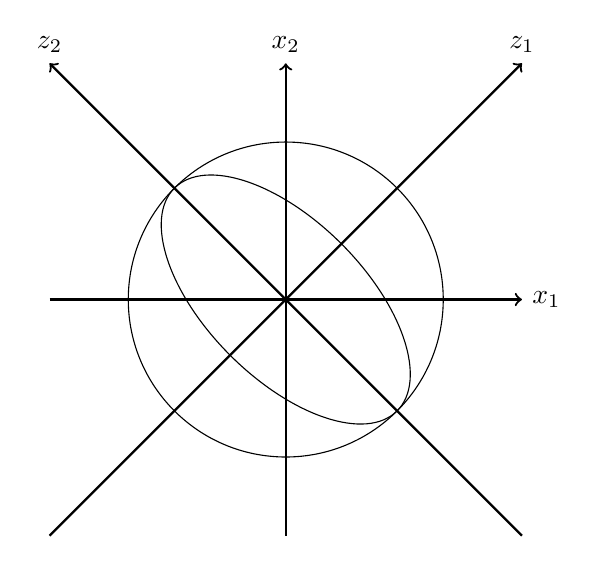
\begin{tikzpicture}
			\draw[->,thick] (-3,0) -- (3,0) node[right] {$x_1$};
			\draw[->,thick] (0,-3) -- (0,3) node[above] {$x_2$};
			\draw[rotate=-45] (0,0) ellipse (2cm and 1cm);
			\draw (0,0) circle (2);
			\draw[->,thick] (-3,-3) -- (3,3) node[above] {$z_1$};
			\draw[->,thick] (3,-3) -- (-3,3) node[above] {$z_2$};
		\end{tikzpicture}
	\end{center}
\end{example}

\begin{conclusion}
	\proplbl{6_7_5}
	Zu jeder hermiteschen Sesquilinearform $s$ auf $V$ gibt es eine Basis $B$ von $V$, für die 
	\begin{align}
		M_B(s)=\begin{pmatrix}\mathbbm{1_{r_{+}(s)}}&\;&\;\\\;&-\mathbbm{1_{r_{-}(s)}}&\;\\\;&\;&0\end{pmatrix}\notag
	\end{align}
	mit $r_+(s)+r_-(s)\le n$.
\end{conclusion}
\begin{proof}
	Sei $B_0=(x_1,...,x_n)$ eine Orthonormalbasis von $V$ mit $A=M_{B_0}(s)=\diag(\lambda_1,...,\lambda_n)$. Setze 
	\begin{align}
		\mu_i=
		\begin{cases}
			\frac{1}{\sqrt{\vert\lambda_i\vert}} & \lambda_i\neq 0 \\
			1 & \lambda_i=0
		\end{cases}\notag
	\end{align}
	Sei $x_i'=\mu_i\cdot x_i$ und $B'=(x'_1,...,x'_n)$. Dann ist $M_B(s)=S^tA\overline{S}$ mit $S=T^{B'}_{B_0}=\diag(\mu_1,...,\mu_n)$ also $M_{B'}(s)=\diag(\lambda'_1,...,\lambda'_n)$ mit $\lambda'_i=\mu_i\cdot \lambda_i\cdot\overline{\mu_i}=\mu_i^2\lambda_i\in\{0,1,-1\}$. Durch Permutation der Elemente von $B'$ erhält man die gewünschte Basis $B$.
\end{proof}

\begin{definition}[Ausartungsraum]
	Der \begriff{Ausartungsraum} von $s$ ist
	\begin{align}
		V_0=\{x\in V\mid s(x,y)=0\quad\forall y\in V\}\notag
	\end{align}
\end{definition}

\begin{lemma}
	$V_0$ ist ein Untervektorraum von $V$.
\end{lemma}
\begin{proof}
	Klar aus Linearität im ersten Argument.
\end{proof}

\begin{lemma}
	\proplbl{6_7_8}
	Seien $V_+$ und $V_-$ Untervektorräume von $V$ mit $V=V_+\oplus V_-\oplus V_0$ und $s$ positiv definit auf $V_+$, $-s$ positiv definit auf $V_-$. Dann ist
	\begin{align}
		\dim_K(V_+)&=\max\{\dim_K(W)\mid \text{Untervektorraum von }V,s\text{ positiv definit auf }V\}\notag \\
		\dim_K(V_-)&=\max\{\dim_K(W)\mid \text{Untervektorraum von }V,-s\text{ positiv definit auf }V\}\notag
	\end{align}
\end{lemma}
\begin{proof}
	Beweis nur für $V_+$, analog für $V_-$. \\
	$\le$: klar \\
	$\ge$: Ist $W\le V$ Untervektorraum mit $s(x,x)>0\quad\forall x\in W\backslash\{0\}$, so ist $W\cap(V_-\oplus V_+)=\{0\}$. Ist $x=y+z$ mit $y\in V_-$, $z\in V_0$, so ist $s(x,x)=s(y+z,y+z)=\underbrace{s(y,y)}_{\le 0}+\underbrace{s(y,z)+s(z,y)+s(z,z)}_{=0}\le 0\Rightarrow \dim_K(W)\le \dim_K(V)-\dim_K(V_-)-\dim_K(V_0)=\dim_K(V_+)$.
\end{proof}

\begin{theorem}[Trägheitssatz von \person{Sylvester}]
	Für eine hermitesche Sesquilinearform $s$ auf $V$ sind die Zahlen $r_+(s)$, $r_-(s)$ aus \propref{6_7_5} eindeutig bestimmt.
\end{theorem}
\begin{proof}
	Sei $B$ eine Basis von $V$ wie in \propref{6_7_5}, $B=(x_1,...,x_n)$. Definiere
	\begin{align}
		V_+&=\Span_K(x_1,...,x_{r_+(s)})\notag \\
		V_-&=\Span_K(x_{r_+(s)+1},...,x_{r_+(s)+r_-(s)})\notag \\
		V'_0&=\Span_K(x_{r_+(s)+r_-(s)+1},...,x_n)\notag
	\end{align}
	Dann ist $s$ positiv definit auf $V_+$, $-s$ positiv definit auf $V_-$ und $V=V_+\oplus V_-\oplus V'_0$. Es gilt $V'_0=V_0$\\
	$\subseteq$: klar \\
	$\supseteq$: Ist $x=\sum_{i=1}^{n} \lambda_ix_i\in V_0$, so ist $0=s(x,x_i)=\lambda_i\cdot s(x_i,x_i)$ für $i=1,...,n$ also $\lambda_i=0$ für $i=1,...,r_+(s)+r_-(s)$, d.h. $x\in V'_0$. Nach \propref{6_7_8} ist $r_+(s)=\dim_K(V_+)$ nur von $s$ abhängig, analog für $r_-(s)$.
\end{proof}

\begin{definition}[Signatur]
	Die \begriff{Signatur} von $s$ ist das Tripel
	\begin{align}
		(r_+(s),r_-(s),r_0(s))\notag
	\end{align}
	wobei $r_0(s)=\dim_K(V_0)$.
\end{definition}

\begin{conclusion}
	Ist $s$ eine hermitesche Form auf $V$ und $B$ eine Basis von $V$, so ist die Zahl der positiven bzw. negativen Eigenwerte von $M_B(s)$ gleich $r_+(s)$ bzw. $r_-(s)$, insbesondere also unabhängig von $B$.
\end{conclusion}
\begin{proof}
	Sei $A=M_B(s)$. Nach \propref{6_7_1} gibt es $S\in\Uni_n(K)$ mit $S^*AS$ eine reelle Diagonalmatrix. Da $S^*=S^{-1}$ haben $A$ und $S^*AS$ die selben Eigenwerte. Bringt man $S^*AS$ nun in die Form in \propref{6_7_5}, so ändern sich die Vorzeichen der Diagonale nicht mehr.
\end{proof}
\section{Quadriken}

Sei $n\in\natur$.

\begin{definition}[Quadrik]
	\proplbl{2_8_1}
	Eine \begriff{Quadrik} ist eine Teilmenge von $\real^n$ mit
	\begin{align}
		Q=\{x\in\real^n\mid x^tAx+2b^tx+c=0\}\notag
	\end{align}
	mit $A\in\Mat_n(\real)$ symmetrisch, $b^t\in\real^n$ und $c\in\real$.
\end{definition}

\begin{remark}
	\begin{itemize}
		\item $Q=\{x\in\real^n\mid \sum_{i,j=1}^n a_{ij}x_iy_j+2\sum_{i=1}^n b_ix_i+c=0\}$ also $Q$ ist die Nullstellenmenge eines quadratischen Polynoms in $x_1,...,x_n$
		\item $Q$ bestimmt $A,b,c$ nicht eindeutig, da $Q(A,b,c)=Q(\lambda A,\lambda b,\lambda c)$
		\item Man kann $A,b,c$ so normieren, dass $c=0$ oder $c=1$
	\end{itemize}
\end{remark}

\begin{remark}
	Seien $A,b,c$ wie in \propref{2_8_1}, so schreiben wir
	\begin{align}
		\tilde{A}&=\begin{pmatrix}A&b\\b^t&c\end{pmatrix}\notag \\
		\tilde{x}&=\begin{henrysmatrix}x\\1\end{henrysmatrix}\notag
	\end{align}
	Dann ist $Q=\{x\in\real^n\mid \tilde{x}^t\tilde{A}\tilde{x}=0\}$. Wir schreiben $(A,b)$ für 
	\begin{align}
		\begin{pmatrix}A&b\end{pmatrix}\in\Mat_{n,n+1}(\real)\notag
	\end{align}
	Es gilt $\rk(A)\le \rk(\tilde{A})$.
\end{remark}

\begin{remark}[Wiederholung]
	Seien $V,W$ $K$-Vektorräume. $f:V\to W$ heißt affin, wenn $\exists g\in\Hom_K(V,W)$ mit $f(v)=g(v)+w_0$ $\forall v\in V$. Ist $f$ affin und bijektiv, so ist $f^{-1}$ affin, d.h. $\Aff_K(V)=\{f:V\to V\mid f\text{ affin und bijektiv}\}$. Im Fall von $V=\real^n$, $K=\real$ ist
	\begin{align}
		\Aff_{\real}(\real^n)=\{f=\tau_z\circ f_T\mid T\in\GL_n(\real),z\in\real^n\}\notag
	\end{align}
	mit $f_T(x)=Tx$ und $\tau_z(x)=x+z$.
\end{remark}

\begin{lemma}
	Ist $Q\subseteq\real^n$ eine Quadrik, so ist $f(Q)$ eine Quadrik, für $f\in\Aff_{\real}(\real^n)$.
\end{lemma}
\begin{proof}
	$f=\tau_z\circ f_T$ mit $T\in\GL_n(\real)$ und $z\in\real^n$. Schreibe $S=T^{-1}\in\GL_n(\real)$, $\tilde{S}=\begin{henrysmatrix}S&0\\0&1\end{henrysmatrix}$. Es gilt $\tilde{S}\tilde{x}=\widetilde{Sx}$.
	\begin{align}
		f_T(Q)&=\{Tx\in\real^n\mid \tilde{x}^t\tilde{A}\tilde{x}=0\}\notag \\
		&=\{y\in\real^n\mid (\tilde{S}\tilde{y})^t\tilde{A}\tilde{S}\tilde{y}=0\}\notag \\
		&=\{y\in\real^n\mid \tilde{y}^t\underbrace{\tilde{S}^t\tilde{A}\tilde{S}}_{\begin{pmatrix}S^tAS&S^tb\\b^tS&c\end{pmatrix}}\tilde{y}=0\}\notag
	\end{align}
	Jetzt für $\tau_z$. Sei $U_z=\begin{henrysmatrix}\mathbbm{1}&z\\0&1\end{henrysmatrix}$. $U_z\tilde{x}=\tilde{\tau}_z(x)$. Man folgert analog, dass 
	\begin{align}
		\tau_z(Q)=\{y\in\real^n\mid \tilde{y}^t\underbrace{U_z^t\tilde{A}U_z}_{\begin{pmatrix} A&Az+b\\z^tA+b&z^tAz+b^tz+z^tb+c\end{pmatrix}}\tilde{y}=0\}\notag
	\end{align}
\end{proof}

\begin{definition}[Typen von Quadriken]
	Sei $Q$ gegeben durch $(A,b,c)$ wie in \propref{2_8_1}. $Q$ heißt
	\begin{itemize}
		\item vom \begriff[Quadrik!]{kegeligen Typ}, wenn $\rk(A)=\rk(A,b)=\rk(\tilde{A})$
		\item eine \begriff[Quadrik!]{Mittelpunktsquadrik}, wenn $\rk(A)=\rk(A,b)<\rk(\tilde{A})$
		\item vom \begriff[Quadrik!]{parabolischen Typ}, wenn $\rk(A)<\rk(A,b)$
	\end{itemize}
\end{definition}

\begin{lemma}
	Ist $Q\subseteq\real^n$ eine Quadrik, $f\in\Aff_{\real}(\real^n)$. Von dem Typ, von dem $Q$ ist, ist auch $f(Q)$.
\end{lemma}
\begin{proof}
	$f=f_{S^{-1}}$, $S\in\GL_n(\real)$. Da $\tilde{S}$ invertierbar ist, ist $\rk(\tilde{A})= \rk(\tilde{S}^t\tilde{A}\tilde{S})$, analog auch $\rk(S^tAS)=\rk(A)$. \\
	$(S^tAS,S^tb)=S^t(A,b)\begin{henrysmatrix}S&0\\0&1\end{henrysmatrix}\Rightarrow \rk(S^tAS,S^tb)=\rk(A,b)$. Für $f=\tau_z$ analog.
\end{proof}

\begin{definition}[Isometrie]
	Eine \begriff{Isometrie} des $\real^n$ ist $f\in\Aff_{\real}(\real^n)$ mit
	\begin{align}
		f(x)=Ax+b\notag
	\end{align}
	mit $b\in\real^n$ und $A\in\GL_n(\real)$ ist orthogonal.
\end{definition}

\begin{remark}
	$f:\real^n\to\real^n$ ist eine Isometrie genau dann, wenn $\Vert f(x)-f(y)\Vert=\Vert x-y\Vert$ für alle $x,y\in\real^n.$
\end{remark}

\begin{theorem}[Klassifikation bis auf Isometrien]
	Sei $Q$ eine Quadrik. Es gibt eine Isometrie $f\in\Aff_{\real}(\real^n)$ mit $f(Q)$, die eine der folgenden Formen annimmt:
	\begin{itemize}
		\item \itemEq{f(Q)=\left\lbrace x\in\real^n\mid \sum_{i=1}^k \left( \frac{x_i}{a_i}\right)^2 -\sum_{i=k+1}^{n} \left( \frac{x_i}{a_i}\right)^2=0\right\rbrace \quad k\ge r-k\notag}
		\item \itemEq{f(Q)=\left\lbrace x\in\real^n\mid \sum_{i=1}^k \left( \frac{x_i}{a_i}\right)^2 -\sum_{i=k+1}^{n} \left( \frac{x_i}{a_i}\right)^2=1\right\rbrace\notag}
		\item \itemEq{f(Q)=\left\lbrace x\in\real^n\mid \sum_{i=1}^k \left( \frac{x_i}{a_i}\right)^2 -\sum_{i=k+1}^{n} \left( \frac{x_i}{a_i}\right)^2-2x_{r+1}=0\right\rbrace \quad k\ge r-k, r<n\notag}
	\end{itemize}
	mit $a_1,...,a_r\in\real_{>0}$ und $0\le k\le r\le n$
\end{theorem}
\begin{proof}
	
\end{proof}

\begin{example}
	\proplbl{2_8_example}
	$Q\subseteq\real^2$
	\begin{itemize}
		\item \begin{itemize}
			\item \itemEq{k=2,r=2:\left\lbrace x\in\real^2\mid \left( \frac{x_1}{a_1}\right)^2+\left( \frac{x_2}{a_2}\right)^2=0\right\rbrace\notag}
			\begin{center}
				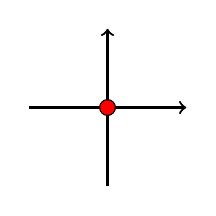
\begin{tikzpicture}
					\draw[->,thick] (-1,0) -- (1,0);
					\draw[->,thick] (0,-1) -- (0,1);
					\draw[fill=red] (0,0) circle (0.1);
				\end{tikzpicture}
			\end{center}
			\item \itemEq{k=1,r=2:\left\lbrace x\in\real^2\mid \left( \frac{x_1}{a_1}\right)^2-\left( \frac{x_2}{a_2}\right)^2=0\right\rbrace\notag}
			\begin{center}
				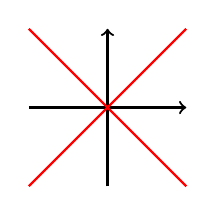
\begin{tikzpicture}
				\draw[->,thick] (-1,0) -- (1,0);
				\draw[->,thick] (0,-1) -- (0,1);
				\draw[thick, red] (-1,-1) -- (1,1);
				\draw[thick, red] (-1,1) -- (1,-1);
				\end{tikzpicture}
			\end{center}
			\item \itemEq{k=1,r=1:\left\lbrace x\in\real^2\mid \left( \frac{x_1}{a_1}\right)^2=0\right\rbrace\notag}
			\begin{center}
				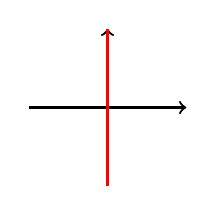
\begin{tikzpicture}
				\draw[->,thick] (-1,0) -- (1,0);
				\draw[->,thick] (0,-1) -- (0,1);
				\draw[thick, red] (0,-1) -- (0,1);
				\end{tikzpicture}
			\end{center}
		\end{itemize}
		\item \begin{itemize}
			\item\itemEq{k=2,r=2:\left\lbrace x\in\real^2\mid \left( \frac{x_1}{a_1}\right)^2+\left( \frac{x_2}{a_2}\right)^2=1 \right\rbrace\notag}
			\begin{center}
				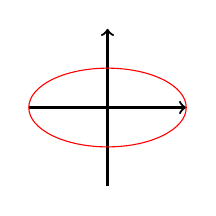
\begin{tikzpicture}
					\draw[->,thick] (-1,0) -- (1,0);
					\draw[->,thick] (0,-1) -- (0,1);
					\draw[red] (0,0) ellipse (1cm and 0.5cm);
				\end{tikzpicture}
			\end{center}
			\item\itemEq{k=1,r=2:\left\lbrace x\in\real^2\mid \left( \frac{x_1}{a_1}\right)^2-\left( \frac{x_2}{a_2}\right)^2=1 \right\rbrace\notag}
			\begin{center}
				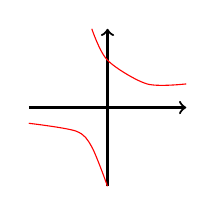
\begin{tikzpicture}
					\draw[->,thick] (-1,0) -- (1,0);
					\draw[->,thick] (0,-1) -- (0,1);
					\draw[red] plot [smooth] coordinates {(-0.2,1) (0,0.6) (0.5,0.3) (1,0.3)};
					\draw[red] plot [smooth] coordinates {(-1,-0.2) (-0.4,-0.3) (-0.2,-0.5) (0,-1)};
				\end{tikzpicture}
			\end{center}
			\item\itemEq{k=1,r=1:\left\lbrace x\in\real^2\mid \left( \frac{x_1}{a_1}\right)^2=1 \right\rbrace\notag}
			\begin{center}
				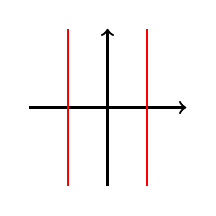
\begin{tikzpicture}
				\draw[->,thick] (-1,0) -- (1,0);
				\draw[->,thick] (0,-1) -- (0,1);
				\draw[thick, red] (-0.5,-1) -- (-0.5,1);
				\draw[thick, red] (0.5,-1) -- (0.5,1);
				\end{tikzpicture}
			\end{center}
			\item\itemEq{k=0,r=2:\left\lbrace x\in\real^2\mid -\left( \frac{x_1}{a_1}\right)^2-\left( \frac{x_2}{a_2}\right)^2=1 \right\rbrace=\emptyset\notag}
			\item\itemEq{k=0,r=1:\left\lbrace x\in\real^2\mid -\left( \frac{x_1}{a_1}\right)^2-\left( \frac{x_2}{a_2}\right)^2=1 \right\rbrace=\emptyset\notag}
		\end{itemize}
		\item \begin{itemize}
			\item\itemEq{k=1,r=1:\left\lbrace x\in\real^2\mid \left( \frac{x_1}{a_1}\right)^2-2x_2=0 \right\rbrace \notag}
			\begin{center}
				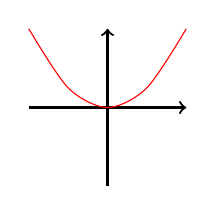
\begin{tikzpicture}
					\draw[->,thick] (-1,0) -- (1,0);
					\draw[->,thick] (0,-1) -- (0,1);
					\draw[red] plot [smooth] coordinates {(-1,1) (-0.5,0.25) (0,0) (0.5,0.25) (1,1)};
				\end{tikzpicture}
			\end{center}
		\end{itemize}
	\end{itemize}
\end{example}

\begin{remark}
	\begin{itemize}
		\item Ist $Q\subseteq\real^2$ eine Quadrik, $U\subseteq V$ affiner Untervektorraum, so ist $Q\cap U$ eine Quadrik in dem Sinne, dass $\exists f\text{ Isometrie}: f(U)=\real^k$ und $f(Q\cap U)$ ist eine Quadrik.
		\item Ebene Quadriken sind im wesentlichen Kegelschnitte, $Q'=\{x\in\real^3\mid x_1^2+x_2^2=x_3^2\}$, außer 2c und 2d in \propref{2_8_example}
	\end{itemize}
\end{remark}

\begin{conclusion}
	Sei $Q$ eine Quadrik, dann existiert eine lineare affine Abbildung $f$ mit: $f(Q)$ ist vom Typ 1, 2 oder 3.
\end{conclusion}

\begin{remark}
	$\real^n$ und "'Punkte im Unendlichen"' $\to \mathbb{P}^n(\real^n)$, der \begriff{projektive Raum}
\end{remark}


\chapter{Dualität}
\section{Das Lemma von Zorn}

Sei $K$ ein Körper und $U,V,W$ seien $K$-Vektorräume. Zudem sei $X$ eine Menge.

\begin{definition}[Relation]
	Eine \begriff{Relation} ist eine Teilmenge $R\subseteq X\times X$. Man schreibt $(x,x')\in R$ als $xRx'$. $R$ heißt
	\begin{itemize}
		\item \begriff[Relation!]{reflexiv}, wenn $\forall  x\in X$: $xRx$
		\item \begriff[Relation!]{transitiv}, wenn $\forall x,y,z\in X$: $xRy$ und $yRz\Rightarrow xRz$
		\item \begriff[Relation!]{symmetrisch}, wenn $\forall x,y\in X$: $xRy\Rightarrow yRx$
		\item \begriff[Relation!]{antisymmetrisch}, wenn $\forall x,y\in X$: $xRy$ und $yRx\Rightarrow y=x$
		\item \begriff[Relation!]{total}, wenn $\forall x,y\in X$: $(x,y)\notin R\Rightarrow (y,x)\in R$
	\end{itemize}
\end{definition}

\begin{example}[Äquivalenzrelation]
	Eine \begriff{Äquivalenzrelation} ist eine reflexive, transitive und symmetrische Relation. Wir haben schon verschiedene Äquivalenzrelationen kennengelernt: Isomorphie von $K$-Vektorräumen und Ähnlichkeit von Matrizen.
\end{example}

\begin{definition}[Halbordnung]
	Eine \begriff{Halbordnung} (oder \begriff{partielle Ordnung}) ist eine reflexive, transitive und antisymmetrische Relation $\le$. Eine totale Halbordnung heißt \begriff{Totalordnung} oder \begriff{lineare Ordnung}. Man schreibt $x<y$ für $x\le y\land x\neq y$.
\end{definition}

\begin{example}
	\begin{itemize}
		\item Die natürliche Ordnung $\le$ auf $\real$, $\ratio$, $\whole$ und $\natur$ ist eine Z
		Totalordnung.
		\item Teilbarkeit $\vert$ ist eine Halbordnung auf $\natur$, aber Teilbarkeit ist keine Halbordnung auf $\whole$, da $1\vert -1$ und $-1\vert 1$, aber $1\neq -1$!
		\item $\mathcal{P}(X)$ ist die Potenzmenge. "$\subseteq$" ist eine Halbordnung auf $\mathcal{P}$, aber für $\vert X\vert>1$ ist "$\subseteq$" keine Totalordnung.
		\item Sei $(X,\le)$ eine Halbordnung, sei $Y\subseteq X$, so ist $(Y,\subseteq\vert_Y)$ eine Halbordnung.
	\end{itemize}
\end{example}

\begin{definition}[Kette]
	Sei $(X,\le)$ eine Halbordnung, $Y\subseteq X$. $Y$ heißt \begriff{Kette}, wenn $(Y,\le\vert_Y)$ total ist.
	
	$x\in Y$ heißt ein \begriff[Kette!]{minimales Element} von $Y$, wenn $\forall x'\in Y$: $x<x'$.
	
	$x\in Y$ heißt \begriff[Kette!]{untere Schranke} von $Y$, wenn $\forall y\in Y$: $y\ge x$.
	
	$x\in Y$ heißt \begriff[Kette!]{kleinstes Element} von $Y$, wenn $x$ untere Schranke von $Y$ ist.
	
	Analog: \begriff[Kette!]{maximales Element}, \begriff[Kette!]{obere Schranke}, \begriff[Kette!]{größtes Element}.
\end{definition}

\begin{center}
	\begin{tikzpicture}
		\node[place] (A) {1};
		\node[place] (B) [below=of A] {3};
		\node[place] (C) [left=of B] {2};
		\node[place] (D) [right=of B] {5};
		\node[place] (E) [right=of D] {7};
		\node[place] (dots) [right=of E] {...};
		
		\node[place] (F) [below=of C] {4};
		\node[place] (G) [below=of B] {6};
		\node[place] (H) [below=of E] {15};
		\node[place] (I) [right=of G] {10};
		\node[place] (dots2) [right=of H] {...};
		
		\node[place] (J) [below=of F] {8};
		\node[place] (K) [below=of J] {16};
		\node[place] (L) [below=of K] {32};
		
		\draw[->,thick] (A.west) -- (C.north);
		\draw[->,thick] (A.south) -- (B.north);
		\draw[->,thick] (A.east) -- (D.north);
		\draw[->,thick] (A.east) -- (E.north);
		\draw[->,thick] (A.east) -- (dots.north);
		
		\draw[->,thick] (C.south) -- (F.north);
		\draw[->,thick] (C.south) -- (G.north);
		\draw[->,thick] (B.south) -- (G.north);
		\draw[->,thick] (C.south) -- (I.north);
		\draw[->,thick] (D.south) -- (I.north);
		\draw[->,thick] (B.south) -- (H.north);
		\draw[->,thick] (D.south) -- (H.north);
		\draw[->,thick] (E.south) -- (dots2.north);
		\draw[->,thick] (D.south) -- (dots2.north);
		
		\draw[->,thick] (F.south) -- (J.north);
		\draw[->,thick] (J.south) -- (K.north);
		\draw[->,thick] (K.south) -- (L.north);
	\end{tikzpicture}
	$Y=\{2^n\mid n\in\natur\}$ ist eine Kette
\end{center}

\begin{remark}
	\begin{itemize}
		\item Hat $Y$ ein kleinstes Element, so ist dies eindeutig bestimmt. Ein kleinstes Element ist minimal.
		\item Jede endliche Halbordnung hat minimale Elemente. Jede endliche Totalordnung hat ein kleinstes Element. Analog für maximale Elemente und größtes Element.
	\end{itemize}
\end{remark}

\begin{example}
	$(\natur,\le)$ hat als kleinstes Element die 1, aber kein größtes Element oder maximale Elemente.
\end{example}

\begin{example}
	$V=\real^3$, $\mathfrak{X}$ die Menge der Untervektorräume des $\real^3$. $(\mathfrak{X},\le)$ ist eine Halbordnung auf $Y\subseteq X$ mit $Y=\{U\in\mathfrak{X}\mid \dim_\real(U)\le 2\}$. 
	\begin{itemize}
		\item $Y$ hat ein kleinstes Element: $\{0\}$.
		\item Es gibt unendlich viele maximale Elemente in $Y$, nämlich die Untervektorräume von $V$, die die Dimension 2 haben. Es gibt also kein größtes Element.
		\item $V$ ist die obere Schranke von $Y$.
	\end{itemize}
\end{example}

\begin{theorem}[Das Lemma von Zorn]
	Sei $(X,\le)$ eine Halbordnung, die nicht leer ist. Wenn jede Kette eine obere Schranke hat, dann hat $X$ ein maximales Element.
\end{theorem}
\begin{proof}
	Das Lemma von Zorn hat axiomatischen Charakter - es ist äquivalent zum Auswahlaxiom, seine Gültigkeit ist somit abhängig von unseren grundlegenden mengentheoretischen Annahmen. Für einen Beweis des Lemmas von Zorn aus dem Auswahlaxiom siehe die Vorlesung \textit{Mengenlehre}. Wir zeigen hier zumindest die andere Richtung, nämlich dass das Auswahlaxiom aus dem Lemma von Zorn folgt.
\end{proof}

\begin{conclusion}[Auswahlaxiom]
	Zu jeder Familie $(x_i)$, nicht leer, gibt es eine \begriff{Auswahlfunktion}, das heißt eine Abbildung:
	\begin{align}
		f: I\to \bigcup_{i\in I} X_i\text{ mit } f(i)\in X_i\quad\forall i\notag
	\end{align}
\end{conclusion}
\begin{proof}
	Sei $\mathcal{F}$ die Menge der Paare $(J,f)$ bestehend aus einer Teilmenge $J\subseteq I$ und einer Abbildung $f:I\to \bigcup_{i\in I} X_i$ mit $f(i)\in X_i\quad\forall i\in J$. Definieren wir $(J,f)\le (J',f')\iff J\subseteq J'$ und $f'\vert_J = f$, so ist $\le$ eine Halbordnung auf $\mathcal{F}$. Da $(\emptyset,\emptyset)\in\mathcal{F}$ ist $\mathcal{F}$ nichtleer. Ist $\mathcal{G}\subseteq\mathcal{F}$ eine nichtleere Kette, so wird auf $J':=\bigcup_{(J,f)\in\mathcal{G}} J$ durch $f'(j)=f(j)$ falls $(J,f)\in\mathcal{G}$ und $j\in J$ eine wohldefinierte Abbildung $f':J\to \bigcup_{i\in J}X_i$ mit $f'(i)\in X_i\quad\forall i\in J'$ gegeben. Das Paar $(J',f')$ ist eine obere Schranke der Kette $\mathcal{G}$. Nach dem Lemma von Zorn besitzt $\mathcal{F}$ ein maximales Element $(J,f)$. Wir behaupten, dass $J=I$. Andernfalls nehmen wir ein $i'\in I\backslash J$ und ein $x'\in X_{i'}$ und definieren $J':= U\cup\{i'\}$ und $f':J'\to \bigcup_{i\in J'} X_i$, $j\mapsto\begin{cases}f(j)&j\in J\\ x'&j=i'\end{cases}$. Dann ist $(J',f')\in\mathcal{F}$ und $(J,f)<(J',f')$ im Widerspruch zur Maximalität von $(J,f)$.
\end{proof}


\begin{conclusion}[Basisergänzungssatz]
	\proplbl{3_1_11}
	Sei $V$ ein $K$-Vektorraum. Jede linear unabhängige Teilmenge $X_0\subseteq V$ ist in einer Basis von $V$ enthalten.
\end{conclusion}
\begin{proof}
	Sei $\mathfrak{X}=\{X\subseteq V\mid X\text{ ist linear unabhängig, } X_0\subseteq X\}$ geordnet durch Inklusion. Dann ist $X_0\in\mathfrak{X}$, also $\mathfrak{X}\neq\emptyset$. Ist $\mathcal{Y}$ eine nichtleere Kette in $\mathfrak{X}$, so ist auch $Y=\bigcup\mathcal{Y}\subseteq V$ linear unabhängig. Sind $y_1,...,y_n\in Y$ paarweise verschieden, so gibt es $Y_1,...,Y_n\in\mathcal{Y}$ mit $y_i\in Y_i$ für $i=1,...,n$. Da $\mathcal{Y}$ total geordnet ist, besitzt $\{Y_1,...,Y_n\}$ ein größtes Element, o.E. $Y_1$. Also sind $y_1,...,y_n\in Y_1$ und somit linear unabhängig. Folglich ist $Y_1\in \mathfrak{X}$ eine obere Schranke von $\mathcal{Y}$. Nach dem Lemma von Zorn besitzt $\mathfrak{X}$ ein maximales Element $X$. Das heißt, $X$ ist eine maximal linear unabhängige Teilmenge von $V$, nach LAAG1 II.3.5 also eine Basis von $V$. %TODO: Verlinkung
	\end{proof}
\section{Der Dualraum}

Sei $V$ ein $K$-Vektorraum.

\begin{definition}[Dualraum]
	Der \begriff{Dualraum} zu $V$ ist der $K$-Vektorraum
	\begin{align}
		V^*=\Hom_K(V,K)=\{\phi:V\to K\text{ linear}\}\notag
	\end{align}
	Die Elemente von $V^*$ heißen \begriff{Linearformen} auf $V$.
\end{definition}

\begin{example}
	Ist $V=K^n=\Mat_{n\times 1}(K)$, so wird $V^*=\Hom_K(V,K)$ durch $\Mat_{1\times n}(K)\cong K^n$. Wir können also die Elemente von $V$ als Spaltenvektoren und die Linearformen auf $V$ als Zeilenvektoren auffassen.
\end{example}

\begin{lemma}
	Ist $B(x_1)_{i\in I}$ eine Basis von $V$, so gibt es zu jedem $i\in I$ genau $x_i^*\in V^*$ mit 
	\begin{align}
		x_i^*(x_j)=\delta_{ij}\quad\forall j\in I\notag
	\end{align}
\end{lemma}
\begin{proof}
	Siehe LAAG1 III.5.1, angewandt auf die Familie $(y_j)_{j\in I}$, $y_j\delta_{i.j}$ in $W=K$. %TODO: Verlinkung
\end{proof}

\begin{proposition}
	Ist $B=(x_1)_{i\in I}$ eine Basis von $V$, so ist $B^*=(x_i^*)_{i\in I}$ linear unabhängig. Ist $I$ endlich, so ist $B^*$ eine Basis von $V^*$.
\end{proposition}
\begin{proof}
	Ist $\phi=\sum_{i\in I} \lambda_ix_i^*$, $\lambda_i\in K$, fast alle gleich 0, so ist $\phi(x_j)=\sum_{i\in I} \lambda_j x_i^*(x_j)=\lambda_j$ für jedes $j\in I$. Ist also $\phi=0$, so ist $\lambda_j=\phi(x_j)=0\quad\forall j\in I$, $B^*$ ist somit linear unabhängig. \\
	Ist zudem $I$ endlich und $\psi\in V^*$, so ist $\psi=\psi'=\sum_{i\in I} \psi(x_i)x_i^*$, denn $\psi'(x_j)=\sum_{i\in I} \psi(x_i)x_i^*(x_j)=\psi(x_i)\quad\forall j\in I$, und somit ist $B^*$ ein Erzeugendensystem von $V^*$.
\end{proof}

\begin{definition}[duale Basis]
	Ist $B=(x_i)_{i\in I}$ eine endliche Basis von $V$, so nennt man $B^*=(x_i^*)_{i\in I}$ die zu $B$ \begriff{duale Basis}.
\end{definition}

\begin{conclusion}
	\proplbl{3_2_6}
	Zu jeder Basis $B$ von $V$ gibt es einen eindeutig bestimmtem Monomorphismus
	\begin{align}
		f_V\to V^*\text{ mit } f(B)=B^*\notag
	\end{align}
	Ist $\dim_K(V)<\infty$, so ist dieser ein Isomorphismus.
\end{conclusion}

\begin{conclusion}
	\proplbl{3_2_7}
	Zu jedem $=0\neq x\in V$ gibt es eine Linearform $\phi\in V$ mit $\phi(x)=1$.
\end{conclusion}
\begin{proof}
	Ergänze $x_1=x$ zu einer Basis $(x_i)_{i\in I}$ von $V$ (\propref{3_1_11}) und $\phi=x_1^*$.
\end{proof}

\begin{example}
	Ist $V=K^n$ mit Standardbasis $\mathcal{E}=(e_1,...,e_n)$, so können wir $V^*$ mit dem Vektorraum der Zeilenvektoren identifizieren, und dann ist
	\begin{align}
		e_i^* = e_i^t\notag
	\end{align}
\end{example}

\begin{definition}[Bidualraum]
	Der \begriff{Bidualraum} zu $V$ ist der $K$-Vektorraum
	\begin{align}
		V^{**}=(V^*)^*=\Hom_K(V^*,K)\notag
	\end{align}
\end{definition}

\begin{proposition}
	Die kanonische Abbildung
	\begin{align}
		\iota:\begin{cases}
		V\to V^{**} \\ x\to \iota_x
		\end{cases}\text{ wobei } \iota_x(\phi)=\phi(x)\notag
	\end{align}
	ist ein Monomorphismus. Ist $\dim_K(V)<\infty$, so ist $\iota$ ein Isomorphismus.
\end{proposition}
\begin{proof}
	\begin{itemize}
		\item $\iota_x\in V^{**}$: 
		\begin{itemize}
			\item $\iota_x(\phi+\psi)=(\phi+\psi)(x)=\phi(x)+\psi(x)=\iota_x(\phi)+ \iota_x(\psi)$
			\item $\iota_x(\lambda \phi)=(\lambda\phi)(x)=\lambda\phi(x)=\lambda\iota_x(\phi)$
		\end{itemize}
		\item $\iota$ linear: 
		\begin{itemize}
			\item $\iota_{x+y}(\phi)=\phi(x+y)=\phi(x)+\phi(y)=\iota_x(\phi)+\iota_y(\phi)= (\iota_x+\iota_y)(\phi)$
			\item $\iota_{\lambda x}(\phi)=\phi(\lambda x)=\lambda\iota_x(\iota)=(\lambda\iota_x)(\phi)$
		\end{itemize}
		\item $\iota$ injektiv: Sei $0\neq x\in V$. Nach \propref{3_2_7} existiert $\phi\in V^*$ mit $\iota_x(\phi)=\phi(x)=1\neq 0$. Somit ist $\iota_x\neq 0$.
		\item Ist $\dim_K(V)<\infty$, so ist $V\overset{\propref{3_2_6}}{\cong} V^* \overset{\propref{3_2_6}}{\cong} V^{**}$, insbesondere $\dim_K(V)=\dim_K(V^{**})$. Der Monomorphismus $\iota$ ist somit ein Isomorphismus.
	\end{itemize}
\end{proof}

\begin{remark}
	Sei $\dim_K(V)<\infty$. Im Gegensatz zu den Isomorphismen $V\to V^*$, die von der Wahl der Basis $B$ abhängen, ist der Isomorphismus $\iota:V\to V^{**}$ kanonisch (von der Wahl der Basis $B$ unabhängig).
	
	Die Voraussetzung, dass $\dim_K(V)<\infty$ ist hier essentiell: Für $\dim_K(V)=\infty$ ist $\iota$ nicht surjektiv.
\end{remark}

\begin{definition}[Annulator]
	Für eine Teilmenge $U\subseteq V$ bezeichne
	\begin{align}
		U^0 =\{\phi\in V^*\mid \phi(x)=0\quad\forall x\in U\}\notag
	\end{align}
	den \begriff{Annulator} von $U$.
\end{definition}

\begin{lemma}
	$U^0$ ist ein Untervektorraum von $V^*$.
\end{lemma}
\begin{proof}
	Klar.
\end{proof}

\begin{proposition}
	\proplbl{3_2_14}
	Ist $\dim_K(V)<\infty$ und $U\subseteq V$ ein Untervektorraum, so ist
	\begin{align}
		\dim_K(V)=\dim_K(U)+\dim_K(U^0)\notag
	\end{align}
\end{proposition}
\begin{proof}
	Ergänze eine Basis $(x_1,...,x_r)$ von $U$ zu einer Basis $B=(x_1,...,x_n)$ von $V$. Dann ist $B^*(x_1^*,...,x_n^*)$ eine Basis von $V^*$. Sei $C=(x_{r+1}^*,...,x_n^*)$. Dann ist $C$ eine Basis von $U^0$: 
	\begin{itemize}
		\item $B^*$ ist Basis $\Rightarrow C$ ist linear unabhängig.
		\item $C\subseteq U^0$: Für $1\le j\le r < i\le n$ ist $x_i^*(x_j)=\delta_{ij}=0$.
		\item $U^0\subseteq\Span_K(C)$: Ist $\phi=\sum_{i=1}^n \lambda_ix_i^*\in U^0$, so $0=\phi(x_j)= \lambda_j$ für alle $j\le r$, \\also $\phi\in\Span_K(x_{r+1}^*,...,x_n^*)$.
	\end{itemize}
\end{proof}

\begin{conclusion}
	\proplbl{3_2_15}
	Ist $\dim_K(V)<\infty$ und $U\subset V$ ein Untervektorraum, so ist
	\begin{align}
		\iota(U)=U^{00}\notag
	\end{align}
\end{conclusion}
\begin{proof}
	Es ist klar, dass $\iota(U)\le U^{00}$. \\
	Für $\phi\in U^0$ und $x\in U$ ist $\iota_x(\phi) = \phi(x) =0$. Mit \propref{3_2_14} ist
	\begin{align}
		\dim_K(U^{00}) &= \dim_K(V^*)-\dim_K(U^0) \notag \\
		&=\dim_K(V^*) - (\dim_K(V)-\dim_K(U)) \notag \\
		&\overset{\propref{3_2_6}}{=} \dim_K(U) \notag
	\end{align}
	und da $\iota$ injektiv ist, folgt $\iota(U)=U^{00}$.
\end{proof}
\section{Die duale Abbildung}

Sei $f\in\Hom_K(V,W)$.

\begin{definition}[duale Abbildung]
	Die zu $f$ duale Abbildung ist
	\begin{align}
		f^*:
		\begin{cases}
			W^*\to V^* \\
			\phi\mapsto \phi\circ f
		\end{cases} \notag
	\end{align}
\end{definition}
\section{Die adjungierte Abbildung}

Sei $K=\real$ oder $K=\comp$ und $V$ ein endlichdimensionaler unitärer $K$-Vektorraum.

\begin{definition}[weitere Skalarmultiplikation]
	Wir definieren auf $V$ eine Skalarmultiplikation
	\begin{align}
		\lambda\ast x=\overline{\lambda}\cdot x\notag
	\end{align}
	und schreiben $\overline{V}=(V,+,\ast)$.
\end{definition}

\begin{lemma}
	$\overline{V}$ ist ein $K$-Vektorraum und $\End_K(V)=\End_K(\overline{V})$.
\end{lemma}
\begin{proof}
	Mit LAAG1 VI.1.7 nachprüfen, zum Beispiel:
	\begin{itemize}
		\item $\lambda\ast (x+y)=\overline{\lambda}\cdot (x+y)=\overline{\lambda} x+\overline{\lambda} y=\lambda\ast x+\lambda\ast y$
		\item $\lambda\ast(\mu\ast x)=\overline{\lambda}(\overline{\mu}\cdot x)=\overline{\lambda\mu}x=(\lambda\mu)\ast x$
	\end{itemize}
	Weiterhin sei: $f\in\End_K(V)$, $x\in V$, $\lambda\in K$ \\
	$\Rightarrow f(\lambda\ast x)=f(\overline{\lambda}x)=\lambda\ast f(x)$ \\
	$\Rightarrow f\in \End_K(\overline{V})$. \\
	Umgekehrt sei $g\in\End_K(\overline{V})$, $x\in V$, $\lambda\in K$ \\
	$\Rightarrow g(\lambda\cdot x)=g(\overline{\lambda}\ast x)=\lambda\cdot g(x)$ \\
	$\Rightarrow g\in \End_K(V)$. \\
\end{proof}

\begin{lemma}
	Für $y\in V$ ist
	\begin{align}
		\Phi_y:
		\begin{cases}
			V\to K \\ x\mapsto\skalar{x}{y}
		\end{cases}\notag
	\end{align}
	eine Linearform auf $V$.
	
	Die Abbildung $y\mapsto\Phi_y$ liefert einen Isomorphismus $\Phi:\overline{V}\to V^*$.
\end{lemma}
\begin{proof}
	\begin{itemize}
		\item $\Phi_y\in V^*$: Linearität in ersten Argument.
		\item $\Phi\in \Hom_K(\overline{V},V^*)$: Für $y,y'\in V$, $\lambda\in K$, $x\in V$ ist
		\begin{itemize}
			\item $\Phi_{y+y'}(x)=\skalar{x}{y+y'}=\skalar{x}{y}+\skalar{x}{y'}=\Phi_y(x)+\Phi_{y'}(x)$
			\item $\Phi_{\lambda\ast y}(x)=\skalar{x}{\lambda\ast x}=\skalar{x}{\overline{\lambda}y}=\lambda \skalar{x}{y}=\lambda\Phi_y(x)$
		\end{itemize}
		\item $\Phi$ injektiv: Skalarprodukt ist nicht ausgeartet.
		\item Da $\dim_K(\overline{V})=\dim_K(V)=\dim_K(V^*)$ ist $\Phi$ somit ein Isomorphismus.
	\end{itemize}
\end{proof}

\begin{proposition}
	Zu $f\in\End_K(V)$ gibt es ein eindeutig bestimmtes $f^{adj}\in\End_K(V)$ mit 
	\begin{align}
		\skalar{f(x)}{y}=\skalar{x}{f^{adj}(y)}\quad\forall x,y\in V\notag
	\end{align}
\end{proposition}
\begin{proof}
	Existenz und Eindeutigkeit sind zu zeigen.
	\begin{itemize}
		\item Existenz:
		\begin{center}
			\begin{tikzcd}
				\overline{V} \arrow[r, "f"] \arrow[d, "\Phi"]
				& \overline{V} \arrow[d, "\Phi"] \arrow[l, "f^{adj}"] \\
				V^{\ast}
				& V^{\ast} \arrow[l, "f^*"]
			\end{tikzcd}
		\end{center} %TODO: Ändern
		Für $f^{adj}=\Phi{-1}\circ f^*\circ \Phi\in \End_K(\overline{V})=\End_K(V)$ ist 
		\begin{align}
			\Phi_y\circ = (f^*\circ \Phi)(y)=(\Phi\circ f^{adj.})(y)=\Phi_{f^{adj}(y)}\notag
		\end{align}
		also
		\begin{align}
			\skalar{f(x)}{y}=(\Phi_y\circ f)(x)=\Phi_{f^{adj}(y)}(x)=\skalar{x}{f^{adj}(y)}\quad\forall x,y\in V\notag
		\end{align}
		\item Eindeutigkeit: Erfüllen $f_1,f_2$ für Gleichung
		\begin{align}
			\skalar{f(x)}{y}=\skalar{x}{f^{adj}(y)}\quad\forall x,y\in V\notag
		\end{align}
		so ist
		\begin{align}
			0=\skalar{x}{f_1(y)}-\skalar{x}{f_2(y)}=\skalar{x}{f_1(y),f_2(y)}\quad\forall x,y\in V\notag
		\end{align}
		da $\skalar{\cdot}{\cdot}$ nicht ausgeartet ist, folgt daraus, dass $f_1=f_2$.
	\end{itemize}
\end{proof}

\begin{definition}[adjungierter Endomorphismus]
	Die Abbildung $f^{adj}$ heißt der zu $f$ \begriff[Endomorphismus!]{adjungierte Endomorphismus}.
\end{definition}

\begin{example}
	\begin{itemize}
		\item Ist $f$ selbstadjungiert, so ist $f^{adj}=f$.
		\item Ist $f$ unitär, so ist $f\in\Aut_K(V)$ und 
		\begin{align}
		\skalar{f(x)}{y}=\skalar{x}{f^{-1}(y)}\quad\forall x,y\in V\notag
		\end{align}
		also $f^{adj}=f^{-1}$.
	\end{itemize}
\end{example}

\begin{lemma}
	\proplbl{3_4_7}
	Ist $B$ eine Orthonormalbasis vin $V$, so ist
	\begin{align}
		M_B(f^{adj})=M_B(f^*)\notag
	\end{align}
\end{lemma}
\begin{proof}
	Ist $A=M_B(f)$ und $B=M_B(f^{adj})$, $v=\Phi_B(x)$, $w=\Phi_B(y)$, so ist
	\begin{align}
		(Ax)^t\overline{y}=\skalar{f(v)}{w}&=\skalar{v}{f^{adj}(w)}\notag \\
		x^tA^t\overline{y} &= x^t\overline{B}\overline{y} \notag \\
		\Rightarrow B&= \overline{A^t}=A^*\notag
	\end{align}
\end{proof}

\begin{lemma}
	\proplbl{3_4_8}
	Für $f,g\in\End_K(V)$ und $\lambda,\mu\in K$ ist
	\begin{align}
		(\lambda f+\mu g)^{adj} &= \overline{\lambda}f^{adj}+\overline{\mu}g^{adj}\notag \\
		(f^{adj})^{adj} &= f\notag
	\end{align}
\end{lemma}
\begin{proof}
	Für $x,y\in V$ ist
	\begin{align}
		\skalar{(\lambda f+\mu g)(x)}{y}&=\lambda\skalar{f(x)}{y}+\mu\skalar{g(x)}{y}\notag \\
		&= \lambda\skalar{x}{f^{adj}(y)}+\mu\skalar{x}{g^{adj}} \notag \\
		&= \skalar{x}{(\overline{\lambda}f^{adj}+\overline{\mu}g^{adj})(y)}\notag
	\end{align}
	und
	\begin{align}
		\skalar{f^{adj}(x)}{y}=\overline{\skalar{y}{f^{adj}(y)}}=\overline{\skalar{f(y)}{x}}=\skalar{x}{f(y)}\notag
	\end{align}
\end{proof}
\section{Der Spektralsatz}

Sei $V$ ein endlichdimensionaler unitärer $K$-Vektorraum und $f\in\End_K(V)$.

\begin{definition}[normaler Endomorphismus, normale Matrix]
	Der Endomorphismus $f$ heißt \begriff[Endomorphismus!]{normal}, wenn
	\begin{align}
		f\circ f^{adj}=f^{adj}\circ f\notag
	\end{align}
	
	Entsprechend heißt $A\in\Mat_n(K)$ \begriff[Matrix!]{normal}, wenn
	\begin{align}
		AA^*=A^*A\notag
	\end{align}
\end{definition}

\begin{example}
	\begin{itemize}
		\item Ist $f$ selbstadjungiert, so ist $f^{adj}=f$, insbesondere ist $f$ normal.
		\item Ist $f$ unitär, so ist $f^{adj}=f^{-1}$, insbesondere ist $f$ normal.
	\end{itemize}
\end{example}

\begin{lemma}
	\proplbl{3_5_3}
	Genau dann ist $f\in\End_K(V)$ normal, wenn
	\begin{align}
		\skalar{f(x)}{f(y)}=\skalar{f^{adj}(x)}{f^{adj}(y)}\quad\forall x,y\in V\notag
	\end{align}
\end{lemma}
\begin{proof}
	\begin{itemize}
		\item Hinrichtung: Ist $f$ normal, so ist
		\begin{align}
			\skalar{f(x)}{f(y)} &= \skalar{x}{(f^{adj}\circ f)(y)} \notag \\
			&= \skalar{x}{(f\circ f^{adj})(y)} \notag \\
			&= \skalar{f^{adj}(x)}{f^{adj}(y)}\quad\forall x,y\in V\notag
		\end{align}
		\item Rückrichtung: Ist umgekehrt $\skalar{f^{adj}(x)}{f^{adj}(y)}$, so ist
		\begin{align}
			\skalar{x}{(f^{adj}\circ f)(y)}&=\skalar{x}{(f\circ f^{adj})(y)} \notag \\
			0 &= \skalar{x}{(f^{adj}\circ f-f\circ f^{adj})(y)} \notag \\
			f^{adj}\circ f&=f\circ f^{adj} \notag
		\end{align}
	\end{itemize}
\end{proof}

\begin{lemma}
	\proplbl{3_5_4}
	Ist $f$ normal, ist ist
	\begin{align}
		\Ker(f)=\Ker(f^{adj})\notag
	\end{align}
\end{lemma}
\begin{proof}
	Nach \propref{3_5_3} ist
	\begin{align}
		\Vert f(x)\Vert = \Vert f^{adj}(x)\Vert \quad\forall x\in V\notag
	\end{align}
	Insbesondere gilt
	\begin{align}
		f(x)=0\iff f^{adj}(x)=0\notag
	\end{align}
\end{proof}

\begin{lemma}
	\propref{3_5_5} %TODO fix reference
	Ist $f$ normal, so ist
	\begin{align}
		\Eig(f,\lambda)=\Eig(f^{adj},\overline{\lambda})\quad\forall\lambda\in K\notag
	\end{align}
\end{lemma}
\begin{proof}
	Da $(\lambda\cdot \id-f)^{adj}\overset{\propref{3_4_8}}{=}\overline{\lambda}\cdot\id-f^{adj}$ ist auch $\lambda\cdot\id-f$ normal. Somit ist
	\begin{align}
		\Eig(f,\lambda) &= \Ker(\lambda\id-f)\notag \\
		&\overset{\propref{3_5_4}}{=} \Ker((\lambda\id-f)^{adj})\notag \\
		&= \Ker(\overline{\lambda}\id-f^{adj})\notag \\
		&= \Eig(f^{adj},\overline{\lambda})\notag
	\end{align}
\end{proof}

\begin{theorem}[Spektralsatz]
	\proplbl{3_5_6}
	Sei $f\in\End_K(V)$ ein Endomorphismus, für den $\chi_f$ in Linearfaktoren zerfällt. Genau dann besitzt $V$ eine Orthonormalbasis aus Eigenvektoren von $f$, wenn $f$ normal ist.
\end{theorem}
\begin{proof}
	\begin{itemize}
		\item Hinrichtung: Ist $B$ eine Orthonormalbasis aus Eigenvektoren von $f$, so ist $A=M_B(f)$ eine Diagonalmatrix. Dann ist auch $M_B(f^{adj})\overset{\propref{3_4_7}}{=}A^*$ eine Diagonalmatrix und $AA^*=A ^*A$. Somit ist $f$ normal.
		\item Rückrichtung: Sei $f$ normal und $\chi_f(t)=\prod_{i=1}^n (t-\lambda_i)$. Beweis nach Induktion nach $n=\dim_K(V)$. \\
		\emph{$n=0$}: klar \\
		\emph{$n-1\to n$}: Wähle Eigenvektor zum Eigenwert $\lambda_1$, o.E. $\Vert x_1\Vert = 1$. Sei $U=K\cdot x_1$. Nach \propref{3_5_5} ist $f^{adj}(x_1)=\overline{\lambda_1}x_1$, insbesondere ist $U$ $f$-invariant und $f^{adj}$-invariant. Für $x\in U^\perp$ ist 
		\begin{align}
			\skalar{f(x)}{x_1}= \skalar{x}{f^{adj}(x_1)}=\skalar{x}{\overline{\lambda_1}x_1}=\lambda_1\skalar{x}{x_1}=0\notag
		\end{align}
		also $f(x)\in U^\perp$ und 
		\begin{align}
			\skalar{f^{adj}(x)}{x_1}=\skalar{x}{f(x_1)}=\skalar{x}{\lambda_1 x_1}=\overline{\lambda_1} \skalar{x}{x_1}=0\notag
		\end{align}
		also $f^{adj}(x)\in U^\perp$. Somit ist $V=U\oplus U^\perp$ eine Zerlegung in Untervektorräume, die sowohl $f$-invariant als auch $f^{adj}$-invariant sind. Insbesondere st $f^{adj}\vert_{U^\perp}=(f\vert_{U^\perp})^{adj}$, woraus folgt, dass auch $f\vert_{U^\perp}$ normal ist:
		\begin{align}
			f\vert_{U^\perp}\circ (f\vert_{U^\perp})^{adj}=f\circ f^{adj}\vert_{U^\perp}=f^{adj}\circ f\vert_{U^\perp} = f^{adj}\vert_{U^\perp}\circ f\vert_{U^\perp}=(f\vert_{U^\perp})^{adj}\circ f\vert_{U^\perp}\notag
		\end{align}
		Außerdem zerfällt auch $\chi_{f\vert_{U^\perp}}=\prod_{i=2}^n (t-\lambda_i)$ in Linearfaktoren. Nach Induktionshypothese existiert eine Orthonormalbasis $(x_2,...,x_n)$ von $U^\perp$ bestehend aus Eigenvektoren von $f\vert_{U^\perp}$ und $(x_1,...,x_n)$ ist dann eine Orthonormalbasis von $V$ aus Eigenvektoren von $f$.
	\end{itemize}
\end{proof}

\begin{conclusion}
	Sei $A\in\Mat_n(\comp)$. Genau dann gibt es $S\in\Uni_n$ mit $S^*AS=D$ eine Diagonalmatrix, wenn $A$ normal ist.
\end{conclusion}

\begin{remark}
	\propref{3_5_6} ist eine gemeinsame Verallgemeinerung von \propref{2_5_9} und \propref{2_6_5}
\end{remark}
\section{Tensorprodukte}

\begin{definition}[billineare Abbildung]
	Eine Abbildung $\xi:V\times W\to U$ ist \begriff[Abbildung!]{bilinear}, wenn für jedes $v\in V$ die Abbildung 
	\begin{align}
		\begin{cases}
		W\to U \\ w\mapsto \xi(v,w)
		\end{cases}\notag
	\end{align}
	und für jedes $w\in W$ die Abbildung
	\begin{align}
	\begin{cases}
	V\to U \\ v\mapsto \xi(v,w)
	\end{cases}\notag
	\end{align}
	linear sind.
	
	Wir definieren
	\begin{align}
		\Bil_K(V,W,U)=\{\xi\in\Abb(V\times W,U)\mid \xi\text{ bilinear}\}\notag
	\end{align}
\end{definition}

\begin{example}
	Seien $V=W=K[t]_{\le d}$, $U=K[t]_{\le 2d}$. Die Abbildung
	\begin{align}
	\xi:\begin{cases}
	V\times W\to U \\ (f.g)\mapsto fg
	\end{cases}\quad\text{ ist bilinear}\notag
	\end{align}
	Wir sehen, dass $\Image(\xi)$ im Allgemeinen kein Untervektorraum von $U$ ist. Ist zum Beispiel $K=\ratio$, $d=1$, so liegen $t^2=\xi(t,t)$ und $-2=\xi(-2,1)$ im $\Image(\xi)$ nicht jedoch $t^2-2$, denn wäre $t^2-2=fg$ mit $f,g\in\ratio[t]$ linear, so hätte $t^2-2$ eine Nullstelle in $\ratio$, aber $\sqrt{2}\notin\ratio$.
\end{example}

\begin{lemma}
	$\Bil_K(V,W,U)$ bildet einen Untervektorraum des $K$-Vektorraum $\Abb(V\times W,U)$.
\end{lemma}
\begin{proof}
	klar, zum Beispiel
	\begin{align}
		(\xi+\xi')(\lambda v,w)=\xi(\lambda v,w)+\xi'(\lambda v,w)=\lambda\xi(v,w)+\lambda\xi(v,w)= \lambda(\xi+\xi')(v,w)\notag
	\end{align}
\end{proof}

\begin{lemma}
	Ist $\xi\in\Bil_K(V,W,U)$ und $f\in\Hom_K(U,U')$ für einen $K$-Vektorraum, so ist 
	\begin{align}
		f\circ \xi\in\Bil_K(V,W,U')\notag
	\end{align}
\end{lemma}
\begin{proof}
	klar, zum Beispiel
	\begin{align}
		(f\circ\xi)(\lambda v,w)=f(\xi(\lambda v,w))=f(\lambda\xi(v,w))=\lambda\cdot(f\circ\xi)(v,w)\notag
	\end{align}
\end{proof}

\begin{lemma}
	\proplbl{3_6_5}
	Sei $(v_i)_{i\in I}$ eine Basis von $V$ und $(w_j)_{j\in J}$ eine Basis von $W$. Zu jeder Familie $(u_{ij})_{(i,j)\in I\times J}$ in $U$ gibt es genau ein $\xi\in\Bil_K(V,W,U)$ mit
	\begin{align}
		\xi(v_i,w_i)=u_{ij}\quad\forall i\in I, j\in J\notag
	\end{align}
\end{lemma}
\begin{proof}
	\begin{itemize}
		\item Eindeutigkeit: Ist $\xi$ bilinear, $v=\sum_{i\in I} \lambda_i v_i$, $w=\sum_{j\in J} \mu_j w_j$ so ist 
		\begin{align}
			\xi(v,w)&=\xi\left(\sum_{i\in I} \lambda_i v_i,\sum_{j\in J}\mu_j w_j\right) \notag \\
			&= \sum_{i\in I}\lambda_i\xi\left(v_i,\sum_{j\in J}\mu_j w_j\right)\notag \\
			&= \sum_{i,j}\lambda_i\mu_j u_{ij}
		\end{align}
		durch die Familie $(u_{ij})_{i,j}$ bestimmt.
		\item Existenz: Wird $\xi$ durch (1) definiert, so ist $\xi$ bilinear: Für festes $w=\sum_{j\in J}\mu_j w_j$ ist
		\begin{align}
			\begin{cases}
			V&\to U \\ v=\sum\limits_{i\in I}\lambda_i v_i&\mapsto \xi(v,w)=\sum\limits_{i\in I}\lambda_i\left(\sum\limits_{j\in J}\mu_j u_{ij}\right)
			\end{cases}\notag
		\end{align}
		linear (LAAG1 III.5.1), analog für festes $v$. %TODO: Verlinkung
	\end{itemize}
\end{proof}

\begin{definition}[Tensorprodukt]
	Ein \begriff{Tensorprodukt} von $V$ und $W$ ist ein Paar $(T,\tau)$ bestehend aus einem $K$-Vektorraum $T$ und einer bilinearen Abbildung $\tau\in\Bil_K(V,W,T)$ welche die folgende \begriff{universelle Eigenschaft} erfüllt: \\
	\textit{Ist $U$ ein weiterer $K$-Vektorraum und $\xi\in\Bil_K(V,W,U)$ so gibt es genau ein $\xi_\otimes\in\Hom_K(T,U)$ mit $\xi=\xi_\otimes\circ\tau$.}
	\begin{center}
		\begin{tikzpicture}
		\matrix (m) [matrix of math nodes,row sep=3em,column sep=4em,minimum width=2em]
		{V\times W & T \\ \; & U \\};
		\path[-stealth]
		(m-1-1) edge node [below] {$\xi$} (m-2-2)
		edge node [above] {$\tau$} (m-1-2)
		(m-1-2) edge [dashed] node [right] {$\xi_\otimes$} (m-2-2);
		\end{tikzpicture}
	\end{center}
\end{definition}

\begin{*anmerkung}
	Sind $V$ und $W$ zwei Vektorräume und $K$ ein gemeinsamer Körper, so kann man das Tensorprodukt $V\otimes W$, was auch ein Vektorraum ist, wie folgt konstruieren: Wenn $B=(b_1,...,b_n)$ eine Basis von $V$ und $C=(c_1,...,c_m)$ eine Basis von $W$ ist, dass ist $V\otimes W$ ein Vektorraum, genannt \textit{Tensorproduktraum}, in dem es eine Basis gibt, die auf eindeutige Weise mit den geordneten Paaren des kartesischen Produkts
	\begin{align}
		B\times C=\{(b_i,c_j)\}\notag
	\end{align}
	der Basen der Ausgangsräume identifiziert werden kann. Die Dimension von $V\otimes W$ ist dann das Produkt der Dimensionen von $V$ und $W$. Ein Element der Basis von $V\otimes W$, das dem Paar $(b_i,c_j)$ entspricht, wird als $b_i\otimes c_j$ notiert, das $\otimes$ hat also keine tiefere Bedeutung. Ein Element des Tensorproduktes $V\otimes W$ hat dann die Gestalt:
	\begin{align}
		\sum_{i,j} \lambda_{ij}\cdot (b_i\otimes c_j)\notag
	\end{align}
	mit $\lambda_{ij}\in K$.
\end{*anmerkung}

\begin{lemma}
	\proplbl{3_6_7}
	Sind $(T,\tau)$ und $(T',\tau')$ Tensorprodukte von $V$ und $W$, so gibt es einen eindeutig bestimmten Isomorphismus $\Theta:T\to T'$ mit $\tau'=\Theta\circ\tau$.
	\begin{center}
		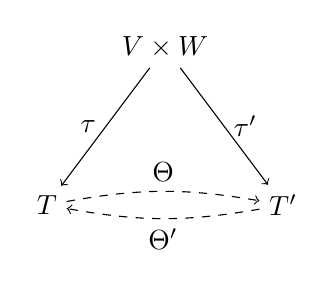
\begin{tikzpicture}
		\node (V) at (1.5,0) {$V\times W$};
		\node (T) at (0,-2) {$T$};
		\node (S) at (3,-2) {$T'$};
		\draw[->, left] (V) to node {$\tau$} (T);
		\draw[->, right] (V)  to node {$\tau'$} (S);
		\draw[->, above, dashed] (T)  to [bend left=10] node {$\Theta$} (S);
		\draw[->, below, dashed] (S)  to [bend left=10] node {$\Theta'$} (T);
		\end{tikzpicture}
	\end{center}
\end{lemma}
\begin{proof}
	Da $(T,\tau)$ die universelle Eigenschaft erfüllt, gibt es ein eindeutig bestimmtes $\Theta=(\tau')_\otimes\in\Hom_K(T,T')$ mit $\tau'=\Theta\circ\tau$. Analog gibt es $\Theta'\in\Hom_K(T',T)$ mit $\tau=\Theta'\circ\tau'$. Es folgt, dass $\tau=\Theta'\circ\tau'= \Theta'\circ\Theta\circ\tau$. Da auch $\tau=\id_T\circ\tau$ liefert die Eindeutigkeitsaussage in der universellen Eigenschaft von $(T,\tau)$, für $U=T$, $\xi=\tau$, dass $\Theta\circ\Theta'=\id_T$. Analog sieht man, dass $\Theta\circ\Theta'=\id_{T'}$. Somit ist $\Theta$ ein Isomorphismus.
\end{proof}

\begin{definition}[Vektorraum mit Basis $X$]
	\proplbl{3_6_8}
	Sei $X$ eine Menge. Der $K$-\begriff{Vektorraum mit Basis $X$} ist der Untervektorraum $V=\Span_K((\delta_x)_{x\in X})$ des $K$-Vektorraum $\Abb(X,K)$ mit $\delta_x(y)=\delta_{x,y}=\begin{cases}1&x=y\\0&x\neq y\end{cases}$
\end{definition}

\begin{lemma}
	Sei $X$ eine Menge und $V$ der $K$-Vektorraum mit Basis $X$. Dann ist $V$ ein $K$-Vektorraum und $(\delta_x)_{x\in X}$ ist eine Basis von $V$.
\end{lemma}
\begin{proof}
	Zu zeigen ist nur, dass $(\delta_x)_{x\in X}$ linear unabhängig ist. Ist $f=\sum_{x\in X}\lambda_x \delta_x$, $\lambda_x\in K$, fast alle gleich 0, und $f=0$, so ist $\lambda_x=f(x)=0$ für jedes $x\in X$. 
\end{proof}

\begin{lemma}
	\proplbl{3_6_10}
	Sei $(v_i)_{i\in I}$ eine Basis von $V$ und $(w_j)_{j\in J}$ eine Basis von $W$. Sei $T$ der $K$-Vektorraum mit der Basis $I\times J$ (im Sinne von \propref{3_6_8}) und $\tau:V\times W\to T$ die bilineare Abbildung gegeben durch $(v_i,w_j)\mapsto \delta_{i,j}$, vergleiche \propref{3_6_5}. Dann ist $(T,\tau)$ ein Tensorprodukt von $V$ und $W$.
\end{lemma}
\begin{proof}
	Wir schreiben $v_i\otimes w_j$ für $\delta_{i,j}$. Sei $U$ ein weiterer $K$-Vektorraum und $\xi\in\Bil_K(V,W,U)$. Da $(v_i\otimes w_j)_{(ij)\in I\times J}$ eine Basis von $T$ ist, gibt es genau ein $\xi_\otimes\in\Hom_K(T,U)$ mit $\xi_\otimes(v_i\otimes w_j)=\xi(v_i,w_j)$ für alle $i,j$, also mit $\xi_\otimes\circ\tau=\xi$ nach \propref{3_6_5}. Die universelle Eigenschaft ist somit erfüllt.
\end{proof}

\begin{proposition}
	Es gibt ein bis auf Isomorphie (im Sinne von \propref{3_6_7}) eindeutig bestimmtes Tensorprodukt
	\begin{align}
		(V\otimes_K W,\otimes)\notag
	\end{align}
	von $V$ und $W$. Sind $V$ und $W$ endlichdimensional, so ist
	\begin{align}
		\dim_K(V\otimes_K W)=\dim_K(V)\cdot\dim_K(W)\notag
	\end{align}
\end{proposition}
\begin{proof}
	\propref{3_6_10} und \propref{3_6_7}
\end{proof}

\begin{example}
	Durch die Wahl der Standardbasis erhält man einen kanonischen Isomorphismus $K^m\otimes_K K^n\cong\Mat_{m\times n}(K)$.
\end{example}

\begin{example}
	Ist $V$ ein $\real$-Vektorraum mit Basis $(x_1,...,x_n)$, so ist $\comp\otimes_\real V$ ein $\real$-Vektorraum der Dimension $2n$ mit Basis $(1\otimes x_1...,1\otimes x_n,i\otimes x_1,...,i\otimes x_n)$. Durch $\lambda\cdot z\otimes x=(\lambda z)\otimes x$ für $\lambda,z\in\comp$, $x\in V$ wird $\comp\otimes_\real V$ zu einem $\comp$-Vektorraum der Dimension $1\otimes x_1,...,1\otimes x_n$, $V_\comp$, genannt die \begriff{Komplexifizierung} von $V$.
\end{example}

\begin{proposition}
	\proplbl{3_6_14}
	Sei $V\otimes_K W$ ein Tensorprodukt von $V$ und $W$. Für jeden weiteren $K$-Vektorraum $U$ liefert die Abbildung $\xi\to\xi_\otimes$ ein Isomorphismus 
	\begin{align}
		\Bil_K(V,W,U)\overset{\cong}{\to}\Hom_K(V\otimes_K W,U)\notag
	\end{align}
\end{proposition}
\begin{proof}
	Diese Abbildung heiße $\Lambda$. 
	\begin{itemize}
		\item $\Lambda$ ist linear: klar aus Eindeutigkeitsaussage, z.B.
		\begin{align}
			(\xi_\otimes+\xi'_\otimes)\circ\otimes=\xi_\otimes\circ\otimes+\xi'_\otimes\circ\otimes=\xi+\xi'=(\xi+\xi')_\otimes\circ\otimes\notag
		\end{align}
		und somit $\xi_\otimes+\xi'_\otimes=(\xi+\xi')_\otimes$.
		\item $\Lambda$ ist injektiv: Ist $\xi\neq 0$, so wegen $\xi=\xi_\otimes\circ\otimes$ auch $\xi_\otimes\neq 0$.
		\item $\Lambda$ ist surjektiv: Ist $f\in\Hom_K(V\otimes_K W,U)$, so ist $\xi=f\circ\otimes$ bilinear, die universelle Eigenschaft liefert somit $f=\xi_\otimes\in\Image(\Lambda)$.
	\end{itemize}
\end{proof}

\begin{conclusion}
	Sind $V$ und $W$ endlichdimensional, so ist
	\begin{align}
		V\otimes_K W\cong \Bil_K(V,W,K)^*\notag
	\end{align}
\end{conclusion}
\begin{proof}
	Es ist $\dim_K(V\otimes_K W)<\infty$ und deshalb
	\begin{align}
		V\otimes_K W\cong (V\otimes_K W)^{**}\overset{\propref{3_6_14}}{\cong} \Bil_K(V,W,K)\notag
	\end{align}
\end{proof}

\begin{remark}
	Während obige Konstruktion des Tensorprodukts von der Wahl (und Existenz) von Basen abhängt, ist die folgende Konstruktion "'basisfrei"': \\
	Sei $T_1$ der $K$-Vektorraum mit Basis $V\times W$ und $T_0$ der Untervektorraum von $T_1$ erzeugt von Elementen der Form:
	\begin{align}
		\delta_{v+v',w}-\delta_{v,w}-\delta_{v',w} \notag \\
		\delta_{v,w+w'}-\delta_{v,w}-\delta_{v,w'} \notag \\
		\delta_{\lambda v,w}-\lambda\cdot \delta_{v,w} \notag \\
		\delta_{v,\lambda w}-\lambda\cdot\delta_{v,w}\notag
	\end{align}
	mit $v,v'\in V$, $w,w'\in W$ und $\lambda\in K$. Sei weiter $T=T_1/T_0$ und $\tau:V\times W\to T$ gegeben durch $(v,w)\mapsto\delta_{v,w}+T_0$. Dann ist $(T,\tau)$ ein Tensorprodukt von $V$ und $W$.
	\begin{center}
		\begin{tikzpicture}
		\node (K) at (0,0) {$V\times W$};
		\node (U) at (3,-2) {$U$};
		\node (B) at (3,0) {$T_1/T_0$};
		\node (T) at (3,2) {$T_1$};
		\draw[->, above] (K) to node {$\tau$} (B);
		\draw[->, below] (K)  to node {$\xi$} (U);
		\draw[->] (K) to node {} (T);
		\draw[->, right] (T) to node {$\pi_{\tau_0}$} (B);
		\draw[->, dashed] (B) to node {} (U);
		\draw[->, dashed] (T)  to [bend left=60] node {} (U);
		\end{tikzpicture}
	\end{center}
\end{remark}

\begin{remark}
	Analog kann man für $k\ge 2$ und die $K$-Vektorräume $V_1,...,V_k$ $k$-lineare Abbildungen $V_1\times ...\times V_k\to U$ definieren und erhält dann Tensorprodukte $V_1\otimes_K ... \otimes_K V_k$.
\end{remark}

\chapter{Moduln}
In diesem ganzen Kapitel sei $R$ ein kommutativer Ring mit Einselement.

\section{Moduln}

\begin{definition}
	Ein $R$-\begriff{Modul} ist ein Tripel $(M,+,\cdot)$ bestehend aus einer Menge $M$, einer Verknüpfung $+:M\times M\to M$ und der Abbildung $\cdot:R\times M\to M$ (Skalarmultiplikation) für die gelten:
	\begin{itemize}
		\item (M1): $(M,+)$ ist eine abelsche Gruppe
		\item (M2): Addition und Skalarmultiplikation sind verträglich. Für alle $x,y\in M$ und $a,b\in R$ gelten
		\begin{itemize}
			\item $a(x+y)=ax+ay$
			\item $(a+b)x=ax+bx$
			\item $a\cdot bx=ab\cdot x$
			\item $1\cdot x=x$
		\end{itemize}
	\end{itemize}
\end{definition}

\begin{example}
	\begin{itemize}
		\item Ist $R=K$ ein Körper, so sind die $R$-Moduln genau die $K$-Vektorräume.
		\item Ist $R=\whole$, so sind die $R$-Moduln genau die abelschen Gruppen mit der einzig möglichen Skalarmultiplikation 
		\begin{align}
			\whole\times A\to A,(k,a)\mapsto ka=\underbrace{1+...+1}_{k\text{-mal}}a=\underbrace{a+...+a}_{k\text{-mal}}\notag
		\end{align}
		vergleiche Laag 1 III.2.3 %TODO: Verlinkung
		\item Jedes Ideal $M\subseteq R$ ist ein $R$-Modul mit Einschränkung der Multiplikation als Skalarmultiplikation.
		\item Ist $K$ ein Körper, $V$ ein $K$-Vektorraum und $f\in\End_K(V)$, so wird $V$ durch $P(t)\cdot x:=P(f)(x)$ zu einem Modul über dem Ring $R=K[t]$, siehe auch V.5.2 %TODO: Verlinkung
	\end{itemize}
\end{example}

\begin{remark}
	Sei $M$ ein $R$-Modul. Wie für Vektorräume (LAAG 1 II.1.5) überzeugt man sich leicht, dass $0x=0$, $a0=0$, $(-a)x=a(-x)=-ax$ für alle $a\in R$, $x\in M$. 
	
	Im Gegensatz zu Vektorräumen folgt aber aus $ax=0$ nicht, dass $a=0$ oder $x=0$, siehe zum Beispiel das $\whole$-Modul $M=\whole/n\whole$. Es ist
	\begin{align}
		n\cdot\overline{1}=\overline{n}=\overline{0}\in\whole/n\whole\notag
	\end{align}
	aber $0\neq n\in\whole$.
\end{remark}

\begin{definition}[Homomorphismus von $R$-Moduln]
	Seien $M,M'$ $R$-Moduln. Eine Abbildung $f:M\to M'$ ein \begriff[Modul!]{Homomorphismus} von $R$-Moduln (oder $R$-Homomorphismus oder $R$-linear), wenn
	\begin{align}
		f(x+y)&=f(x)+f(y) \notag \\
		f(ax) &= a\cdot f(x)\notag
	\end{align}
	Wir bezeichnen die Menge der $R$-Homomorphismen $f:M\to M'$ mit $\Hom_R(M,M')$. Wie üblich definiert man den \begriff[Modul!]{Kern} eines $R$-Homomorphismus, sowie die Begriffe \begriff[Modul!]{Monomorphismus}, \begriff[Modul!]{Epimorphismus}, \begriff[Modul!]{Isomorphismus}, \begriff[Modul!]{Endomorphismus} und \begriff[Modul!]{Automorphismus} von $R$-Moduln.
\end{definition}

\begin{example}
	\begin{itemize}
		\item Ist $R=K$, so sind die $R$-Homomorphismen genau die lineare Abbildungen.
		\item Ist $R=\whole$, so sind die $R$-Homomorphismen genau die Gruppenhomomorphismen.
	\end{itemize}
\end{example}

\begin{example}
	Für jedes $a\in R$ ist die Abbildung
	\begin{align}
		\begin{cases}
		M\to M \\ x\mapsto ax
		\end{cases}\notag
	\end{align}
	einen Endomorphismus von $M$.
\end{example}

\begin{definition}[Untermodul, Erzeugendensystem]
	Ein \begriff{Untermodul} ist eine nichtleere Teilmenge $N\subseteq M$, für die gilt:
	\begin{itemize}
		\item Sind $x,y\in N$, so ist auch $x+y\in N$.
		\item Ist $a\in R$ und $x\in N$, so ist auch $ax\in N$.
	\end{itemize}

	Für eine Familie $(x_i)_{i\in I}$ ist
	\begin{align}
		\sum_{i\in I} Rx_i=\{\sum_{i\in I} ax_i\mid a\in R\text{, fast alle gleich 0}\}\notag
	\end{align}
	der von $(x_i)_{i\in I}$ \begriff[Untermodul!]{erzeugte Untermodul} von $M$. Ist $\sum_{i\in I} Rx_i=M$, so ist $(x_i)_{i\in I}$ ein \begriff[Modul!]{Erzeugendensystem} von $M$. Der $R$-Modul $M$ ist \begriff[Modul!]{endlich erzeugt}, wenn er ein endliches Erzeugendensystem besitzt.
\end{definition}

\begin{remark}
	Wieder ist der Kern eines $R$-Homomorphismus $f:M\to M'$ ein Untermodul von $M$. Leicht sieht man auch hier, dass $\sum_{i\in I} Rx_i$ ein Untermodul von $M$ ist, und zwar der kleinste, der alle $x_i$ enthält.
\end{remark}

\begin{example}
	\begin{itemize}
		\item Ist $R=K$ ein Körper, so sind die Untermoduln von $M$ genau die Untervektorräume.
		\item Ist $R=\whole$, so sind die Untermoduln von $M$ genau die Untergruppen und der von einer Familie erzeugte Untermodul ist genau gleich der davon erzeugten Untergruppe. \\
		Ist zum Beispiel $M=\whole$, so sind alle $n\whole$ Untermoduln von $M$.
	\end{itemize}
\end{example}

\begin{definition}[freie Familie, Basis]
	Eine Familie $(x_i)_{i\in I}$ in $M$ ist \begriff[Familie!]{frei} oder ($R$-linear unabhängig), wenn es keine Familie $(\lambda_i)_{i\in I}$ von Elementen von $R$, fast alle gleich 0, aber nicht alle gleich 0, mit $\sum_{i\in I} \lambda_ix_i=0$ gibt.
	
	Ein freies Erzeugendensystem heißt \begriff[Modul!]{Basis}. Besitzt $M$ eine Basis, so nennt man $M$ \begriff[Modul!]{frei}.
\end{definition}
\section{Teilbarkeit}

Sei $R$ ein \textbf{nullteilfreier} Ring.

\begin{definition}[teilt, assoziert, irreduzibel, prim, ggT, kgV]
	\proplbl{2_4_1}
	Seinen $x,y,z,p \in R$.
	\begin{enumerate}[label=(\alph*)]
		\item $x$ \begriff{teilt} $y$ (in Zeichen $x \mid y$) $\Leftrightarrow \exists z \in R: xz = y$
		\item $x$ ist \begriff{assoziert} zu $y$ (in Zeichen $x \sim y$) $\Leftrightarrow \exists z \in R^{\times}, xz = y$
		\item $p$ ist \begriff{irreduzibel} $\Leftrightarrow p \not \in R^{\times} \cup \{  0\}$ und $\forall x,y \in R$:
		\begin{align}
			p = xy &\Rightarrow x \in R^{\times} \text{ oder } y \in R^{\times} \notag
		\end{align}
		\item $p$ ist \begriff{prim} $\Leftrightarrow  p \not \in R^{\times} \cup \{ 0 \}$ und $\forall x,y \in R$:
		\begin{align}
			p \mid xy &\Rightarrow p \mid x \text{ oder } p \mid y \notag
		\end{align}
		\item $z$ ist \begriff{größter gemeinsamer Teiler} von $x,y$ (in Zeichen $z = \ggT(x,y)$) $\Leftrightarrow  z \mid x$ und $z \mid y$ und $\forall a \in R: a\mid x$ und $a \mid y\Rightarrow a \mid z$
		\item $z$ ist \begriff{kleinstes gemeinsames Vielfaches} von $x,y$ (in Zeichen $z = \kgV(x,y)$) $\Leftrightarrow x \mid z$ und $y \mid z$ und $\forall a \in R: x \mid a$ und $y \mid a \Rightarrow z \mid a$
	\end{enumerate}
\end{definition}

\begin{remark}
	\begin{enumerate}[label=(\alph*)]
		\item $x \mid y \Leftrightarrow y \in (x) \Leftrightarrow (y) \subseteq (x)$
		\item $x \sim y \Leftrightarrow x \mid y \text{ und } y \mid x \Leftrightarrow (x) = (y)$
		\item $p$ prim $\Leftrightarrow (p)$ prim und $p \neq 0$
		\item $p$ prim $\Rightarrow p$ irreduzibel
		\item Analog zu e) und f) in \propref{2_4_1} kann man ein $\ggT$ bzw. $\kgV$ von endlich vielen Elementen von $R$ definieren.
	\end{enumerate}
\end{remark}
\begin{proof}
	\begin{itemize}
		\item[d)] $p = xy \Rightarrow p \mid xy \xRightarrow{p \text{ prim}} p \mid x \text{ oder } p\mid y$, ohne Einschränkung $p \mid x$, das heißt $x = px'$ mit $x' \in R \Rightarrow p(1-x'y) =0 \Rightarrow 1 - x'y = 0 \Rightarrow 1 = x'y \Rightarrow y \in R^{\times}$
	\end{itemize}
\end{proof}

\begin{definition}[euklidisch, Hauptidealring, faktoriell]
	\begin{enumerate}[label=(\alph*)]
		\item $R$ ist \begriff{euklidisch} $\Leftrightarrow$ es gibt eine euklidische Gradfunktion:
		\begin{align}
			\delta: R\setminus \{0\} \to \natur_0 \notag
		\end{align}
		mit $\forall x,y \in R\setminus \{0\} \exists q,r \in R$ mit $x = qy + r$ und $r=0$ oder $\delta(r) < \delta(y)$
		\item $R$ ist \begriff{Hauptidelring} $\Leftrightarrow$ Jedes Ideal $I \unlhd R$ ist ein Hauptideal.
		\item $R$ ist \begriff{faktoriell} $\Leftrightarrow$ Jedes $0 \neq x \in R\setminus R^{\times}$ ist ein Produkt von Primelementen.
	\end{enumerate}
\end{definition}

\begin{proposition}
	$R$ euklidisch $\Rightarrow R$ Hauptidealring $\Rightarrow R$ faktoriell.
\end{proposition}

\begin{proof}
	LAAG VIII.3.6 und VIII.4.4.
\end{proof}

\begin{example}
	\begin{enumerate}[label=(\alph*)]
		\item $\whole$, $K[x]$: euklidisch
		\item $K$ Körper: euklidisch
		\item $\whole[i] = \{ a+b\sqrt{-1} \mid a,b \in \whole \} \subseteq \comp$: euklidisch mit $\delta(z) = \vert z \vert^2$
		\item $K[x,y], \whole[x]$: keine Hauptidealringe
		\item $\whole[\sqrt{-5}] = \{ a+b\sqrt{-5} \mid a,b \in \whole \} \subseteq \comp$: nicht faktoriell, da $6 = 2\cdot 3 = (1 + \sqrt{-5})(1-\sqrt{-5})$
	\end{enumerate}
\end{example}

\begin{remark}
	Ist $R$ faktoriell, so gilt:
	\begin{enumerate}[label=(\alph*)]
		\item $p$ irreduzibel $\Leftrightarrow p$ prim
		\item Eine Darstellung von $0 \neq x \in R \setminus R^{\times}$ als Produkt von Primelementen ist eindeutig bis auf Reihenfolge und Assoziiertheit.
	\end{enumerate}
\end{remark}

\begin{proposition}
	Sei $R$ ein Hauptidealring. Wenn $(0) \neq \mathfrak{p} \unlhd R$ ein Primideal ist, so ist $\mathfrak{p}$ maximal.
\end{proposition}

\begin{proof}
	Sei $\mathfrak{p} \subseteq I \unlhd R$. Da $R$ ein Hauptidealring ist, kann man $\mathfrak{p} = (p)$ mit $p \in R$ prim schreiben. $p$ ist prim, insbesondere irreduzibel. Weiterhin gilt $I = (a)$ mit $a \in R$ und $a \mid p$. Da $p$ prim, gilt $a \sim 1$ oder $a \sim p$. Also $I = R$ oder $I = \mathfrak{p}$. Damit ist $\mathfrak{p}$ maximal.
\end{proof}

\begin{remark}
	In jedem Hauptidealring gilt:
	\begin{align}
		(x) + (y) = (\ggT(x,y,)) \notag
	\end{align}
	anders gesagt
	\begin{align}
		\ggT(x,y) = ax + by \notag
	\end{align}
	mit $a,b \in R$. In euklidischen Ringen können $a$ und $b$ explizit bestimmt werden.
\end{remark}

\begin{proposition}[Erweiterter euklidischer Algorithmus]
	Sei $R$ euklidisch mit euklidischer Gradfunktion $\delta$, und seien $x,y \in R$. Man setze $x_0 = x, x_1 = y, b_0 = 0, a_1 = 0, b_1 = 1$ und berechne iterativ $x_{i+1}, q_{i+1}, a_{i+1}, b_{i+1}$ für $i \ge 1$ als
	\begin{align}
		x_{i-1} &= q_{i+1}x_i + x_{i+1} &\qquad &x_{i+1} = 0 \text{ oder } \delta(x_{i+1}) < \delta(x_i) \notag \\
		a_{i+1} &= a_{i-1} + q_{i+1}a_i & & \notag \\
		b_{i+1} = b_{i-1} - q_{i+1}b_i & & \notag
	\end{align}
	solange bis $x_{k+1} = 0$. Dann ist
	\begin{align}
		\ggT(x,y) = x_k = a_k x + b_k y \notag
	\end{align}
\end{proposition}

\begin{proof}
	Da $\delta(x_1) > \delta(x_2) > \dots >$ wird $x_{k+1} = 0$ irgendwann erreicht. Für jedes $i \le k$ ist 
	\begin{align}
		\ggT(x_{i-1}, x_i) &= \ggT(q_{i+1}x_i + x_{i+1}, x_i)\notag \\
		&=\ggT(x_{i+1}, x_i) \notag \\
		&= \ggT(x_i, x_{i+1}) \notag
	\end{align}
	somit im Allgemeinen:
	\begin{align}
		\ggT(x,y) &= \ggT(x_0,x_1) = \ggT(x_0,x_1) = \dots = \ggT(x_k, \underbrace{x_{k+1}}_{=0})\notag \\
		&= x_k \notag
	\end{align}
	Per Induktion sieht man, dass $x_i = a_i x + b_i y$ für alle \\
	$i \le k: x_{i-1} = a_{i-1} x + b_{i-1}y, x_i = a_i x + b_i y$ sowie\\
	$x_{i-1} = q_{i+1 x_i + x_{i+1}}$\\
	\begin{align}
	\Rightarrow x_{i-1} &= x_{i-1}q_{i+1}x_i = (a_{i+1} - q_{i+1} q_i)x + (b_{i-1}-q_{i+1}b_i)y \notag\\
	&= a_{i+1}x + b_{i+1}y\notag
	\end{align}
\end{proof}

\begin{example}
	$R = \whole, x = 5, y= 13$
	\begin{align}
	5 &= 0\cdot 13 + 5 \notag \\
	13 &= 2\cdot 5 + 3 \notag \\
	5 &= 1\cdot 3 + 2 \notag \\
	3 &= 1\cdot 2 + 1 \notag \\
	5 &= 2\cdot \underline{1} + 0 \notag \\
	\end{align}
	$\Rightarrow \ggT(5,13) = 1 = 2\cdot 13 - 5 \cdot 5$ %TODO somewhere here is an error!
\end{example}

\begin{example}
	Bestimme $x \in \whole$ mit $x \in 1 \mod 5$ und $x \equiv 2 \mod 13$.\\
	$b_1 = 2 \cdot 13 = 26$
	\begin{align}
		b_1 &= 1 \mod 5 \notag \\
		b_1 &= 0 \mod 13\notag 
	\end{align}
	$b_2 = -5\cdot 5 = -25$
	\begin{align}
		b_2 &= 0 \mod 5\notag \\
		b_2 &= 1 \mod 13\notag
	\end{align}
	Setze $x = 1\cdot b_1 + 2 \cdot b_2 = -24$. Die anderen sind $x = 25\cdot 13 = 41 + 65\whole$. %TODO somewhere here is an error!
\end{example}
\section{Hauptidealringe}

Sei $R$ nullteilerfrei.

\begin{definition}[Hauptidealring]
	Ein Ring $R$ ist ein \begriff{Hauptidealring}, wenn $R$ nullteilerfrei ist und jedes Ideal von $R$ ein Hauptideal ist.
\end{definition}

\begin{example}
	Ist $R=K$ ein Körper, so hat $R$ nur die Ideale $(0)$ und $(1)$, und somit ist $R$ ein Hauptidealring.
\end{example}

\begin{definition}[euklidische Gradfunktion]
	Eine \begriff{euklidische Gradfunktion} auf $R$ ist eine Abbildung $\delta:R\backslash \{0\}\to \natur_0$ für die gilt: \\
	Für jedes $a\in R$ und $0\neq b\in R$ gibt es $q,r\in R$ mit $a=bq+r$, wobei $r=0$ oder $\delta(r)<\delta(b)$.
	
	Ein nullteilerfreier Ring $R$ ist \begriff[Ring!]{euklidisch}, wenn es eine euklidische Gradfunktion auf $R$ gibt.
\end{definition}

\begin{example}
	\begin{enumerate}
		\item Auf $R=\whole$ ist der Absolutbetrag 
		\begin{align}
			\delta(x)=\vert x\vert\notag
		\end{align}
		eine euklidische Gradfunktion. (LAAG 1 I.4.6) %TODO: Verlinkung
		\item Auf $R=K[t]$, $K$ ein Körper, ist der Grad
		\begin{align}
			\delta(f) =\deg(f)\notag
		\end{align}
		eine euklidische Gradfunktion. (LAAG 1 I.6.5) %TODO: Verlinkung
		\item $R=K$ ein Körper ist 
		\begin{align}
			\delta(x)=0\notag
		\end{align}
		eine euklidische Gradfunktion, da man in einem Körper jedes Element durch jedes Element (Ausnahme: 0) teilen kann.
	\end{enumerate}
\end{example}

\begin{lemma}
	\proplbl{4_3_5}
	Sei $\delta:R\backslash \{0\}\to \natur_0$ eine euklidische Gradfunktion und $(0)\neq\unlhd R$ ein Ideal. Ist $0\neq a\in I$ mit $\delta(a)=\min\{\delta(b)\mid 0\neq b\in I\}$, so ist $I=(a)$.
\end{lemma}
\begin{proof}
	\begin{itemize}
		\item "'$\supseteq$"': $a\in I\Rightarrow (a)\subset I$
		\item "'$\subseteq$"': Sei $0\neq b\in I$. Schreibe $b=qa+r$ mit $q,r\in R$ und $r=0$ oder $\delta(r)<\delta(a)$. Da $r=\underbrace{b}_{\in I}-q\underbrace{a}_{\in I}\in I$ folgt wegen der Minimalität von $\delta(a)$, dass $r=0$, also $b\in (a)$.
	\end{itemize}
\end{proof}

\begin{proposition}
	Ist $R$ euklidisch, so ist $R$ ein Hauptidealring.
\end{proposition}
\begin{proof}
	Sei $I\unlhd R$ ein Ideal. Ist $I=(0)$, so ist $I$ ein Hauptideal. Andernfalls existiert ein $0\neq a\in I$ mit $\delta(a)$ minimal. Nach \propref{4_3_5} ist $I=(a)$ ein Hauptideal.
\end{proof}

\begin{conclusion}
	Die Ringe $\whole$ und $K[t]$, $K$ ein Körper, sind Hauptidealringe.
\end{conclusion}

\begin{lemma}[Lemma von \person{Bézout}]
	\proplbl{4_3_8}
	Sei $R$ ein Hauptidealring und $a,b\in R$. Es existiert ein $c\in R$ mit $c=\ggT(a,b)$ und $(c)=(a,b)$. Insbesondere gibt es $x,y\in R$ mit $c=ax+by$ und $\ggT(x,y)=1$.
\end{lemma}
\begin{proof}
	$R$ Hauptidealring $\Rightarrow\exists c\in R$ mit $(c)=(a,b)$, insbesondere $c=ax+by$ mit $x,y\in R$.
	\begin{itemize}
		\item $c=\ggT(a,b)$: $a,b\in (c)\Rightarrow c\mid a$ und $c\mid b$. Ist $d\in R$ mit $d\mid a$ und $d\mid b$, so ist $d\mid (ax+by)=c$
		\item $\ggT(x,y)=1$: Ist $d\in R$ mit $d\mid x$ und $d\mid y$, so gelten $(cd)\mid (ax)$ und $(cd)\mid (by)\Rightarrow (cd)\mid (ax+by)=c\Rightarrow d\in R^\times$, also $d\sim 1$.
	\end{itemize}
\end{proof}

\begin{proposition}
	\proplbl{4_3_9}
	Sei $R$ ein Hauptidealring, $p\in R$. Ist $p$ irreduzibel, so auch prim.
\end{proposition}
\begin{proof}
	Seien $a,b\in R$ mit $p\mid (ab)$. Angenommen $p\nmid a$. DA $p$ irreduzibel ist, ist $\ggT(p,a)=1$, also $1=px+ay$ mit $x,y\in R$ nach \propref{4_3_8}. Also $p\mid (pbx+aby)=b$.
\end{proof}

\section{Faktorielle Ringe}

Sei $R$ nullteilerfrei.

\begin{definition}[faktorielle Ringe]
	$R$ ist \begriff{faktoriell} $\iff$ jedes $0\neq x\in R\backslash R^\times$ ist ein Produkt von Primelementen.
\end{definition}

\begin{lemma}
	Sei $R$ faktoriell und $x\in R$. Ist $x$ irreduzibel, so auch prim.
\end{lemma}
\begin{proof}
	Sei $x$ irreduzibel, insbesondere $0\neq x\in R\backslash R^\times$. Da $R$ faktoriell, ist $x=p_1,...,p_n$ mit $p_1,...,p_n\in R$ prim. Da $x$ irreduzibel ist und $p_i\notin R^\times$ ist $n=1$ und somit $x=p_1$ prim.
\end{proof}

\begin{lemma}
	\proplbl{8_4_3}
	Sei $R$ ein Hauptidealring und 
	\begin{align}
		I_1\subseteq I_2\subseteq ...\notag
	\end{align}
	eine Kette von Idealen in $R$. Dann existiert ein $n\in\natur$ mit $I_n=I_{m}$ für alle $m\ge n$.
\end{lemma}
\begin{proof}
	\emph{Behauptung:} $I=\bigcup_{n=1}^\infty I_n$ ist wieder ein Ideal von $R$. \\
	\emph{Beweis:} schon in den Übungen zum Teil behandelt, aber hier noch mal kurz bewiesen
	\begin{itemize}
		\item $i\in I$, $r\in R\Rightarrow x\in I_n$ für ein $n\overset{I_n\unlhd}{\Rightarrow} rx\in I_n\subseteq I$
		\item $x,y\in I\Rightarrow x\in I_n,y\in I_m$ mit $n,m\in\natur\overset{\text{Kette}}{\Rightarrow} x+y\in I_k\subseteq$ mit $k=\max\{n,m\}$
	\end{itemize}
	Da $R$ Hauptidealring ist, ist somit $I=(x)$ für ein $x\in R$. Mit $I=\bigcup_{n\in\natur} I_n$ folgt $x\in I_n$ für ein $n$, und somit $(x)\subseteq I_n\subseteq I_m\subseteq I=(x)$, für $m\ge n$, also $I_n=I_m$.
\end{proof}

\begin{proposition}
	Ist $R$ ein Hauptidealring, so ist $R$ faktoriell.
\end{proposition}
\begin{proof}
	Sei $X:=\{a\in R\mid a\text{ ist Produkt von Primelementen}\}\cup \{0\}\cup R^\times$. Zu zeigen ist $X=R$. Angenommen, es gebe $a\in R\backslash X$. Da nicht prim ist, insbesondere nicht irreduzibel (\propref{8_3_9}), ist $a=a_1\cdot a'_1$ mit $a_1,a'_1\in R\backslash R^\times$. Wären $a_1$ und $a'_1$ in $X$, so auch $a$, also ohne Einschränkung $a_1\notin X$. Fährt man nun mit $a_1$ so fort, erhält man eine Folge $a_1,a_2,...$ von Elementen von $R\backslash X$ mit $a_{i+1}\mid a_i$ und $a_{i+1}\nsim a_i$ für alle $i$. Die entsprechenden Hauptideale bilden eine Kette
	\begin{align}
		(a)\subsetneqq (a_1)\subsetneqq (a_2)\subsetneqq ...\notag
	\end{align}
	im Widerspruch zu \propref{8_4_3}. Somit ist $X=R$, also $R$ faktoriell.
\end{proof}

\begin{*anmerkung}
	Es gilt also euklidisch $\Rightarrow$ Hauptidealring $\Rightarrow$ faktoriell.
\end{*anmerkung}

\begin{lemma}
	\proplbl{8_4_5}
	Sind $p_1,...,p_r\in R$ prim, $q_1,...,q_s\in R$ irreduzibel mit 
	\begin{align}
		\prod_{i=1}^r p_i = \prod_{j=1}^s q_j \notag
	\end{align}
	ist $r=s$ und nach Umnummerierung ist
	\begin{align}
		p_i\sim q_i\quad\forall i\notag
	\end{align}
\end{lemma}
\begin{proof}
	Wir zeigen die Behauptung unter der schwächeren Annahme 
	\begin{align}
	\prod_{i=1}^r p_i \sim \prod_{j=1}^s q_j \notag
	\end{align}
	durch Induktion nach $r$. \\
	\emph{$r=0$:} $1\sim\prod_{j=1}^s q_j\Rightarrow q_j\in R^\times\;\forall j\overset{q_j\text{ irred.}}{\Rightarrow} s=0$ \\
	\emph{$r-1\to r$:} $p_1\mid \prod_{i=1}^r p_i\sim \prod_{j=1}^s q_j\overset{p_1 \text{ prim}}{\Rightarrow} p_1\mid q_j$ für ein $j$. Nach Umnummerierung ist $j=1$. Da $q_1$ irreduzibel und $p_1\notin R^\times$ ist $p_1\sim q_1$, also $q_1=p_1\cdot u$ mit $u\in R^\times$. Es folgt
	\begin{align}
		p_1\cdot \left(\prod_{i=2}^r p_i-u\cdot \prod_{j=2}^s q_j\right)&=0\notag \\
		\prod_{i=2}^r p_i &= u\cdot \prod_{j=2}^s q_j\sim \prod_{j=2}^s q_j\notag
	\end{align}
	Nach Induktionshypothese ist $r-1=s-1$, und nach Umnummerierung ist $p_i\sim q_i$ für $i=2,...,r$.
\end{proof}

\begin{proposition}
	Ist $R$ faktoriell, so lässt sich jedes $0\neq x\in R\backslash R^\times$ auf eindeutige Weise (bis auf Reihenfolge und Assoziiertheit) als Produkt von Primelementen schreiben.
\end{proposition}
\begin{proof}
	Sei $x=\prod_{i=1}^r p_i=\prod_{j=1}^s q_j$ mit $p_i,q_j$ prim. Da die $q_j$ nach \propref{8_2_12} irreduzibel sind, folgt $r=s$ und $p_i\sim q_i$ für alle $i$ aus \propref{8_4_5}.
\end{proof}

\begin{conclusion}
	Sei $R$ faktoriell und enthalte $\mathcal{P}\subseteq R$ für jede Äquivalenzklasse assoziierter Primelemente genau einen Vertreter. Dann lässt sich jedes $0\neq a\in R$ als
	\begin{align}
		a=\varepsilon\cdot \prod_{p\in\mathcal{P}} p^{\mu(p)}\notag
	\end{align}
	mit eindeutig bestimmten $\varepsilon\in R^\times$ und $\mu(p)\in \natur_0$, fast alle gleich 0, schreiben.
\end{conclusion}

\begin{example}
	\begin{enumerate}
		\item Jedes $n\in\natur$ lässt sich eindeutig als
		\begin{align}
			n=\prod_{p\in\mathbb{P}} p^{n_p}\notag
		\end{align}
		schreiben, wobei $\mathbb{P}$ die Menge der Primzahlen ist (\begriff{Hauptsatz der Arithmetik}).
		\item Bezeichnet $\mathcal{M}$ die Menge der normierten irreduziblen Polynome in $K[t]$ ($K$ Körper), so lässt sich jedes $0\neq f\in K[t]$ eindeutig als
		\begin{align}
			f=c\cdot\prod_{P\in\mathcal{M}} P^{n_p}\notag
		\end{align}
		mit $c\in K^\times$ und $n_p\in\natur_0$, fast alle gleich 0, schreiben.
	\end{enumerate}
\end{example}
\section{Quotienten von Ringen und Moduln}

Seien $M$ und $M'$ zwei $R$-Moduln und $N\subseteq M$ ein Untermodul.

\begin{definition}[Quotientenmodul]
	Für $x\in M$ schreiben wir
	\begin{align}
		x+N:=\{x+y\mid y\in N\}\notag
	\end{align}
	Der \begriff{Quotientenmodul} (oder Faktormodul) von $M$ modulo $N$ ist
	\begin{align}
		\qraum{M}{N}:=\{x+N\mid x\in M\}\notag
	\end{align}
	zusammen mit der Addition
	\begin{align}
		(x+N)+(y+N):=(x+y)+N\quad (x,y\in M)\notag
	\end{align}
	und der Skalarmultiplikation
	\begin{align}
		r\cdot (x+N) := rx+N\quad (x\in M,r\in R)\notag
	\end{align}
	Sei $\pi_N:M\to \qraum{M}{N}$ die Abbildung gegeben durch $x\mapsto x+N$.
\end{definition}

\begin{lemma}
	\proplbl{8_5_2}
	Addition und Skalarmultiplikation sind wohldefiniert und machen $\qraum{M}{N}$ zu einem $R$-Modul. Die Abbildung $\pi_N:M\to \qraum{M}{N}$ ist ein $R$-Epimorphismus mit Kern
	\begin{align}
		\Ker(\pi_N)=N\notag
	\end{align}
\end{lemma}
\begin{proof}
	\begin{itemize}
		\item wohldefiniert: wie in \propref{3_7_5}
		\item $\qraum{M}{N}$ ist $R$-Modul: wie in \propref{3_7_7}
	\end{itemize}
\end{proof}

\begin{remark}
	Durch $x\sim_N x' \iff x-x'\in N$ wird eine Äquivalenzrelation $\sim_N$ auf $M$ definiert, und $x+N$ ist eine $\sim_N$-Äquivalenzklasse $[x]_{\sim_N}=\{y\in M\mid x\sim_N y\}$.
\end{remark}

\begin{proposition}[Homomorphiesatz für Moduln]
	\proplbl{8_5_4}
	Sei $f\in\Hom_K(M,M')$ und $N\subseteq M$ ein Untermodul mit $N\subseteq \Ker(f)$. Dann gibt es genau ein $\overline{f}\in\Hom_K(\qraum{M}{N},M')$ mit $f=\overline{f}\circ \pi_N$.
	\begin{center}
		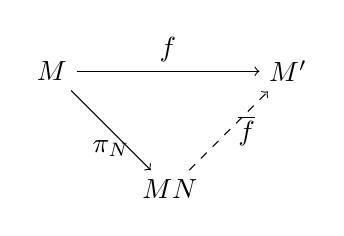
\begin{tikzpicture}
		\node (M) at (0,0) {$M$};
		\node (MS) at (3,0) {$M'$};
		\node (Q) at (1.5,-1.5) {\qraum{$M$}{$N$}};
		\draw[->, above] (M) to node {$f$} (MS);
		\draw[->, below] (M)  to node {$\pi_N$} (Q);
		\draw[->, right, dashed] (Q)  to node {$\overline{f}$} (MS);
		\end{tikzpicture}
	\end{center}
\end{proposition}
\begin{proof}
	Analog zu \propref{3_7_9}. Man zeigt, dass jedes $\overline{f}\in\Hom_K(\qraum{M}{N},M')$
	\begin{align}
		\overline{f}(x+N)=f(x)\quad (x\in M)\notag
	\end{align}
	erfüllen muss, und dass dies wiederum eine wohldefinierte Abbildung liefert.
\end{proof}

\begin{lemma}
	\proplbl{8_5_5}
	Durch $U\mapsto \pi_N(U)$ wird eine Bijektion gegeben zwischen
	\begin{itemize}
		\item den Untermoduln von $M$, die $N$ enthalten
		\item den Untermoduln von $\qraum{M}{N}$.
	\end{itemize}
\end{lemma}
\begin{proof}
	Sei $\mathcal{U}$ die Menge der Untermoduln von $M$, die $N$ enthalten, $\overline{\mathcal{U}}$ die Menge der Untermoduln von $\qraum{M}{N}$.
	\begin{itemize}
		\item $U\in\mathcal{U}\Rightarrow \pi_N(U)\in\overline{\mathcal{U}}$: klar, da $\pi_N$ ein Homomorphismus ist
		\item $\overline{U}\in\overline{\mathcal{U}}\Rightarrow \pi_N^{-1}\in\mathcal{U}$: klar, da $\pi_N$ ein Homomorphismus ist und $N=\Ker(\pi_N)=\pi_N^{-1}(\{0\})\subseteq \pi_N^{-1}(\overline{U})$
		\item $\overline{U}\in\overline{\mathcal{U}}\Rightarrow\pi_N(\pi_N^{-1}(\overline{U}))=\overline{U}$: klar, da $\pi_N$ surjektiv
		\item $U\in\mathcal{U}\Rightarrow \pi_N^{-1}(\pi_N(U))=U$:
		\begin{align}
			\pi_N^{-1}(\pi_N(U)) &= \bigcup_{x\in U} \pi_N^{-1}(\pi_N(x)) \notag \\
			&= \bigcup_{x\in U} \pi_N^{-1}(x+N) \notag \\
			&= \bigcup_{x\in U}(x+N) \notag \\
			&= U+N=U\notag
		\end{align}
	\end{itemize}
\end{proof}

\begin{remark}
	Das Ideal $I\unlhd R$ ist ein Untermodul des $R$-Moduls $R$, somit haben wir ein $R$-Modul $\qraum{R}{I}$ definiert. Man kann $\qraum{R}{I}$ mit einer Ringstruktur ausstatten.
\end{remark}

\begin{definition}[Quotientenring]
	Sei $I\unlhd R$ ein Ideal. Für $x\in R$ schreiben wir 
	\begin{align}
		x+I=\{x+a\mid a\in I\}\notag
	\end{align}
	Dann ist
	\begin{align}
		\qraum{R}{I}=\{x+I\mid x\in R\}\notag
	\end{align}
	der \begriff{Quotientenring} von $R$ modulo $I$ mit Addition und Skalarmultiplikation
	\begin{align}
		(x+I)+(x'+I) &= (x+x')+I\quad\forall x,x'\in R \notag \\
		(x+I)\cdot (x'+I) &= (x\cdot x')+I\quad\forall x,x'\in R\notag
	\end{align}
	Und wieder $\pi_I:R\to\qraum{R}{I}$ mit $x\mapsto x+I$.
\end{definition}

\begin{proposition}
	Addition und Multiplikation sind wohldefiniert und machen $\qraum{R}{I}$ zu einem kommutativen Ring mit Einselement. $\pi_I$ ist ein Ringhomomorphismus mit Kern
	\begin{align}
		\Ker(\pi_I) = I\notag
	\end{align}
\end{proposition}
\begin{proof}
	\begin{itemize}
		\item Addition wohldefiniert: \propref{8_5_2}
		\item Multiplikation wohldefiniert: Sind $x,x',y,y'\in R$ mit
		\begin{align}
			x+I &= x'+I\notag \\
			y+I &= y'+I\notag
		\end{align}
		Dann ist
		\begin{align}
			x-x' &= a\in R \quad\Rightarrow x = x'+a\notag \\
			y-y' &= b\in R \quad\Rightarrow y = y'+a\notag
		\end{align}
		Also
		\begin{align}
			xy = (x'+a)(y'+b) &= x'y'+\underbrace{ay'+x'b+ab}_{\in I}\notag \\
			%xy-x'y' = xy - (x-a)(x-b) = xb + ya - ab\in I \notag \\
			\Rightarrow xy+I &= x'y'+I\notag
		\end{align}
		\item $\qraum{R}{I}$ ist Ring: R1 bis R3 folgen aus den entsprechenden Eigenschaften von $R$.
		\item $\qraum{R}{I}$ ist kommutativ: folgt auch aus den Eigenschaften von $R$.
		\item Einselement: $1+I$
		\item $\pi_I$ ist ein Ringhomomorphismus: folgt nach Definition
		\item $\Ker(\pi_I)$: klar
	\end{itemize}
\end{proof}

\begin{proposition}[Homomorphiesatz für Ringe]
	Sei $\phi:R\to R'$ ein Ringhomomorphismus, $I\unlhd R$ ein Ideal mit $I\subseteq \Ker(\phi)$. Dann gibt es genau einen Ringhomomorphismus mit $\overline{\phi}:\qraum{R}{I}\to R'$, sodass $\overline{\phi}\circ \pi_I=\phi$.
	\begin{center}
		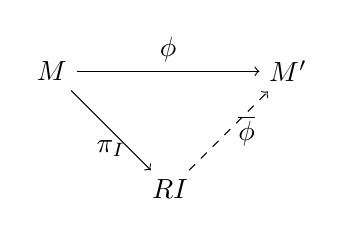
\begin{tikzpicture}
		\node (R) at (0,0) {$M$};
		\node (RS) at (3,0) {$M'$};
		\node (Q) at (1.5,-1.5) {\qraum{$R$}{$I$}};
		\draw[->, above] (R) to node {$\phi$} (RS);
		\draw[->, below] (R)  to node {$\pi_I$} (Q);
		\draw[->, right, dashed] (Q)  to node {$\overline{\phi}$} (RS);
		\end{tikzpicture}
	\end{center}
\end{proposition}
\begin{proof}
	Man sieht, dass 
	\begin{align}
		\overline{\phi}(x+I)=\phi(x)\quad\forall x\in R\notag
	\end{align}
	gelten muss, und das dies auch ein wohldefinierter Ringhomomorphismus ist.
\end{proof}

\begin{example}
	\begin{itemize}
		\item $R=\whole$, $\forall n\in\natur$ ist $n\whole$ ein Ideal.
		\begin{align}
			\qraum{\whole}{(n)}=\whole\backslash n\whole\notag
		\end{align}
		\item Sei $K$ ein Körper und sei $a\in K$. Dann ist $K[t]\to K$, $P\mapsto P(a)$ ist ein Ringepimorphismus. Der Kern $\Ker(\phi)=(t-a)$, also alle Polynome, die in $a$ eine Nullstelle haben. Es folgt
		\begin{align}
			\qraum{K[t]}{(t-a)}\cong K\notag
		\end{align}
	\end{itemize}
\end{example}

\smiley{} $\whole$ ist der Herr der Ringe \smiley{}

\begin{example}
	Sei $0\neq p\in K[t]$. $\qraum{K[t]}{(p)}$ ist ein Ring, aber auch ein $K[t]$-Modul und damit ein $K$-Vektorraum.
	\begin{align}
		\dim_K\left( \qraum{K[t]}{(p)}\right) = n= \deg(p)\notag
	\end{align}
	Ist $B=(1,\overline{t},...,\overline{t^{n-1}})$ eine Basis wobei $\overline{x}=\pi_{(p)}(x)$ $\forall x\in K[t]$.
\end{example}
\section{Der Elementarteilersatz}

Sei $R$ Hauptidealring.

\begin{definition}
	Seien $a,b,x,y\in R$. Für $i,j\in\{1,...,n\}$ ist
	\begin{align}
		E_{ij} = (\delta_{\sigma,i},...,\delta_{\mu,j})_{\sigma,\mu}\in\Mat_n(\real)\notag
	\end{align}
	Sei
	\begin{align}
		E_{ij}(a,b,x,y) = \mathbbm{1}_n-E_{ii}-E_{jj}+aE_{ii}+bE_{ij}+xE_{jj}+yE_{ji}\notag
	\end{align}
	%TODO: Matrix ergänzen von Pascal
\end{definition}

\begin{lemma}
	Ist $ax-by\in R^\times$, so ist
	\begin{align}
		E_{ij}(a,b,x,y)\in \GL_n(\real)\notag
	\end{align}
\end{lemma}
\begin{proof}
	Folgt aus LAAG1 IV.3.4, da
	%TODO: Verlinkung
	\begin{align}
		\det(E_{ij}(a,b,x,y))=ax-by\in R^\times\notag
	\end{align}
	Oder direkt: Das Inverse ist $E_{ij}(xc^{-1},bc^{-1}, ac^{-1},-yc^{-1})$, zum Beispiel
	\begin{align}
		\begin{pmatrix} a & b \\ y & x\end{pmatrix}\begin{pmatrix}xc^{-1} & -bc^{-1} \\ -yc^{-1} & ac^{-1}\end{pmatrix}=\begin{pmatrix}(ax-by)c^{-1} & 0 \\ 0 & (ax-by)c^{-1}\end{pmatrix}\notag
	\end{align}
\end{proof}

\begin{remark}
	Multiplikation von $E_{ij}(a,b,x,y)$ von links an $A$ führt eine Zeilenumformung durch: Sind $a_1,...,a_n$ die Zeilen von $A$, so wird $a_i$ durch $aa_i+ba_j$ ersetzt, und gleichzeitig $a_j$ durch $ya_i+xa_j$ ersetzt. Ist $ax-by=1$, so sind diese Zeilenumformungen invertierbar.
	
	\emph{Spezialfälle}: elementare Zeilenumformungen von Typ II und III aus Kapitel III (LAAG 1). Warnung: Im Gegensatz dazu sind über einem Ring $R$ die elementaren Zeilenumformungen vom Typ I (Multiplikation mit einem Skalar) nicht immer invertierbar!
	
	Multiplikation mit $E_{ij}(a,b,x,y)$ von rechts führt entsprechende Spaltenumformungen durch.
\end{remark}

\begin{theorem}[Elementarteilersatz für Matrizen, \person{Smith}-Normalform]
	Sei $A\in\Mat_{m\times n}(\real)$. Es gibt $0\le r \le\min\{n,m\}$, $S\in\GL_m(R)$, $T\in\GL_n(R)$
	mit 
	\begin{align}
		SAT &= \begin{pmatrix}d_1 & & & \\ & \ddots & & \\ & & d_r & \\ & & & \mathbb{0}\end{pmatrix} \notag \\
		\mathbb{0} &\in\Mat_{m-r\times n-r}\notag
	\end{align}
	wobei $d_i\in R\backslash\{0\}$ mit $d_i\mid d_{i+1}$ für $i=1,...,n-1$
\end{theorem}
\begin{proof}
	Induktion nach $\min\{m,n\}$. Für $a\in R$ sei $\delta(a)\in\natur_0\cup\{\infty\}$ die Anzahl der Primelemente in der Primfaktorzerlegung von $a$, mit $\delta(0):=\infty$, und $\delta(A):=\min_{ij}\{\delta(a_{ij})\}$. Wir können annehmen, dass $\delta(A)\le \delta(SAT)$ für alle $S\in \GL_m(R)$ und $T\in \GL_n(R)$. Durch Zeilen- und Spaltenvertauschungen erreichen wir, dass $\delta(a_{11})=\delta(A)$.
	\begin{itemize}
		\item \emph{1. Behauptung:} $a_{11}\mid a_{i1}$ für alle $i$. Gäbe es ein $i\ge 1$ für dass $a_{11}\nmid a_{i1}$, so sei $c=\ggT(a_{11},a_{i1})=xa_{11}+ya_{i1}$ mit $\ggT(x,y)=1$, also $ax-by=1$ mit $a,b\in R$. Multiplikation mit $E_{1i}(x,y,a,b)$ von links erzeugt an der Position $(1,1)$ das Element $c$, und $\delta(c)<\delta(a_{11})=\delta(A)$, im Widerspruch zur Minimalität von $\delta(A)$. \\
		Analog zeigt man, dass $a_{11}\mid a_{1j}$ für alle $j$. Durch Zeilen- und Spaltenumformungen können wir deshalb nun $a_{i1}=0$ für alle $i>1$ und $a_{1j}$ für alle $j>1$ erreichen.
		\item\emph{2. Behauptung:} $a_{11}\mid a_{ij}$ für alle $i,j$. Gäbe es $i>1$ und $j>1$ mit $a_{11}\nmid a_{ij}:=b$, so können wir die $j$-te Spalte zur ersten Spalte addieren, was $a_{11}$ nicht ändert und $a_{1i}=b$ bewirkt. Wider können wir Behauptung 1 anwenden und erhalten den Widerspruch, dass $a_{11}\mid b$. Damit ist nach diesem Umformungen
		\begin{align}
			A=\begin{pmatrix}a_{11} & \\ & a_{11}\cdot A'\end{pmatrix}\notag
		\end{align}
		mit $A'\in\Mat_{(m-1)\times (n-1)}(R)$. Wir wenden nun die Induktionshypothese auf $A'$ an und sind fertig.
	\end{itemize}
\end{proof}

\begin{remark}
	Man kann zeigen, dass die $d_1,...,d_r$ bis auf Assoziiertheit eindeutig bestimmt sind. Man nennt sie deshalb \begriff{Elementarteiler} der Matrix $A$.
\end{remark}

\begin{example}
	Sei $R=\whole$. Bestimme die Elementarteiler der Matrizen
	\begin{align}
		\begin{pmatrix}0&1\\1&0\end{pmatrix},\begin{pmatrix}1&2 \\ 3&4\end{pmatrix},\begin{pmatrix}2&0&0 \\ 0&4&0 \\0&0&6\end{pmatrix}\notag
	\end{align}
\end{example}

\begin{mathematica}[\person{Smith}-Normalform]
	Elementarteiler lassen sich mit Mathematica mit der Funktion
	\begin{align}
		\text{\texttt{SmithDecomposition[]}}\notag
	\end{align}
	die als einziges Argument eine Matrix braucht. Allerdings ist der Output unformatiert, mit folgenden Befehl sieht das deutlich besser aus:
	\begin{align}
	\text{\texttt{MatrixForm/@ (\{u,r,v\} = SmithDecomposition[])}}\notag
	\end{align}
	Der Output sind 3 Matrizen, wobei \texttt{u} für $S$, \texttt{v} für $T$ und \texttt{r} für das Ergebnis von $SAT$ steht.
\end{mathematica}

\section{Zyklische Vektorräume}

Sei $K$ ein Körper, $V$ ein $n$-dimensionaler $K$-Vektorraum, $f\in\End_K(V)$.

\begin{conclusion}[\person{Frobenius}-Normalform]
	Es gibt eine Basis $B$ von $V$, für die 
	\begin{align}
		M_B(f)=\diag(M_{P_1},...,M_{P_m})\notag
	\end{align}
	mit $P_1,...,P_m\in K[t]$ normiert, die $P_i\mid P_{i+1}$ erfüllen.
\end{conclusion}

\part*{Anhang}
\addcontentsline{toc}{part}{Anhang}
\appendix

\chapter{Listen}
\section{Liste der Theoreme}
\theoremlisttype{allname}
\listtheorems{theorem}

\pagebreak
\section{Liste der benannten Sätze, Lemmata und Folgerungen}
\theoremlisttype{optname}
\listtheorems{proposition,lemma,conclusion}

\pagebreak
\section{Liste der Mathematica/WolframAlpha-Befehle}
\smiley{} für faule Mathematiker \smiley{} \\
\theoremlisttype{allname}
\listtheorems{mathematica}

%\printglossary[type=\acronymtype]

\printindex

\end{document}